% Use the University of Michigan thesis class.
\documentclass[thesis,openany]{./tex/thesis-umich}

\newcommand*{\ATLASLATEXPATH}{latex/}
\usepackage{\ATLASLATEXPATH atlasphysics}
\usepackage{ANA-HIGG-2020-16-INT1-defs}

\usepackage{pgffor}
\usepackage{longfigure}
\usepackage{mathtools}
\usepackage{bm}
\usepackage{multirow}
\usepackage[export]{adjustbox}
\usepackage{mathrsfs}
\usepackage{float}
\usepackage{makecell}
\usepackage{lscape}
\usepackage{pdflscape}
\usepackage{amsmath}

\usepackage{rotating}
\usepackage{etoolbox}
\usepackage{tikz}

\usepackage{siunitx}
% High energy physics
\DeclareSIUnit\micron{\micro\metre}
\DeclareSIUnit\mrad{\milli\rad}
\DeclareSIUnit\gauss{G}
\DeclareSIUnit\eVperc{\eV\per\clight}
\DeclareSIUnit\nanobarn{\nano\barn}
\DeclareSIUnit\picobarn{\pico\barn}
\DeclareSIUnit\femtobarn{\femto\barn}
\DeclareSIUnit\attobarn{\atto\barn}
\DeclareSIUnit\zeptobarn{\zepto\barn}
\DeclareSIUnit\yoctobarn{\yocto\barn}
\DeclareSIUnit\nb{\nano\barn}
\DeclareSIUnit\pb{\pico\barn}
\DeclareSIUnit\fb{\femto\barn}
\DeclareSIUnit\ab{\atto\barn}
\DeclareSIUnit\zb{\zepto\barn}
\DeclareSIUnit\yb{\yocto\barn}




% Title of the thesis
\title{My Thesis}

% Author name
\author{Name}

% Department
\department{Department}

% Year of completion
\year=2020

% ORCID ID 
\orcid{My Orcid ID}

% UM Unique Name 
\umuniquename{name}

% Frontispiece
%\frontispiece{\includegraphics[width=4in]{./pics/frontispiece.pdf}}

% Default style for front pages
\frontpagestyle{1}

% Dedication
\dedication{ “Questing Physicks isn’t like the Quiet and Queer branches. You can’t do it at home in a comfortable chair—you have to be out in the thick of the business, with your tools on your belt and your heart on your sleeve!” - Catherynne Valente, The Girl Who Fell Beneath Fairyland and Led The Revels There \ref{cite:Fairyland}. \\


For }


% Acknowledgments
\acknowledgments[6]{
% The acknowledgements section of this dissertation, perhaps surprisingly, is the hardest for me to write. If left to my own devices, I have no doubt that the list of people I'd want to thank would be as long as the rest of this paper, if not longer. Like the globe held up by the Atlas of myth, my world is perched upon the shoulders of giants. Completing a dissertation at any point is no easy task, let alone in the middle of a pandemic- I could not have done this alone.

%First, to my family- to my parents, Gregg and Gretchen, thank you for working so hard to foster a lifelong sense of curiosity in me, in a world that doesn't always value it. Without the endless stream of NOVA specials, public lectures, and museum trips, I would not be the person I am today.

%To my brother Grant, thank you for 

%To my grandparents, JoAnn and Ray, Ray and Sue, and Bert and Ron- thank you for

%Most of all, of course, thanks to my partner, Abigail Goodhart, who

}
% This command sets the width of the acknowledgments area as a fraction
% of the total width of the text area.
%\acknowledgmentswidth{0.85}

% Preface
%\preface[2]{ Do I need this?}

% Committee
\committee{ %
Thomas Schwarz, Chair \\
Dante Amidei \\ 
Junjie Zhu \\ 
James Liu \\ 
Eric Bell \\ }

% Chair must be entered separately for formatting reasons.
\chair{Thomas Schwarz}

% Commands to hide or show lists of figures, tables, etc.
%\hidelistoftables
%\showlistofprograms
\showlistofappendices

% Definition of any abbreviations used.
\abbreviations{ %
    \acro{TH}{Thesis}
    \acrodefplural{TH}{Theses}   
}



% Some abstract text
\abstract{ %
My Abstract. 
}
%\hideabstractpagenumber

%% DOCUMENT AREA
\usepackage{ amssymb }
\usepackage{ amsmath }
\begin{document}

% ----- Introduction ----- %

\chapter{An Overview of the Standard Model} \label{chap:theory_chapter}
	\usepackage{ amssymb }

\section{The Standard Model} \label{sec:SM} 

The Standard Model of Particle Physics is arguably one of the crowning achievements of the last century of physics research. Though it is doubtless incomplete (it does not, for instance, explain the dark energy or dark matter observed in cosmological experiments, nor does it provide a satisfactory quantum-mechanical model of gravity), all predictions it has made have yet to be falsified \ref{Peskin}, \ref{Gordy}, \ref{FTGA}, \ref{Griffiths}.

The Standard Model is a quantum field theory, meaning that it describes the behavior of fields (physical quantities that are defined at all points in spacetime; common examples of fields include electric and magnetic fields) and their discrete, quantized excitations, referred to as particles (common examples of particles are the electron and the photon, which are excitations of the "electron field" and the electromagnetic field respectively). More about the mathematics of field dynamics will be discussed in section \ref{sec:Lagrangians}.

The Standard Model divides these fundamental particles (and their corresponding fields) into two major categories: the bosons and the fermions. Fermions carry half-integer spin, while bosons carry integer spin. In a general sense, the elementary fermions can be thought of as the particles that comprise matter, while the elementary bosons can be thought of as the particles that correspond to the behavior of the four fundamental forces (electromagnetism, the strong nuclear force, the weak nuclear force, and gravity).

The elementary fermions of the Standard Model all have spin $1/2$. They are divided into two major subgroupings, quarks and leptons; each of these is further divided into three generations. Each generation of quarks contains one up-type quark (up, charm, or top) and one down-type quark (down, strange, and bottom), while each generation of leptons contains one charged lepton (electron, muon, or tau) and one neutrino (electron neutrino, muon neutrino, or tau neutrino). Fermions of successive generations behave similarly to each other, though those of each subsequent generation are more massive than the last.

The quarks are the only fermions that undergo both the strong and weak nuclear interactions, and are also the only particles in the Standard Model that have fractional electromagnetic charge ($+2/3$ for up-type quarks and $-1/3$ for down-type quarks). However, because quarks are never found in isolation and are always bound to other quarks in composite states called hadrons, all observable quark final states have integer charge. Conversely, the charged leptons all have an electromagnetic charge of $-1$, while neutrinos are chargeless. While the quarks and charged leptons have precisely-measured masses, the mass of the neutrinos is vanishingly small, and, to date, only the differences between the different neutrino masses have been conclusively measured.

In addition to these 12 fermion species, each fermion species has a corresponding antimatter "antifermion" species, which has the opposite charge and parity quantum numbers. This is discussed at length in section \ref{sec:CPT}.

The bosons of the standard model are the "messengers" through which the fundamental forces operate (with the exception of the Higgs boson, which is detailed at length in section \ref{sec:EWSB}). The photon and the gluons are massless, while the two W-bosons, the Z-boson, and the Higgs boson are all massive. The photon is the mediator of the electromagnetic force and couples to charged particles; the gluon is the mediator of the strong nuclear force and couples to particles with "color charge", and the W and Z bosons are the mediators of the weak nuclear interaction, coupling to all fermions with left-handed parity and antifermions with right-handed parity. In addition, the three weak bosons ($W^{+}$, $W^{-}$, and $Z$) can all couple to each other, as can the gluons.

The strong nuclear interaction binds quarks together, while the weak interaction governs the decay of one species of fermion into another. Weak interactions operate primarily on fermion doublets, coupling each up-type quark to its corresponding down-type quark and each charged lepton to its corresponding neutrino. However, some intergenerational coupling does occur, the rarity of which is governed by a matrix of coefficients called the Cabibbo-Kobayashi-Makasawa (or CKM) matrix. 

The Higgs boson is the only scalar (spin-0) boson in the Standard Model. Though it does not mediate any force directly, its existence is a consequence of the unification of the electromagnetic and weak nuclear interactions into one "electroweak" interaction at high energy scales. Without the role of the Higgs boson in this process, the fermions, the W-bosons, and the Z-boson would all be massless; thus, the Higgs can be said to "give mass" to the particles of the Standard Model. It couples to all massive particles in the Standard Model, namely, the fermions and the W and Z bosons.

\subsection{sec:Lagrangians, Fields, and Gaug}

In order to fully explain the Higgs mechanism, we must first discuss the mathematical language of quantum field theory. Both quantum and classical field theories are often discussed using Lagrangian dynamics, where the Lagrangian is defined as  $\mathcal{L} = T - V$, the difference of the kinetic and the potential energy. Physical properties will always evolve in such a way that the integral of this property with respect to time, $\mathcal{S} = \int \mathcal{L} dt$, called the action, is a constant. Lagrangians are also incredibly useful in that they give rise to conservation laws: Noether's Theorem states that operations performed on a system that do not change the Lagrangian are each associated to conserved quantities of a system (i.e., systems with translationally invariant Lagrangians must respect conservation of momentum, systems with temporally-invariant Lagrangians must respect conservation of energy, etc.).

A variety of types of fields exist, but we will discuss three at length: Klein-Gordon fields, which are scalar fields (single quantities defined everywhere), Dirac spinor fields (vector quantities defined everywhere), and gauge fields (additional vector fields that must be introduced in order to preserve certain physical symmetries. We begin with the Klein-Gordon field.

Klein-Gordon fields, one of the simplest examples of a field, are real scalar-valued quantities often denoted using the symbol $\phi$. A non-interacting "free" Klein-Gordon field evolves according to the Lagrangian:

\begin{equation}
\mathcal{L} = T - V 
=\frac{1}{2} \frac{\partial^{2} \phi}{\partial t^{2}} - \frac{1}{2} (\nabla \phi)^{2} - \frac{1}{2} m^{2} \phi^{2}
=-\frac{1}{2}(\partial^{\mu}\phi)(\partial_{\mu}\phi)- \frac{1}{2} m^{2} \phi^{2}
\end{equation}

where we utilize Einstein sum notation in the last line to compress the four derivatives in the preceding expression into a single shorthand symbol. The Lagrangian of an interacting Klein-Gordon field would look similar, but would possess additional $V$ potential terms depending on the nature of the interaction. As the only scalar in the Standard Model, the observable Higgs boson is the only elementary particle to follow an interacting Klein-Gordon field equation.

While the concept of a complex-valued scalar field does not directly correspond to any of the physical elementary particles that are present in the Standard Model, it plays an important role in the understanding of the Higgs mechanism. A complex-valued scalar field behaves similarly to a real-valued one, with the Lagrangian

\begin{equation}
\mathcal{L} = (\partial^{\mu}\phi^{*})(\partial_{\mu}\phi) - \frac{1}{2} m^{2} \phi^{*} \phi
\end{equation}

Where * denotes the complex conjugate of the scalar field.

Finally, Dirac fields describe all Standard Model fermions (with the possible exception of neutrinos). They are vector fields as opposed to scalar fields, and behave according to the Lagrangian:

\begin{equation}
\mathcal{L} = \bar{\psi}(i \gamma^{mu} \partial_{mu} - m) \psi
\end{equation}

where $\gamma^{mu}$ denotes the set of Dirac gamma matrices, and $\bar{\psi} = \psi^{\dagger} \gamma^0$ denotes the transpose of the complex conjugate of the vector field multiplied by one of these matrices, defined as such in order to preserve invariance under relativistic Lorentz boosts. 

A four-component Dirac vector field can be written in a variety of representations, but one of the most useful is that of a doublet of two two-component Weyl spinors, one left-handed and one right-handed, that is, $\psi = \begin{pmatrix} \psi_L \\ \psi_R \end{pmatrix}$. Each of these components transforms differently under Lorentz boosts.

In order to discuss the gauge fields corresponding to the Standard Model bosons, we must first discuss the concept of gauge symmetries. Consider a single Dirac vector field described by equation \ref{eq:Dirac}. We transform the field by rotating it by a constant phase $\alpha$:  $\psi \rightarrow e^{i \alpha} \psi $, $\bar{\psi} \rightarrow e^{-i \alpha} \bar{\psi} $.

\begin{equation}
\mathcal{L} = - (e^{-i \alpha} \bar{\psi})(i \gamma^{mu} \partial_{mu} - m) (e^{i \alpha} \psi)
= - (e^{-i \alpha} e^{i \alpha})\bar{\psi} (i \gamma^{mu} \partial_{mu} - m)\psi
= -\bar{\psi}(i \gamma^{mu} \partial_{mu} - m) \psi
\end{equation}

We see that we recover the original Dirac Lagrangian. Thus, the lagrangian is invariant under a constant phase rotation. A transformation of this charater is called a global gauge transformation. A one-dimensional rotation is a unitary transformation, so we call this a global $U(1)$ gauge symmetry.

We next consider the concept of a local gauge transformation, that is, one in which the phase $\alpha$ may vary with position. The field transforms, as before, like  $\psi \rightarrow e^{i \alpha (x)} \psi $, $\bar{\psi} \rightarrow e^{-i \alpha (x)} \bar{\psi} $. However, we note that the dependence on position means that we can no longer factor out the exponentials, and we thus have

\begin{equation}
\mathcal{L} = - (e^{-i \alpha (x)} \bar{\psi})(i \gamma^{mu} \partial_{mu} - m) (e^{i \alpha (x)} \psi)
=-i e^{-i \alpha (x)} \bar{\psi} \gamma^{mu} (e^{i \alpha (x)} \partial_{mu} \psi + i e^{i \alpha (x)} \psi \partial_{mu} \alpha -m \bar{psi}\psi
=-\bar{\psi}(i \gamma^{mu} \partial_{mu} + \gamma^{mu} \partial_{mu} \alpha - m) \psi
\end{equation}

i.e., the Lagrangian is not invariant under this sort of transformation. However, local gauge invariance is an important physical symmetry, so in order to attempt to preserve it, we add an additional term to the original Lagrangian: an extra vector field $A_\mu$ that transforms like $A_\mu \rightarrow A_\mu - \frac{1}{q} \partial_{mu} \alpha(x) $ for a constant q. We also define a new operator, called the covariant derivative: $D_{mu} = \partial_{mu}+ iqA_{mu} $. Given how $A_{mu}$ transforms, we see that $D_{mu}$ transforms like

\begin{equation}
D_{mu} = \partial_mu + iqA_{mu}
\rightarrow \partial_mu + iq(A_{mu}-frac{1}{q}\partial_{mu}\alpha(x))
= \partial_mu + iqA_{mu}-i\partial_{mu}\alpha(x)
=D_{mu}-i\partial_{mu}\alpha(x)
\end{equation}

Let us replace the $\partial_{mu}\phi$ terms in the initial Lagrangian with $\D_{mu}\phi$ and transform.

\begin{equation}
\mathcal{L} = - (e^{-i \alpha (x)} \bar{\psi})(i \gamma^{mu} (D_{mu}-i\partial_{mu}\alpha(x)) - m) (e^{i \alpha (x)} \psi)
=-(e^{-i \alpha (x)} \bar{\psi})(i \gamma^{mu} (\partial_mu + iqA_{mu}-i\partial_{mu}\alpha(x))-m)(e^{i \alpha (x)} \psi)
=-\bar{\psi}(i \gamma^{mu} \D_{mu} + \gamma^{mu} \partial_{mu} \alpha - \gamma^{mu} \partial_{mu} \alpha - m) \psi
=-\bar{\psi}(i \gamma^{mu} \D_{mu} - m) \psi
\end{equation}

Thus, by introducing an additional vector field that corresponds to the local U(1) gauge symmetry, we have restored the invariance of our lagrangian. Physically, this field is analogous to the introduction of electromagnetism to our single Dirac fermion model, with the $A_mu$ field playing the role of the photon: it is a vector quantity and so has spin-1, it must be massless (as adding an $A_mu$ mass term to the Lagrangian would violate the symmetry again), and couples to the fermion fields according to their electromagnetic charge. We note that we can also still preserve invariance if we add an additional term $L_{kin} = -\frac{1}{4}F^{\mu \nu} F_{\mu \nu}$ to the Lagrangian, where $F_{\mu \nu} = \partial_{\mu} A_{\nu} - \partial_{\nu} A_{\mu}$: this corresponds to the energy inherent in electromagnetic fields themselves. 

Each of the fundamental forces in the Standard Model can be understood in terms of these sorts of gauge symmetries. The photon is the particle excitiation of the electromagnetic field, which corresponds to a one-dimensional rotation "U(1)" transformation. In order to be invariant under three dimensional transformations of the type "SU(3)" (the set of all volume-preserving, $\bar{\psi}\psi$-preserving transformations in a 3D vector space), we must add eight new vector fields (these are the eight gluons), leading to the incorporation of the strong interaction into the Standard Model.

Similarly, in order to be invariant under two-dimensional transformations of the type "SU(2)" (the set of all volume-preserving, $\bar{\psi}\psi$-preserving transformations in a 2D vector space), we must add three new vector fields. However, these cannot be the observed weak-interaction bosons, the $W^{+}, W^{-} and Z$: as mentioned before, the new fields must be massless, as adding a mass term for these bosons would violate the local gauge symmetry. How, then, can the masses of the weak bosons fit into the Standard Model? The answer lies in the introduction of yet another field, called the Higgs field, the particle excitation of which is the much-lauded Higgs boson.

\section{The Higgs Mechanism and Electroweak Symmetry Breaking} \label{sec:EWSB} 

By now, it should be clear that the Higgs field is important not simply because it "gives particles mass" (an often-made claim which is, in a sense, true), but because it is a vital missing piece of the Standard Model that is necessary to reconcile the elegant mathematical language of the fundamental interactions with the particles we observe in real-world experiments.

To understand the Higgs mechanism, we must first devote a brief detour to the concept of symmetry breaking. This occurs when an unstable, symmetric state spontaneously changes into a more stable, symmetric one. Consider, for example, the "wine-bottle" potential shape depicted in figure \ref{fig:potential}.

\begin{figure}
\end{figure}

When the ball is balanced at the top of the potential "hill", the configuration is spatially symmetric: that is, no direction is privileged over any other. However, when this delicate balance is even slightly disturbed, the ball will roll down the hill in some direction, resulting in a final state that is \emph{not} symmetrical. This is the phenomenon known as "spontaneous symmetry breaking".

Using the language of quantum field theory, we can easily add spontaneously-breakable symmetric potential terms to a Lagrangian. If we do so, the phenomenon of symmetry breaking allows us to rewrite these terms as a combination of massless fields (one for each "choice" the symmetry breaking must make) and massive fields (corresponding to the leftover degrees of freedom). If we rewrite the "wine-bottle" potential in this way, for example, the one new massless field corresponds to the ball's angular position along the circle at the base, while the massive field corresponds to the ball's  radial position "up" or "down" the hill. The massless particles that arise from these massless fields are known as Goldstone bosons.

We are now ready to discuss the Higgs mechanism. We write the terms of the Standard Model Lagrangian, noting that, since the weak interaction is observed to be chiral, it may couple differently to left- and right-handed fermions.

We can combine the electromagnetic and weak nuclear forces as different manifestations of the same force, called the electroweak force, that transforms like $U(1) \cross SU(2)$.

In this case, the generator of the U(1) symmetry ($frac{\alpha}(x)$) is not the electric charge $Q$ as in our previous example, but is instead the "Weak Hypercharge" $Y = 2(Q -I_{3})$, where $I_{3}$ is the "Weak Isospin". For right-handed particles, $I_{3} = 0$, for left-handed up/charm/top quarks and neutrinos, $I_{3} = +frac{1}{2}$, and for left-handed down/strange/bottom quarks and charged leptons, $I_{3} = +frac{1}{2}$.






\section{The Higgs Boson and Its Couplings} \label{sec:example_subsubsection} 

This is a subsubsection. It will not be included in the table of contents. 

\section{CP-Symmetry}
We return to the Dirac field to discuss its properties. 
 

\chapter{The ATLAS Detector} \label{chap:detector_chapter}
	\section{The Large Hadron Collider} \label{sec:LHC} 

At roughly 27 kilometers in circumference, the Large Hadron Collider (LHC) at the Center for European Nuclear Research (CERN) is the largest machine ever built, slicing through the solid rock of the Jura mountains and running more than 100 meters beneath the Swiss-French border \ref{LHC}. It is a proton-proton collider operating at a center-of-mass energy of 13 TeV, circulating two beams of protons in opposite directions, each at more than 99\% the speed of light \ref:{speed}. By utilizing a system of radiofrequency (RF) cavities and dipole magnets, protons are delivered to four primary collision points in bunches spaced 25 nanoseconds apart \ref:{40Mhz}.

The LHC achieves such a powerful center-of-mass energy by repurposing a significant fraction of older collider physics infrastructure, including the Super Proton Synchrotron (SPS), which was itself one of the most powerful particle accelerators in the world at one time. In order to achieve collision, hydrogen atoms are first stripped of their electrons using an ionizing cathode filament in a device called a 'Duoplasmatron'; this produces a plasma that is filtered to produce beams of protons \ref{}. The LINAC2, a linear accelerator, then accelerates the resultant proton beams to a collision energy of 50 MeV; the beams then move to the Proton Synchrotron Booster (PSB), a circular accelerator that accelerates them to an energy of 1.4 GeV, followed by the Proton Synchrotron (PS), a second circular accelerator that accelerates them to 25 GeV. Following this, beams enter the aforementioned Super Proton Synchrotron, where they are accelerated to a collision energy of 450 GeV before being injected into the Large Hadron Collider ring. This infrastructure is depicted in Figure \ref{fig:LHC}.

The tight bunching of protons by the LHC ring allows the collider to deliver collisions at a high luminosity, a measure of the number of expected collision events per unit of beam area. Luminosity is measured in both instantaneous and integrated form (i.e., 'luminosity per unit time' and total luminosity delivered to date'); as of the end of the second major LHC run, the collider has delivered a total integrated luminosity of XXX fb^{-1}, equivalent to X.XX*10^{41} collisions per square centimeter \ref{lumi}. 

At the time of this writing, the LHC is nearing the end of 'Long Shutdown 2' (LS2), a two-year long upgrade period designed to increase detector performance and lay the groundwork for the upcoming high-luminosity LHC (HL-LHC) upgrade, which is slated to begin in approximately 2027 and aims to increase the design luminosity of the LHC by at least a factor of 5 \ref:{HL-LHC}. Higher luminosity allows for the production of more rare physics events, but also dramatically increases the incidence of unwanted "pileup" events; mitigating this is one of the major efforts of the CERN physics community during the lead-up to the HL-LHC run.

The LHC ring accelerates beams to a center-of-mass collision energy of 13 TeV. The ring consists of two primary beam pipes, one containing a "clockwise" beam and the other containing a "counterclockwise" beam, which overlap at the four primary collision points. These correspond to the four major LHC physics experiments: ATLAS  \ref{} and CMS \ref{}, which are "general purpose" physics detectors, LHCb \ref{}, which is specialized to study the physics of hadrons containing bottom (or "beauty") quarks, and ALICE \ref{}, which is primarily designed for heavy-ion physics. Due to the highly sensitive nature of their instrumentation, these detectors are buried approximately 100 meters underground to avoid interference from high-energy cosmic rays.

\section{The ATLAS Detector} \label{sec:ATLAS} 

The work contained in this dissertation was performed using the ATLAS (A Large Toroidal LHC ApparatuS) detector. Together with its "sibling detector" CMS (the Compact Muon Solenoid), the ATLAS detector is one of CERN's two "general purpose" detectors, so-called because it is designed to observe a wide variety of high-energy physics phenomena. The ATLAS detector is cylindrical, with a diameter of 25 meters and a length of 44 meters \ref{ATLAS}. Upon colliding at the interaction point in the center of the detector, each proton's constituent particles will interact with one another through a host of different physical processes, producing a variety of new particles traveling at high velocities. The ATLAS detector is comprised of several specialized subsystems, each of which is responsible for logging different properties of these decay products. Each of these subsystems is optimized to detect specific particles and properties; taken together, they provide a detailed picture of a collision event much like different color channels in a photographic camera.
	The Inner Detector (ID), a high-resolution detector composed of silicon "strips", "pixels", and "straws", measures the tracks of particles close to the primary vertex. It is encased within a 2T solenoidal magnetic field that bends the tracks of charged particles produced at the collision point, allowing their momenta to be measured as a function of the curvature of their trajectories. Enclosing the Inner Detector are two nested calorimeters: one scintillator-tile electronic calorimeter (ECAL) that measures the energy of incident photons and electrons, and one liquid-argon hadronic calorimeter (HCAL) that measures the energy of hadronic showers. Finally, a muon spectrometer composed of gas-filled tubes and chambers records the tracks of muons, which do not decay in the calorimeters like most other particles due to their status as minimum-ionizing particles \ref{muons}. The muon spectrometer has three major subsystems, a cylindrical barrel and two circular endcaps, which provide spatial coverage in both the central and forward regions of the ATLAS detector. The entirety of the muon spectrometer is suffused with magnetic field generated by 24 toroidal magnets, eight of which lie in the barrel and generating a field of 1T and eight of which lie in each endcap generating a field of 0.5T. These magnets bend the trajectories of muons in a manner similar to the inner solenoidal magnet system, allowing the momenta of particles to be measured based on the track curvature. The ATLAS detector is also equipped with a highly sensitive trigger system, which uses a wide variety of physics signatures in each of these detector subsystems to determine which collision events to store for later analysis \ref{ATLAS}.
	The ATLAS detector uses a right-handed coordinate system, with the central interaction point at z = 0. The x-axis points from the interaction point to the center of the LHC ring, while the y-axis points upward. However, particle trajectories are more commonly measured not in (x,y,z) coordinate space but utilizing angular variables (\(r\) and \( \phi \)) in the transverse plane and pseudorapidity \( \eta \) in the longitudinal plane, where \( \eta = -ln(tan( \theta /2) ) \). This is illustrated in figure \ref{fig:coords}.

\subsection{Inner Detector} \label{sec:ID} 

The Inner Detector is composed of five highly granular subdetectors. The closest to the beam, the silicon-based Insertable B-Layer, was added between the LHC's first and second runs in order to improve precision track-vertex measurement for tasks such as b-hadron tagging and \( \tau\) lepton identification \ref{IBL}, methods discussed more in section \ref{tagging}. Proceeding outward from the IBL are the silicon-based Pixel detector and Semiconductor Tracker (SCT), followed by the gas-based Transition Radiation Tracker (TRT) \ref{ATLAS}. 

The IBL is composed of 26,880 250×50 \(μm^2\) silicon pixels arranged in an 80 column by 336 row geometry. The pixel modules are supported by 14 support staves, tilted at approximately 14 degrees from the nominal to achieve near-complete cylindrical coverage of the barrel region. The IBL is approximately 33.25 mm from the beam axis, necessitating a replacement of the beryllium beam-pipe with a smaller-radius one for detector reintegration \ref{IBL}.

Silicon is an optimal material for precision trackers due to its status as a semiconductor. Silicon wafers can be easily "doped" with atoms of other elements, leading them to carry either an excess of electrons (n-type semiconductors) or a deficit of electrons (p-type semiconductors). By putting the two together, an n-p junction is formed, leading to a one-way current gate known as a diode. A voltage is then applied to the diode to halt current flow ("reverse biasing"). When ionizing particles such as those produced in collisions pass through the silicon, they will produce a cascade of charge carriers that will induce a current in the diode, which can then be measured by the precision front-end electronics attached to the silicon wafers \ref{Knoll Radiation Detection}.

The pixel detector is similarly composed of silicon pixels, each of which is either 50x400 \(μm^2\) (nominal) or 50x600 \(μm^2\) (near the front-end readout electronics due to spatial constraints). The detector contains 1744 identical pixel sensors, each of which contains 47232 pixels. Three layers of pixels in the barrel region sit at r = 50.5,  88.5 and 122.5 mm from the beam axis, while three layers of pixels in the endcap region sit at r= 495, 580, and 650 mm from the beam axis. The silicon wafers in the pixel detector are "n+ type" strips (n-type semiconductors with extra doping) embedded in an n-type bulk, rather than the traditional n-type and p-type semiconductors due to the fact that excessive radiation from the beam can cause standard n-and-p-type semiconductors to change into one another. 

The SCT is composed of longer silicon microstrip wafers made out of standard n-p type semiconductors. It consists of four layers of 2112 total silicon microstrip modules in the barrel region and 1976 microstrip modules in the endcap regions, with 770 microstrips per sensor module. The strips are 12cm long and 80 μm wide; the distance of modules from the beam pipe ranges from radii of r= 299 mm to r= 514 mm in the barrel and r=852.8 mm to r= 2720.2 mm in the endcaps. The SCT is designed using less-costly materials than the TRT and IBL, but serves a valuable complementary function.

Finally, the TRT consists of polyimide "straws" filled with a gas mixture (70\% Xenon, 27\% Carbon Dioxide, and 3\% Carbon Tetrafluoride), each 4mm in diameter and 144 cm long. In the center of each straw tube is a 31 μm in diameter grounded gold-plated tungsten wire filament that serves as an anode. Charged particles travelling through the gas medium will ionize it, producing a cascade of ions that will drift to the anode wire. The TRT is uniquely designed to detect low-energy X-ray transition radiation photons, which allows for better identification of electron candidates \ref{TRT}. The barrel region consists of 73 layers of sensor modules ranging from r= 554 mm to r = 1082 mm from the beam pipe, while the encaps straws, arranged in a "wheel" shape, stretch from r= 852.8 mm to r= 2720.2 mm from the beam pipe.

Together, these subsystems form the ATLAS detector's Inner Detector. Each subdetector has a different spatial resolution- the IBL has a resolution of XXXX, the pixel detector has a resolution of XXXX, the SCT has a resolution of XXXX, and the TRT has a resolution of XXXX. The combined effect of these subdetectors is thus to record particle tracks produced in collisions with very high granularity, allowing for sophisticated physics analyses to be performed. 

\subsection{Calorimeters} \label{sec:Calos} 

This is a subsection. It will be included in the table of contents. 


\subsubsection{ECAL} \label{sec:ECAL} 

\subsubsection{HCAL} \label{sec:HCAL} 




\subsection{Muon Spectrometer} \label{sec:Musyst}
 






\subsection{Magnets} \label{sec:Magnets}


\subsubsection{solenoid} \label{sec:solenoid} 

\subsubsection{toroid} \label{sec:toroid} 




\subsection{Trigger} \label{sec:Trigger}
Due to the high rate of collision events delivered by the accelerator 

Additionally, two Minimum Bias Trigger Scintillators, composed of plastic scintillator tiles, sit on the circular endcaps of the ID in order to provide trigger capabilities in the forward region \(|\eta| > 2.5 \). The MBTS endcap scintillator consists of 2 cm thick polystyrene scintillator disks mounted on each endcap at a distance of 3.6m from the collision point at. 
 

\chapter{Experimental Methods} \label{chap:methods_chapter}
	\section{Experimental Methods} \label{sec:methods} 

\subsection{Monte Carlo Simulation} \label{sec:MC} 
In order to accurately reconstruct and measure objects that are produced in high-energy physics collisions, a variety of high-level techniques are employed. One of the most widely-used is Monte Carlo simulation, a way of modelling expected real-world observations given certain theoretical predictions. 


Hard scatter


\subsection{Reconstruction and Tagging} \label{sec:Reco} 

Objects 

\subsection{Tracks} \label{sec:Tracks} 

Track reconstruction is essential for identifying and measuring the properties of a wide variety of physics objects, including both muons and hadronic jets.

Initially, the "space points" (spatial coordinates) of potential particle hits are reconstructed using clusters of energy deposits in both the Pixel and SCT detectors. Track candidates are then identified combinatorially using this space-point information (with a minimum of three space-points per track candidate); these track candidates are then passed through an analytic weight-based "ambiguity solver" designed to weed out unphysical track candidates. To aid the ambiguity solver, a neural network is implemented in order to distinguish between isolated and merged clusters of energy deposits. After this, a neural network-based procedure is used to fit the identified tracks. \ref{cite:tracker}.

Fitted tracks from the Pixel detector and SCT can be extended into the TRT if nearby TRT hits are identified. In addition, tracks that are seeded by TRT hits can also be identified and reconstructed using an "outside-in" approach; this helps mitigate the potential loss of real tracks at the ambiguity-solver stage \ref{cite:NEWT}.

After tracks are identified and reconstructed, they are used to identify interaction vertices in the event. Each vertex candidate must contain at least two tracks, each with transverse momentum $p_{T} > 400$ MeV and $|\eta|<2.5$, at least nine hits in the Pixel or SCT detector for tracks with $|\eta|<1.65$ or at least eleven hits for tracks with $|\eta|>1.65$, at least one hit in the first two pixel layers (i.e., the IBL and the inner b-layer), no more than one shared module (i.e. one shared pixel hit or two shared SCT hits), no holes in the Pixel detector, and no more than one hole in the SCT. An iterative combinatorial procedure is then used to fit all compatible tracks to vertex candidates; the primary vertex (PV) representing the initial protom-proton collision is chosen as the vertex with the greatest $\Sigma p_{T}^{2}$ \ref{cite:VertexMeloni}.

However, we note that, for $H \rightarrow \gamma \gamma$ events, a potential lack of charged particles in the final state means that a different primary-vertexing method utilizing ECAL clusters must be considered. This is detailed at length in section \ref{sec:Electrons and Photons}.


\subsection{Clusters} \label{sec:Clusters} 

Photons, electrons and jets are reconstructed using topological clusters of hits ("topo-clusters") in the electromagnetic and hadronic calorimeters. Clusters are reconstructed using a "seed-and-collect" method, where cluster-initiating "seeds" are defined as calorimeter cells with an energy four times greater than the expected noise threshold for that cell  \ref{cite:CERN-EP-2019-145}, \ref{cite:CERN-PH-EP-2015-304}.

After the identification of seed cells, calorimeter cells neighboring the seed cell with recorded energy greater than twice their noise threshold are added to the proto-cluster. If proto-clusters contain more than two local maxima with energy greater than 500 GeV in a single cell, the proto-cluster is split into two in order to account for potential overlap. Initally, seed cells in these split clusters may reside only in the ECAL sampling layers EMB2, EMB3, EME2 and EME3, or the forward calorimeter module FCAL0, after this splitting, clusters are then iteratively split again, with maxima now allowed in the other HCAL and FCAL layers (The first layer of the ECAL is not used to seed topo-clusters in order to reduce the likelihood of producing clusters of noise). In the case of overlap between multiple clusters, cells are assigned to the two cluster candidates with the largest maxima.

\subsubsection{Electrons and Photons} \label{sec:Electrons} 

Electrons and photons are defined using tracks that are matched to topo-clusters in the ECAL. Topo-clusters compatible with EM showers are selected and used to define Regions of Interest; those Regions of Interest are then matched to tracks in the ID. Track candidates are extrapolated into the Regions of Interest using both the measured track momentum and the rescaled momentum measured in the relevant topo-cluster (the latter of which allows for accounting of radiative energy loss in the calorimeter). 

For a track to be considered matched to a topo-cluster, under either momentum-definition-extrapolation, it must fall within $|\Delta \eta| < 0.05$ of its relevant topo-cluster and satisfy $-0.10 < q \times (\phi_{track}-\phi_{cluster}) < 0.05$, where q is the charge of the incident particle. 

Topo-clusters matched to a single charged track are considered to be electron candidates, topo-clusters matched to two oppositely-charged tracks forming a vertex consistent with a photon are considered to be "converted" photon candidates (i.e., clusters resulting from a photon converting into and electron-positron pair in the ID), and topo-clusters matched to no tracks are considered to be "unconverted" photon candidates. In addition, single tracks that have no hits in the innermost layers of the ID are also considered as potential converted photon candidates\ref{cite:CERN-EP-2019-145}. 

Since the start of Run 2, combined topo-clusters called "superclusters" have been implemented in the EM clustering process in order to capture bremsstralung photons and other energy lost in the calorimeter \ref{cite:ATL-PHYS-PUB-2017-022}. For electrons, a supercluster seed must be a cluster with momentum $p_{T} > 1 GeV$ matched to a track with at least four hits, while for photons, a supercluster seed must be a cluster with momentum $p_{T} > 1.5 GeV$. Satellite clusters are then added to the seed to form a supercluster if they fall into a window $\Delta |\eta| \times \Delta\phi = 0.075 \times 0.125$ around the center of the seed cluster. For electrons, an additional satellite cluster search is performed, adding clusters that fall into the window $\Delta |\eta| \times \Delta\phi = 0.075 \times 0.125$ that are matched to the same track as the seed. For converted photons, the $\eta-\phi$ window is not used: all satellite clusters matched to one of the tracks of the converted photon vertex are added to the supercluster.

Following the identification of superclusters and tracks, energy calibration corrections are applied (determined using Monte Carlo simulation for photons and $Z \rightarrow ee$ decays for electrons)\ref{cite:91}, and the photon and electron candidate objects are passed to cluster-shape-based identification algorithms. For both electrons and photons, three identification working points are defined using cut-based multivariate discriminants based on the shower-shape variables.

For photons, the $loose$ ID threshhold is determined based on the following variables:
\begin{itemize}
  \item Acceptance: $|\eta|<2.37$, excluding the calorimeter crack at $1.37 <= |\eta|<1.52$  
  \item $R_{had}$: the ratio of transverse energy deposited in the HCAL to transverse energy deposited in the ECAL for clusters with $0.8 <= |\eta|<1.37$ 
  \item $R_{had1}$: the ratio of transverse energy deposited in the first layer of the HCAL to transverse energy deposited in the ECAL for clusters with $0.8 <= |\eta|<1.37$ 
  \item $R_{eta}$: the ratio of the energy deposited in the ECAL in a $3 \times 7$ rectangle in the $\eta \times \phi$ plane to the energy deposited in the ECAL in a $7 \times 7$ rectangle in the $\eta \times \phi$ plane, both centered on the calorimeter cell with the most deposited energy. 
   \item Lateral shower width $w_{eta2}$: $\sqrt{\frac{\sigma E_{i} \eta_{i}^{2}}{\sigma E_{i}}-{\frac{\sigma E_{i} \eta_{i}}{\sigma E_{i}}}^2}$ (where E is the energy and $\eta$ is the pseudorapidity of cell 'i', summed over all cells in a $3 \times 5$ rectangle centered around the most energetic calorimeter cell. 
\end{itemize}

The $medium$ photon ID threshold is determined based on both passage of the loose threshold and the variable $E_{ratio} = frac{E_{1}-E_{2}}{E_{1}+E_{2}}$, where E_{1} and E_{2} are the leading and subleading energies deposited in calorimeter cells, respectively.

The $tight$ photon ID threshold is determined based on passage of the medium ID threshold and the following shape variables in the strip layer of the ECAL
\begin{itemize}
  \item Lateral Shower Width:$w_{s3} = \sqrt{\frac{\sigma E_{i}(i-i_{max})^{2}}{\sigma E_{i}}}$ (where E is the energy of a strip, '$i_{max}$' is the index of the highest-energy strip, and 'i' is the index of each strip with respect to $i_{max}$ calculated in a $3 \times 2 \eta-\phi$  rectangle centered around the strip with the maximum energy deposit
  \item Total Lateral Shower Width:$w_{s tot} = \sqrt{\frac{\sigma E_{i}(i-i_{max})^{2}}{\sigma E_{i}}}$ (where E is the energy of a strip, '$i_{max}$' is the index of the highest-energy strip, and 'i' is the index of each strip with respect to $i_{max}$ calculated in a $20 \times 2 \eta-\phi$  rectangle centered around the strip with the maximum energy deposit
  \item $\Delta E_{s}$: the difference between the second-largest strip energy and the minimum energy in the strips that lie between the largest- and second-largest strip energies
  \item $f_{1}$: The ratio of the energy in the first layer to the energy in the whole EM cluster.
  \item $f_{side}$: the total energy outside the three central strips but within seven strips, divided by the energy of the three central strips 
\end{itemize}

Each working-point threshold varies in bins of $\eta$. For loose and medium working points, converted and unconverted photons are not treated differently, but for tight working points, they are determined separately. \ref{cite:gammaID CERN-EP-2018-216}

For electrons, the identification process proceeds similarly: working-points are defined using shower-shape variables $f_{1}, E_{ratio}, w_{s tot}, R_{eta}, w_{eta2}, f_{3}, R_{had}, and R_{had1},$ as well as $R_{phi}$ (the ratio of the energy deposited in the ECAL in a $3 \times 3$ rectangle in the $\eta \times \phi$ plane to the energy deposited in the ECAL in a $3 \times 7$ rectangle in the $\eta \times \phi$ plane, both centered on the calorimeter cell with the most deposited energy). Electron ID working-points also include the following track variables:
\begin{itemize}
\item $n_{Blayer}$: Number of hits in the B-layer
\item $n_{Pixel}$: Number of hits in the Pixel
\item $n_{Si}$: Number of hits in the silicon detectors (ID and SCT)
\item $d_{0}$: the transverse impact parameter relative to the beamline
\item $|d_{0} / \sigma(d_{0})|$: the impact parameter significance relative to its uncertainty
\item $\Delta(p)/p = (p-p_{last})/p$: the momentum difference between the track perigee and its endpoint, divided by the momentum at perigee
\item $eProbabilityHT$: the electron probability based on TRT radiation
\item $\Delta \eta_{1}$: the difference in pseudorapidity between the cluster position in the first layer and the matched track
\item $q \times (\phi_{track}-\phi_{cluster})$: where $\phi_{track}$ is the momentum-rescaled track extrapolated from the perigee and $\phi_{cluster}$ is the cluster position in the second ECAL layer.
\item $E/p$: ratio of the cluster energy to the track momentum (used for $E_{T} > 150 GeV$ only) 
\end{itemize}

However, the photon identification is a cut-based process, while the electron identification process relies on a likelihood-based discriminant\ref{cite:elID-CERN-EP-2018-273}.

For the analyses discussed in subsequent chapters, additional photon ID working points are created. These "LoosePrimeN" working points involve photons that pass the 'loose' identification criteria, but fail one or more of N 'tight' identification criteria. The analyses discussed in this dissertation use the LoosePrime4 working point, which is defined as photons passing the Loose identification but failing one or more of the $w_{s3}, f_{side}, \Delta E_{s}$, and $E_{ratio}$ criteria \ref{ANA-EGAM-2018-01}.

To distinguish between photons originating from the hard scatter and photons radiated off of other final-state objects, we consider the relative isolation of identified photons. Photons near large amounts of calorimeter activity are likely to be radiative photons ('non-prompt') radiated from final-state particles after the hard-scatter event, while photons that are isolated are more likely to originate from the hard-scatter.

Two types of isolation variables are considered: calorimetric and track-based.

The calorimetric isolation variable employed in the analyses discussed here is $E_{T}^{cone20} = E_{T,raw}^{isol20} -E_{T}^{core} - C$, where $E_{T,raw}^{isol20}$ is the total calorimeter energy in a cone of $\Delta R = 0.2$ around the electron or photon of interest, $E_{T}^{core}$ is the total calorimeter energy in a $5 \times 7$ rectangle in $\Delta \eta \times \Delta \phi$ around the barycenter of the electron or photon of interest, and C is a correction for pileup and leakage.

The photon track isolation variable employed in the analyses discussed here is $p_{T}^{cone20} = p_{T}^{cone} - p_{T}^{core}$, where $p_{T}^{cone}$ is the total track momentum of all tracks with $p_{T} > 1GeV$ in a cone of $\Delta R = 0.2$ around the photon of interest and $p_{T}^{core}$ is the total track momentum of all tracks with $p_{T} > 1GeV$ matched to the photon candidate. In addition to satifying $p_{T} > 1GeV$, all tracks considered for this metric must also fall within $z= 3mm$ of the primary vertex and have $|\eta|<2.5$.

The electron track isolation variable considered is $p_{T}^{varcone20}$, identical to $p_{T}^{cone20}$ except for the fact that, rather than consider a constant-radius cone of $\Delta R = 0.2$, we consider a cone of radius $\Delta R = max(frac{10}{p_{T}[GeV]}, 0.2)$ \ref{cite:CERN-EP-2019-145}.

In analyses discussed in this dissertation, the diphoton vertex originating from the Higgs decay is often not the hardest vertex. This is because, in processes such as gluon-gluon fusion ($ggF$), many events contain a low final-state track multiplicity \ref{1408.7084}. The diphoton vertex is therefore identified using a Neural Network, trained on variables including the $photon pointing$ (that is, the vertex position in $z$ most compatible with the shower-shapes observed in the ECAL), the $\Delta \phi$ between the vector sum of the track momenta and the diphoton system (as determined by the ECAL), and the scalar momentum sums $p_{T}$ and $p_{T}^2$ for the tracks in each vertex candidate \ref{HGAMSTXSINT}.

The efficiency of the Neural Network diphoton vertex compared to the hardest vertex for a number of targeted physics processes ("STXS bins") for the full Run-2 Couplings analysis is shown in Figure .

\begin{figure}
\end{figure}

\subsubsection{Jets} \label{sec:Jets} 

Hadronic jets are identified from topo-clusters using the $anti-k_{t}$ algorithm. Clustering algorithms iteratively follow the following procedure: for each topo-cluster $i$, calculate the distance between both the topo-cluster and every other topo-cluster $j$ and between the topo-cluster and the beam $B$: 

\begin{equation} 
d_{i,j} = min(p_{T,i}^{2k}, p_{T,j}^{2k})frac{((y_{i}-y_{j})^{2}-(\phi_{i}-\phi_{j})^{2})}{R^2}
d_{i,B} = p_{T,i}^{2k}
\end{equation} 

Where $y_{i}$ is the rapidity of particle $i$, defined as $y=frac{1}{2} ln(frac{ E + p_{L}}{ E - p_{L}})$ (where $p_{L}$ is the particle's momentum in the beam direction), $R = 0.4$ (the jet radius), and k is some constant. For the anti-$k_{t}$ algorithm, k = -1; other common clustering algorithms use k=1 ($k_{t}$) or k=0 (Cambridge-Aachen). 

After calculating these metrics, combine the two cluster objects that are the smallest distance apart and re-calculate the distance metrics for the combined object. If a cluster object is closer to the beam than to another object, it is considered a jet and is removed from the list of objects for potential combination.

The algorithm is both infrared safe, meaning that very-low-$p_{T}$ objects do not appreciably impact the jet-finding algorithm results, and collinear safe, meaning that splitting one high-$p_{T}$ object into two collinear ones does not impact the results. Compared to other jet-finding algorithms, the anti-$k_{T}$ algorithm is more robust to the effects of low-energy radiation \ref{antikt}.

\subsubsection{b-jets} \label{sec:b-jets} 

While in general, it is very difficult to identify the 

\subsubsection{Muons} \label{sec:Muons} 

\subsubsection{MET} \label{sec:MET}

\subsubsection{taus} \label{sec:taus}
We note that, though many physics analyses use $\tau$ leptons, they are not considered in any of the event signatures discussed in this thesis, so we refrain from discussing their reconstruction at length. However, we note that tau leptons can decay both hadronically and leptonically; as a result of this, their reconstruction depends on the reconstruction of electrons, muons, and jets. 

\chapter{Data and Monte Carlo Samples} \label{chap:datamc_chapter}
	\section{Data, Monte Carlo, and HGam Pre-selection} \label{sec:DataMC}

\subsection{Data} \label{sec:Data}

In both Run-2 HGam analyses discussed in this dissertation, we use the full LHC Run-2 dataset, consisting of $139.0 \plusminus 2.4 fb^{-1}$ of proton-proton collisions with a center of mass energy $\sqrt{s} = 13 TeV$ recorded by the ATLAS detector between 2015 and 2018 \ref{Jennet106}. Figure XXX shows the instantaneous luminosity gathered by the detector as a function of time. 

The trigger used to select events is the diphoton trigger HLT_g35_loose_g25_loose (for 2015-2016 data) and HLT_g35_medium_g25_medium (for 2017-2018 data). Both triggers require two photon candidates, one with a transverse energy $E_{T}$ of at least 35 GeV and the other with transverse energy of at least 25 GeV. The 2015-2016 trigger requires two photons that pass the "loose" ID requirement, while the 2017-2018 trigger requires two photons that pass the "medium" ID requirement (the cut was tightened due to increased luminosity and pileup). The trigger was calibrated using radiative Z decays, and is observed to be greater than 95\% efficient for each photon as long as it is 5 GeV above the trigger threshold \ref:cite{TriggerPerformance}.

Figure: EffCurve

\subsection{Higgs Preselection and Data CRs} \label{sec:Preselection} 

In both analyses discussed in this dissertation, we use the following preselection to define the $H \rightarrow \gamma \gamma$ signal region. These requirements are applied for both data and Monte Carlo simulation. 

\begin{itemize}
\item $\gamma\gamma Preselection$: The event is required to contain two photons passing the loose isolation and ID requirements.
\item $PV$: At least one primary vertex is required to be identified in the event.
\item $Trigger-Matching$: The leading two photons observed are required to match those identified by the trigger.
\item $Relative p_{T}$: The leading and subleading photons are required to have $p_{T}/m\gamma\gamma$ larger than 0.35 and 0.25, respectively.
\item $TI$: For events in the signal-region, we require both photons to pass the "Tight" Photon ID and Isolation requirements (for events in the 'NTI' data control region, this selection criterion is ignored). 
\item $Invariant Mass$: The invariant mass of the diphoton system must satisfy $105 GeV < m_{\gamma\gamma} < 160 GeV$
\end{itemize}

In order to accurately model the continuum diphoton background, it is often useful to invert the $TI$ requirement- that is, we construct a data sample consisting of those events passing all other preselections, but for which one or more photons does not pass either or both of the "tight" isolation and ID requirements. Data control samples in this not-tight-isolated "$NTI$" region allow us to model the kinematic properties of objects in the event other than the diphoton system, such as top quark jet variables, with some amount of accuracy.

Additionally, it is useful to consider the $TI$ or $NTI$ data sidebands- this consists of the set of events passing either $TI$ or $NTI$ selection with either $105 GeV < m_{\gamma\gamma} < 120 GeV$ or $130 GeV < m_{\gamma\gamma} < 160 GeV$. This allows us to model the shape of the background while safely away from the Higgs signal peak near 125 GeV. This is detailed further in the subsequent analysis-specific chapters.

\subsection{Nominal Monte Carlo Samples} \label{sec:NominalMC} 

In order to generate Monte Carlo events, several software programs must work in concert. In particular, a generator 







All Monte Carlo samples are generated using the Geant4 full simulation with the exception of the QCD continuum diphoton samples used for background modelling, which uses the Geant4 fast simulation due to the large numbers of events. For all MC samples, pile-up interactions were simulated by overlaying each Monte Carlo event with a different number of minimum-bias events simulated using Pythia 8.186 with the ATLAS "A3" tune [8]



















\subsection{ttHCP Monte Carlo Samples} \label{sec:ttHCPMC} 

In the $ttH CP$ analysis, an Effective Field Theory (EFT) setting a cutoff scale of 1 TeV, below which no new BSM particles coupling to the Higgs exist, is used to generate Monte Carlo samples. The EFT used is the Higgs Characterization (HC) model \ref{cite: HC}, implemented in the  MadGraph5_aMC@NLO generator \ref{cite: Madgraph}. As previously mentioned, the top-Higgs interaction term of the Lagrangian in the presence of CP-violation can be parameterized as

\begin{equation}
\mathcal{L} = \kappa_{t} g_{t} \bar{t} (cos(\alpha)+ sin(\alpha) i \gamma^{5} )th
\end{equation}

where $g_{t} = \frac{-m_{t}}{v} = \frac{-173.26 GeV}{246 GeV} = -0.703$ , $\kappa_{t}$ is the dimensionless coupling-strength term ($\kappa_{t}= 1$ in the Standard Model), and $\alpha$ is an angle that parameterizes the CP-mixing strength ($\alpha = 0$ in the Standard Model, $\alpha = \frac{\pi}{2}$ in the fully CP-odd case). The treatment of the $H \rightarrow \gamma \gamma$ and $ggH$ dependence on $\alpha$ is handled in several different ways, as discussed in \ref{sec:ttHCPresults}.

For all Monte Carlo samples, the renormalization ($μ_{R}$) and factorization ($μ_{F}$) scales are defined as the scalar sum of the transverse masses of all final-state particles divided by two (i.e. $H_{T}/2$). $t\bar{t}H$ and $tWH$ samples are generated using the five-flavor scheme, while the four-flavor scheme is used for the $tHjb$ process. The Standard Model cross-sections for all process are normalized to those given in the CERN Higgs Yellow Report 4 \ref{cite:yellowreport}, in which fixed scales and the five-flavor scheme are used. Those cross-sections are calculated at NLO QCD accuracy (without electroweak correction) for the $tHjb$ and $tWH$ processes, while $t\bar{t}H$ is calculated at both NLO QCD and NLO Electroweak accuracies. K-factors are then computed to scale the Higgs Characterization Monte Carlo cross-sections to the Yellow Report cross-sections. The obtained K-factors are shown to be similar for different CP mixing angles; thus, the K-factors derived for the SM case can be safely used for the various samples with different $\alpha$ values.



\subsection{SMEFT Monte Carlo Samples} \label{sec:SMEFTMC} 







 

\chapter{Signal Parameterization, Background Parametrization, and Statistical Methods} \label{chap:sigbkgparam}
	In the analyses discussed in this dissertation, smooth functional forms are used to model both the signal and background. This allows an unbinned likelihood fit to be performed, the preferable statistical analysis method in the lower-statistics $ttH$ regime (an alternative to the binned likelihood fit, also common in ATLAS analyses, which offers more statistics per bin, but a general loss of precision). 

Additionally, parameterizing signal and background in this way allows for the relatively straightforward calculation of several key systematics, including "spurious signal" background mismodelling, photon energy scale, and photon energy resolution.

\section{Signal Modelling} \label{sec:example_section} 

In collider physics analyses, one of the most common forms of signal is a "resonance", a bump in a smooth energy spectrum indicating the presence of a particle with mass given by the center of the resonance bump and lifetime given by the width $\Gamma$ of the resonance bump \cite{Peskin}. The "true underlying form" of resonances generally follow the Breit-Wigner distribution described in \ref{SlowNeutrons}; however, due to detector and beam effects, this form does not accurately describe observed data.

Instead, for both analyses discussed in this dissertation, a "Double-Sided Crystal Ball" (DSCB) function \cite{CB}\cite{DSCB} is used. The function has six parameters, two that describe the shape of its Gaussian core $\mu_{CB}$, and $\sigma_{CB}$, and two that describe the shape of each of its exponential tails: $\alpha_{low}$ and $n_{low}$; $\alpha_{high}$ and $n_{high}$. The function is defined as:

\[f_{DSCB}(m_{\gamma \gamma}) = \begin{cases} 
      e^{\frac{-{\alpha_{low}^{2}}}{2}} (\frac{R_{low}-\alpha_{low}-t}{R_{low}})^{n_{low}} & if t < -\alpha_{low} \\
      e^{\frac{-t^{2}}{2}} & if -\alpha_{low} \leq t \leq \alpha_{high} \\
      e^{\frac{-{\alpha_{high}^{2}}}{2}} (\frac{R_{high}-\alpha_{high}+t}{R_{high}})^{n_{high}} & if t > \alpha_{high} \\
   \end{cases}
\]

where $t = \frac{(m_{\gamma \gamma} - \mu_{CB})}{\sigma_{CB}}$ and $R = frac{n}{\alpha}$. 

To parameterize the signal in each analysis category for both analyses discussed in this dissertation, all Monte Carlo for the various Higgs production modes ($VBF$, $VH$, $ggF$, $ttH$, $tWH$, $tHjb$ and $bbH$) generated using a Higgs mass of 125 GeV are combined. The resulting distribution is then fit with a DSCB function, and a rigid transformation of 0.09 GeV is performed such that the mean of the fitted DSCB corresponds to the experimentally measured Higgs mass of $125.09 GeV \pm 0.21 GeV(stat) \pm 0.1 GeV(syst)$ \cite{Higgsmass}.

Because the Double-Sided Crystal Ball function depends strongly on the photon resolution and energy scale, these systematics can be straightforwardly parameterized in the final fit as variations on $\mu_{CB}$ and $\sigma_{CB}$ \cite{gammaID}. This is one of the primary motivations for using this functional form, rather than a Gaussian or other distribution. Examples of DSCB shapes in five categories targeting two STXS truth bins of the Couplings Analysis are shown in Figure \ref{fig:DSCB}.

\begin{figure}[h]
\centering
\subfloat[$gg \rightarrow H$ ( 1-jet, $120 GeV \le p_{T}^{H} < 200 GeV$)] { \includegraphics[width=0.49\textwidth]{figures/sigbkgparam/ggH_1J_120_200.pdf}\label{fig:DSCBgg2H}}
\subfloat[\ttH]{\includegraphics[width=0.49\textwidth]{figures/sigbkgparam/ttH.pdf}\label{fig:DSCBttH}}
\caption{DSCB shapes for two groups of categories. \ref{fig:modeling:signal:gg2H} depicts the signal shapes for two categories targeting the same STXS truth bin, one low-purity and one high-purity. \ref{fig:modeling:signal:ttH} depicts the signal shapes for three high-purity categories targeting different $p_{T}^{H}$ regions of the $ttH$ process.}
\label{fig:DSCB}
\end{figure}

\section{Background Modelling and Spurious Signal} \label{sec:background_modelling} 

Like the signal, the background is also parameterized as a smoothly-falling functional form in each category. This is done in a data-driven manner: first, a functional form is chosen using simulation-derived (or NTI-derived) templates to minimize the "spurious signal" systematic uncertainty. The background normalization and parameters of this functional form are then allowed to float in the final fit to the data, i.e., they are not fixed as a result of the spurious signal test. 

Background templates for the spurious signal test are constructed from Monte Carlo or NTI data to resemble the expected TI data as closely as possible in each category. The construction of the templates is detailed further in section \label{sec:bkgtemplates}.

The spurious signal test is a signal-plus-background functional fit to a background-only distribution. This provides a relatively simple way to measure background mismodelling- the background template contains no true Higgs signal, so the functional form that best models the background is the one for which the extracted "spurious" signal is closest to zero. This is illustrated in figure \ref{fig:SScartoon}. Spurious signal can be positive or negative- if positive, the functional form chosen "undershoots" the true background, while if negative, the functional form chosen "overshoots" the true background.

\begin{figure}
\centering
\includegraphics[width=0.49\textwidth]{figures/sigbkgparam/SSCartoon.png}
\caption{A cartoon depicting the spurious signal procedure. The true background shape in red is modeled by an analytic function in blue. The spurious signal resulting from this mismodelling is the maximum signal yield extracted from the blue "spurious signal" bump, fit over a window of $120 GeV < m_{\gamma \gamma}<130 GeV$.}
\label{fig:SScartoon}
\end{figure} 

The spurious signal fit is performed for signal masses from 121 GeV to 129 GeV at intervals of 1 GeV; the number of spurious signal events $N_{sp}$ is defined as the maximum of the absolute value of the number of signal events extracted from this range. The functional form chosen is one of the following functional forms:

\begin{itemize}
\item Exponential Function: $f(\myy) = e^{c\cdot \myy}$
\item Exponential Function of $2^{nd}$ Order Polynomial: $f(\myy) = e^{c_1\cdot m^2_{\gamma\gamma}+c_2\cdot \myy}$
\item Bernstein polynomial of order $N$: $B_{N}(\myy) = \sum_{i=0}^N c_i\cdot b_{i,N}$ with ${b_{i,N} = \begin{pmatrix}N\\i\end{pmatrix}\myy^i (1-\myy)^{N-i}}$
\item First-Order Power Law Function: $f(\myy) = \myy^c$
\end{itemize}

Functional forms chosen are then required to satisfy one of the two following criteria:

\begin{itemize}
\item $N_{s} < 0.1 \times N_{s,exp}$, where $N_{s,exp}$ is the expected true signal in a given category
\item $N_{s} < 0.2 \times \sigma_{s,exp}$, where $\sigma_{s,exp}$ is the statistical uncertainty on the expected true signal in a given category
\end{itemize}

If more than one function passes these criteria, the function with the lower number of degrees of freedom is selected. If there are multiple functions that pass the critera and have the same number of degrees of freedom, the function with the lowest resulting spurious signal is selected.

In low statistics categories, it is not uncommon that no functional form will satisfy the above criteria. In this case, the "relaxed" spurious signal fit is performed, which replaces $N_{s}$ with a new variable $\zeta_{s}$ that is designed to accomodate up to $2\sigma$ fluctuations in the spurious signal:

\[\zeta_{s} = \begin{cases} 
      N_{s} + 2 \delta_{MC} if  N_{s} + 2 \delta_{MC} < 0\\
      N_{s} - 2 \delta_{MC} if  N_{s} - 2 \delta_{MC} > 0\\
      0 otherwise \\
   \end{cases}
\]

Though $\zeta_{s}$ is used to define the spurious signal criteria, $N_{s}$ is still used for the final spurious signal uncertainty. 

\begin{figure}
\includegraphics[width=0.49\textwidth]{figures/sigbkgparam/SSRelaxed.png}
\caption{A cartoon depicting the "relaxed" spurious signal procedure. Two-sigma fluctuations of the background are incorporated into the spurious signal procedure in order to select a functional form.}
\label{fig:SSrelaxed}
\end{figure} 


An additional requirement that the $\chi^{2}$ probability of the signal-plus-background fit in the spurious signal test is greater than 1\% is applied in the Couplings analysis; while this is not a requirement in the CP analysis, all sprurious signal fits nonetheless satisfy this criterion as well.

In the Couplings analysis, several of the very low-stat categories nevertheless produce unphysical fits using these criteria. Thus, in categories of this analysis containing fewer than 100 events in the data sidebands, a Wald test is performed: the functional forms are restricted to Exp, ExpPoly2, and ExpPoly3, and their respective maximum-likelihoods $L_{1}$, $L_{2}$, and $L_{3}$ are computed from a fit to the TI data sidebands. The quantities $q_{ij} = -2 ln(\frac{L_{i}}{L_{j}})$ are then calculated and converted into p-values, assuming that $q_{ij}$ follows a $\chi^{2}$ distribution with one degree of freedom. If the p-value calculated is < 0.05, the function with the larger number of degrees of freedom is chosen. 

An illustration of the Wald test in two of the Couplings categories is shown in Figure \ref{fig:WaldTest}.

\begin{figure}
\includegraphics[width=\linewidth]{figures/sigbkgparam/Walds.png}
\caption{An example of the Wald test being performed in two low-statistics Couplings categories. The exponential functional form is chosen in both cases.}
\label{fig:WaldTest}
\end{figure} 

These failed fits show the limitations of current spurious signal criteria: in low-statistics categories, the Monte Carlo templates often contain large statistical fluctuations that can be fit as spurious signal. However, because spurious signal is intended to measure the mismodelling due to the choice of functional form, the presence of such fluctuations can artifically inflate the spurious signal. If the functional forms chosen because of these fluctuations have too many degrees of freedom, this can cause disastrous effects when fitting to the true data sidebands, as statistical fluctuations in data will dominate. This is the motivation for introducing Gaussian Process Regression (GPR) smoothing, discussed in appendix \ref{sec:gpr}. At the time of this writing, this novel smoothing procedure is currently being implemented in the Coupling analysis; a discussion of the procedure and the improvements to the spurious signal that result are given in appendix \ref{sec:gpr}, while extensive validation of the smoothing procedure using toy tests is given in appendix \ref{sec:gpr_validation}.

\subsubsection{Background Templates} \label{sec:bkgtemplates} 

The background templates constructed for both analyses discussed in this dissertation are designed to approximate the continuum diphoton background. 

In all categories of the CP analysis, either $tt\gamma\gamma$ Monte Carlo or NTI data is used to model the continuum background, scaled to the TI data sidebands. The statistical uncertainty of both template candidates is checked in each region by taking the integral and sum of errors; the template chosen is the one with the smallest statistical uncertainty. $tt\gamma\gamma$ is ultimately used to construct the template in all CP analysis categories but one. 

Similarly, in the leptonic $VH$ categories of the Coupling analysis, a combination of $\gamma\gamma + V\gamma\gamma$ Monte Carlo, scaled to match the TI sidebands, is used. However, in the other $ggH$ and $VBF$ categories, a more sophisticated data-driven method is used due to the nontrivial presence of fake photons arising from misidentified jets. 

First, the purity fraction, i.e. the fraction of true vs. fake diphoton events in data, is calculated in each category. This is done using a double two-dimensional ABCD method \cite{purity1} \cite{purity2}.

For a given choice of photon (either leading or subleading) four regions are constructed in each category:

\begin{itemize}
\item Region A, in which the photon passes the Tight ID criterion and the Tight isolation criterion
\item Region B, which the photon passes the Tight ID criterion and fails the Tight isolation criterion
\item Region C, in which the photon fails the Tight ID criterion (but passes the LoosePrime3 ID criterion) and fail the Tight isolation criterion
\item Region D, in which the photon fails the Tight ID criterion (but passes the LoosePrime3 ID criterion) and passes the Tight isolation criterion
\end{itemize} 

Assuming that the ID and isolation cuts are independent with $\epsilon_{ID}$ and $\epsilon_{iso}$, and that the photons in all regions but region A are definitively fakes, it is possible to define the number of fake photons in region A as:

\begin{equation}
N_{A} = \epsilon_{iso} N_{B} = \epsilon_{ID} N_{D} = \epsilon_{iso} \epsilon_{ID} N_{C}
\end{equation} 

Extending this to the diphoton pair, eight total regions can be defined in each category, allowing us to quantify the ($\gamma \gamma / \gamma j/jj$) fraction in each category. However, the assumption that the isolation and ID cuts are independent is not strictly valid, so it is not enough to perform a simple counting-experiment to determine the fraction of jets: various correlation terms must be considered, so a fit must be performed. The fit has sixteen equations with nineteen variables, and is performed following the process in \cite{purity1} and \cite{purity2}.

After the purity fractions are calculated in each category, the shapes of the $\gamma j$ and $jj$ distributions are derived using NTI data. The $\gamma \gamma$ Monte Carlo is then reweighted to match these shapes, and the $\gamma \gamma$, $\gamma j$, and $jj$ contributions are added according to their purities. As in other categories, the templates are scaled to the TI sidebands. 

\section{Likelihood Fitting and Asimov Data} \label{sec:likelihoodfit} 

The fits performed in all analyses discussed in this dissertation use a test statistic called a Profile Likelihood Ratio. The likelihood ratio  is a Bayesian variable that is simply defined as $\mathcal{L}(\vec{x},\vec{\theta}) = P(\vec{x} | vec{\theta})$  for a set of observed data points $\vec{x}$ and a set of additional nuisance-parameter variables $\vec{theta}$ such as background normalization, shape, and systematic uncertainties \cite{Cowan}.

For independent, identically distributed Poisson variables (i.e., the number of signal and background events in a given histogram bin $i$), we can parameterize the likelihood as:

\begin{equation}
\mathcal{L}(\mu, N_{b}, \vec{zeta}) = \prod_{i}^{N}{\frac{(\mu \times s_{i}+ N_{b} \times b_{i}(\vec(\zeta)))^{n_{i}} \times e^{-(\mu \times s_{i}+ N_{b} \times b_{i}(\vec(\zeta))) }}{n_{i}!}}
\end{equation}

for signal strength $\mu$, expected signal and background probability distributions $s_{i}$ and $b_{i}$ in each bin, nuisance parameters $\vec{\theta} = (N_{b}, \vec{\zeta})$ governing the total background normalization and shape, and $n_{i}$ observed number of events in bin i. Likelihoods can also be constructed in an unbinned manner by taking the continuous form of $s_{i}$ and $b_{i}$ as a function of $m_{\gamma\gamma}$. For a multi-category analysis, the total likelihood is taken as the product of the likelihood in each category.

Using this, we can construct the Profile Likelihood Ratio as: 
\begin{equation}
\lambda(\mu) = \frac{\mathcal{L}(\mu, \hat{\hat{\theta}}(\mu))} {\mathcal{L}(\hat{\mu}, \hat{\theta}}
\end{equation}

where $\hat{\hat{\theta}}(\mu)$ is the set of values of $\vec{theta}$ that conditionally maximize $\mathcal{L}$ for each given $\mu$, and $\hat{\theta}, \hat{\mu}$ are the values of $\vec{theta}$ and $\mu$ that maximize $\mathcal{L}$ globally.

By maximizing $\lambda$, or, more commonly, by minimizing $-2ln(\lambda)$ (due to its comparative ease of computation) it is possible to extract a best-fit value for $\mu$ given a set of data. By definition, $\mu$ is the ratio of the observed signal yield to the one expected in the SM; however, it is also possible to parameterize $\mu$ in terms of other variables, such as the various $\kappa$ couplings. This parameterization is performed in both analyses dicussed in this dissertation, and is detailed further in \ref{chap:tthcpresults} and \ref{chap:couplingsresults}.

Systematic uncertainties enter into the fit as nuisance parameters. In order to treat additional systematic uncertainties on the signal shape and yield in a manner similar to the treatment of the systematic uncertainties on the background, the Double-Sided Crystal Ball parameters $\mu_{CB}$ and $\sigma_{CB}$ that enter into the parameterization of $s_{i}$ are modified by energy scale and resolution shifts of magnitude $\sigma$ and sign $\theta$:

\begin{equation}
\mu_{CB} = \mu_{CB} \prod_{k} (1+\sigma_{ES,k}\theta_{ES,k}) 
\end{equation}
\begin{equation}
\sigma_{CB} = \sigma_{CB} \prod_{j} (1+\sigma_{ER,j}\theta_{ER,j}) 
\end{equation}

Similar response-term modifications can be performed to the luminosity and trigger uncertainties affecting overall signal yield. Additional constraint terms (given a Gaussian, Log-Normal, or Asymmetric \cite{Cranmer}) that are equivalent to the Bayesian prior distribution for each nuisance parameter are also multiplied to the total likelihood, in order to correctly model their allowed spread \cite{JSConway}.

When performing a likelihood fit, it is often useful to construct a representative "Asimov" dataset generated by fixing both $\mu$ and particular nuisance parameters.

Pre-fit Asimov data is constructed by performing an unbinned, background-only profile likelihood ratio fit to the TI sidebands. The nuisance parameters are then set to the values extracted from this fit, and a Standard Model signal with significance $\mu = 1$ (that is, exactly corresponding to the predicted signal yield) is then superimposed atop the background shape. Similarly, after unblinding the signal region, post-fit Asimov data is constructed by fitting to the entire dataset, extracting the values for the nuisance parameters, and again superimposing a Standard Model signal with significance $\mu = 1$ atop the background. The reason for constructing both pre-fit and post-fit Asimov is to evaluate the "pull" of various nuisance parameters based on the data in the signal region: if the fit after including signal-region data causes a nuisance parameter to deviate substantially from the norm, it is possible that one or more systematics are not well-modelled.

The list of systematic uncertainties and the expected significances derived from pre- and post- fit Asimov data for both analyses discussed in this dissertation are given in Chapters \ref{chap:tthcp_results} and \ref{chap:couplings_chapter}.
 

\chapter{Study of the CP properties of the top-quark Yukawa interaction in $t\bar{t}H$ and $tH$ events wth $H \rightarrow \gamma \gamma$} \label{chap:tthcp_chapter}
	\section{Study of the CP properties of the top-quark Yukawa interaction in t\bar{t}H and tH events wth H \rightarrow \gamma \gamma} \label{sec:ttHCPCategorization}

In order to properly measure the dependence of the top Yukawa coupling on the CP-mixing angle $\alpha$, we divide a region of $ttH$-and-$tH$-enriched phase space into a number of different categories based both upon the similarity of events it contains to signal (Higgs processes like $ttH$ and $tH$) rather than background (non-Higgs continuum diphoton processes), as well as the similarity of events it contains to CP-odd rather than CP-even Higgs processes. By creating many such categories and fitting the event yield in each, we can set detailed constraints on the value of $\alpha$.

First, we define two sets of regions. The "hadronic" region targets events containing fully-hadronic top decays, requiring two loose-ID photons, one b-tagged jet at the 77\% working point with p_{T} > 25 GeV, as well as two additional jets with p_{T} > 25 GeV and exactly zero electrons or muons. Similarly, the "leptonic" region targets events containing semi-leptonic top decays, requiring two loose-ID photons, one b-tagged jet at the 77\% working point with p_{T} > 25 GeV, as well as at least one isolated electron or muon.

To perform the categorization in these regions, two multivariate Boosted Decision Trees (BDTs) are used, one to separate Higgs events from background and one to separate CP-odd Higgs events from CP-even Higgs events. Both BDTs are trained on low-level kinematic features using the XGBoost package \ref{cite:XGBoost}.

\subsection{SBBDT}

The signal-versus-background BDT (SBBDT) developed for use in the CP Analysis is identical to that developed first in the $79.8 fb^{-1}$ measurements of $ttH$ in the diphoton channel \ref{cite:ATLAS-CONF-2019-004} in and later retrained for $139 fb^{-1}$ measurements of $ttH$ in the diphoton channel \ref{cite:ATLAS-CONF-2019-004}. It is trained separately for both the hadronic and leptonic regions.

Both the hadronic and leptonic BDTs are trained using a Standard-Model Powheg $ttH$ Monte Carlo sample to model the signal and NTI data control events to model the continuum diphoton background.

\subsubsection{Hadronic Region} \label{sec:SBBDThad} 
In the hadronic region, 60\% of the $ttH$ Monte Carlo signal events are used for training, 20\% are reserved for categorization and BDT hyperparameter optimization, and the final 20\% are reserved for validation. 60\% of the NTI events are used for training, 20\% are reserved for hyperparameter optimization, and the remaining 20\% are reserved for testing.

The input variables chosen are: 

\begin{itemize}
\item $p_T/m_{\gamma \gamma}$, $\eta$ and $\phi$ of the two photons. Photon $p_{T}$ is scaled by $m_{\gamma \gamma}$ to reduce unwanted sculpting of the diphoton mass spectrum. 
\item $p_T$, $\eta$, $\phi$ and E of the six jets with highest $p_{T}$
\item Boolean b-tag flag (77\% working point) for each of the six jets with highest $p_{T}$
\item \MET and direction of \MET
\end{itemize}

Distributions of the BDT input variables using $79.8 fb^{-1}$ of data are shown in figures XXX through XXX.

\subsubsection{Leptonic Region} \label{sec:SBBDTlep} 

As in the hadronic region, in the leptonic region, 60\% of the $ttH$ Monte Carlo signal events are used for training, 20\% are reserved for categorization and BDT hyperparameter optimization, and the final 20\% are reserved for validation. 75\% of the NTI events containing zero b-jets but at least one un-tagged jet wiare used for training and the remaining 25\% are reserved for hyperparameter optimization, while 50\% of the NTI events containing one or more b-jets are used for categorization and the remaining 50\% are reserved for testing.

However, due to lower statistics in the leptonic top decay channel due to the smaller top-quark branching ratio to leptons, two cuts are relaxed for the development of the leptonic BDT:

\begin{itemize}
\item The relative $p_{T}$ cuts are loosened from $\frac{p_{T}}{m_{\gamma\gamma} > 0.35$ for the leading photon and $\frac{p_{T}}{m_{\gamma\gamma} > 0.25$ for the subleading photon to a flat $p_{T} > 35$ GeV for the leading photon and $p_{T} > 25$ GeV for the subleading photon.
\item The diphoton invariant mass window is extended from $105 GeV < m_{\gamma \gamma} < 160 GeV$ to $80 GeV < m_{\gamma \gamma} < 250 GeV$.
\end{itemize}

The cuts are again tightened to define the signal region after BDT training is complete- that is, the loosening of these cuts is only utilized to increase BDT training statistics, and does not carry through to other stages of the analysis.

The input variables chosen are: 

\begin{itemize}
\item $p_T/m_{\gamma \gamma}$, $\eta$ and $\phi$ of the two photons. Photon $p_{T}$ is scaled by $m_{\gamma \gamma}$ to reduce unwanted sculpting of the diphoton mass spectrum.
\item $p_T$, $\eta$ and $\phi$ of up to two leptons. 
\item $p_T$, $\eta$, $\phi$ and E of the four jets with highest $p_{T}$
\item Boolean b-tag flag (77\% working point) for each of the four jets with highest $p_{T}$
\item \MET and direction of \MET
\end{itemize}

Distributions of the BDT input variables using $79.8 fb^{-1}$ of data are shown in figures XXX through XXX.

The BDT output distributions are shown in figures XXX through XXX.

We note that the SBBDT performance is independent of $\alpha$; this can be seen in figures XXX through XXX.

\subsection{CP-Sensitive Observables}

In order to train a BDT to discriminate between CP-even and CP-odd $ttH+tH$, we must plot variables at truth-level and investigate their dependence on $\alpha$. We use the HC model $ttH$ and $tH$ samples with alternative values of $\alpha$ generated using MadGraph5_aMCatNLO, added according to their calculated cross-sections given in table XXX.

From these plots, we observe that the strongest variable is the Higgs boson $p_{T}$ : CP-odd $ttH$ and $tH$ have a much more boosted Higgs than CP-even $ttH$ and $tH$, and are more central in $\eta$. Similarly, the angular separation $\Delta \eta$ between the top and anti-top is much larger in CP-odd $ttH$, while the top and anti-top are more back-to-back in azimuthal angle $\Delta \phi$ in CP-even $ttH$ than in CP-odd $ttH$. In $tHjb$ events, we note that the top $p_{T}$ and $\eta$ also have discriminatory power. The mass of the Higgs + leading top system also offers discriminatory power- for $ttH$ and $tWH$ events it increases with $\alpha$, while for $tHjb$ events it decreases with $\alpha$ .

These variables are shown in Figures XXX through XXX.










 


% ----- Appendices ----- % 

\appendix

%\chapter{Alternative Top Reconstruction with the KLFitter} \label{app:KLFitter}
	\section{The KLFitter} \label{sec:KLFitter} 

In order to validate the effectiveness of the top reconstruction BDT, we test its performance against that of the Kinematic Likelihood Fitter (KLFitter) \cite{KLFitter}. 

The KLFitter is a likelihood-based framework that, like the BDT, attempts to solve the top reconstruction combinatorial jet-matching problem. To correctly identify the jet triplet originating from the top, the KLFitter maximizes a likelihood function that depends on the kinematics of each of the final-state jets for each possible jet permutation. Based on this likelihood-maximization, an event probability is calculated that allows us to identify the best potential top candidate from the jet permutations.

For semileptonic tops (the decay mode in which we perform this study), the form of the likelihood function is:

\begin{flalign}
\begin{aligned}
\mathcal{L} = \mathcal{B}(m_{q_{1}q_{2}q_{3}} | m_{t}, \Gamma_{t}) \times \mathcal{B}(m_{q_{1}q_{2}} | m_{W}, \Gamma_{W}) \times \\
\mathcal{B}(m_{q_{4}l\nu} | m_{t}, \Gamma_{t})  \times \mathcal{B}(m_{l\nu} | m_{W}, \Gamma_{W}) \times \\
\prod_{i=1}^{\infty} C_{jet}(E_{jet,i}^{meas}|E_{jet,i}) \times C_{l}(E_{l}^{meas}|E_{l}) \times \\
C_{miss}(E_{x}^{miss}|p_{x}^{\nu}) \times C_{miss}(E_{y}^{miss}|p_{y}^{\nu})
\end{aligned}
\end{flalign}

where the $\mathcal{B}$s denote Breit-Wigner functions (similar to Gaussians, dependent on both mass and decay width) and the C terms indicate transfer functions, designed to model the difference between measured kinematics and their true values due to detector effects. At the time of this study, transfer functions for the ATLAS detector were defined only for jets with $|\eta|< 4.5$, so we restrict our study to this range.

The log-likelihood algorithm is minimized using the Minuit algorithm \cite{Minuit} as implemented in the Bayesian Analysis Toolkit (BAT) \cite{BAT}.

\begin{figure}
	\centering
	\includegraphics[width=0.31\linewidth]{figures/KLFitter/KLFittertopmass.png}
	\includegraphics[width=0.31\linewidth]{figures/KLFitter/KLfitter1.png}
	\includegraphics[width=0.31\linewidth]{figures/KLFitter/KLfitter2.png}
	\caption{Reconstructed top-mass and top-mass resolution of the KLFitter (using the "unfixed" top-mass setting to illustrate performance).}
	\label{fig:sel_topReco_retrain}
\end{figure}

\section{Comparison} \label{sec:comparison} 

In order to compare the KLFitter and BDT methods, we construct a validation set of truth-tagged semileptonic top events. We use the "mc16a" (2015-like pileup profile) PowhegPy8 $ttH$ sample, and select only events which contain at least four jets and exactly one lepton, all with $|\eta|< 4.5$.

We find that KLFitter performs optimally when we fix the top mass to its measured value of 172.5 GeV \cite{PDG} and use the 'kWorkingPoint' b-tag handling method, which adds an additional multiplier to the event probability to account for the b-tagging efficiency and light-jet rejection. 

\begin{table}[h]
    \centering
    \begin{tabular}{|c|c|c|c|}
    \hline
    & Correct Leptonic Tops (\%) & Correct Hadronic Tops (\%) & Both Correct (\%) \\ \hline
    KLFitter & 55.59 & 21.92 & 16.20 \\ \hline
    Top Reco BDT & 60.19 & 21.35 & 17.92 \\ \hline   	
    \end{tabular}
    \caption{Comparison of KLFitter and top-reconstruction BDT.}
    \label{KLFitterTable}
\end{table}


%\chapter{CP-BDT Studies with the Toolkit for Multivariate Analysis} \label{app:TMVABDT}
	\section{Additional CP BDT Studies with TMVA}
\label{sec:TMVABDTStudies}

\subsection{Four-Vector BDT, ttH only}
Prior to the generation of alternative CP tH samples, an alternative BDT was developed using the four-vectors of objects in the event in order to check its performance against the Nominal BDT developed using top reconstruction variables. Utilizing four-vectors provides another potential solution to the large underflow of the top reconstruction BDT, and can be seen as an alternative to the "hybrid top" method. The BDT is trained using ROOT's TMVA package \cite{TMVA} using the same aMCnlo+Pythia8 training samples as the nominal BDT, and utilizes the same train/test/significance subsampling scheme. It is reproduced in XGBoost for the significance comparison - a replication of the Nominal BDT in TMVA performs near-identically, confirming that, for this analysis, the choice of MVA package appears to have no effect on BDT performance.

\subsubsection{Hadronic Channel}

Similar to the Nominal BDT, the hadronic CP BDT is trained to separate $ttH$ CP even and CP odd aMCnlo+Pythia8 Monte Carlo passing the hadronic pre-selection (0 leptons, $\ge1$ b-jet at 77\% working point).

The training variables used in the four-vector CP BDT training are:
\begin{itemize}
\item $p_{T}$, $\eta$, $\phi$, and pseudocontinuous b-tag score of the leading 6 jets in the event
\item The $p_{T}$ of the Higgs candidate (scaled by mass)
\item  $\cos$($\theta^{*}$)
\item The $\eta$ and $\phi$ of the two leading photons in the event
\item The magnitude and $\phi$ of the missing transverse energy in the event
\item The summed invariant mass of all jets in the event
\item The minimum $\Delta$R between a photon and a jet in the event
\item The second-smallest $\Delta$R between a photon and a jet in the event
\end{itemize} 

The linear correlations between these variables in $ttH$ CP even and CP odd aMCnlo+Pythia8 Monte Carlo are shown in Figure \ref{fig:hadcorr4vec}.  Figures \ref{fig:had4vecvbls1} - \ref{fig:had4vecvbls6} compare the distribution of each training variable in $ttH$ CP even and CP odd Monte Carlo.

\begin{figure}[htbp]
  \centering
    \subfloat[CP Even $ttH$]{\includegraphics[width=0.62\textwidth]{figures/TMVABDTStudies/had-vbls4vec/had4veccorrMatEven.png}}\\
	\subfloat[CP Odd $ttH$]{\includegraphics[width=0.62\textwidth]{figures/TMVABDTStudies/had-vbls4vec/had4veccorrMatOdd.png}} 
  \caption{Training variable correlations for events passing hadronic pre-selection.}
  \label{fig:hadcorr4vec}
\end{figure}

\begin{figure}[htbp]
  \centering
  	\includegraphics[width=0.62\textwidth]{figures/TMVABDTStudies/had-vbls4vec/had4vecvbls1.png}
  \caption{Normalized training variables for the 4-vector BDT, output by TMVA. CP-odd ttH is denoted as "signal" (blue); CP-even ttH is denoted as "background" (red). Variables shown are, from left to right, top row to bottom row: Higgs candidate $p_{T}$ (scaled by mass), $\cos$($\theta^{*}$), leading photon $p_{T}$, leading photon $\eta$, subleading photon $p_{T}$, and subleading photon $\eta$.}
  \label{fig:had4vecvbls1}
\end{figure}

\begin{figure}[htbp]
  \centering
  \includegraphics[width=0.62\textwidth]{figures/TMVABDTStudies/had-vbls4vec/had4vecvbls2.png}
  \caption{Normalized training variables for the 4-vector BDT, output by TMVA. CP-odd ttH is denoted as "signal" (blue); CP-even ttH is denoted as "background" (red). Variables shown are, from left to right, top row to bottom row: Magnitude of MET, MET $\phi$ (branch cut chosen to range from -$\pi$/2 to $\pi$/2), invariant mass of all jets in the event, minimum $\Delta$R between a photon and a jet, second-smallest $\Delta$R between a photon and a jet, $p_{T}$ of highest b-tag scoring jet.}
  \label{fig:had4vecvbls2}
\end{figure}

\begin{figure}[htbp]
  \centering
  \includegraphics[width=0.62\textwidth]{figures/TMVABDTStudies/had-vbls4vec/had4vecvbls3.png}
  \caption{Normalized training variables for the 4-vector BDT, output by TMVA. CP-odd ttH is denoted as "signal" (blue); CP-even ttH is denoted as "background" (red). Variables shown are, from left to right, top row to bottom row: $\eta$ of highest b-tag scoring jet, $\phi$ of highest btag-scoring jet (measured with respect to the Higgs candidate), pseudo-continuous b-tag score of highest btag-scoring jet, $p_{T}$ of second-highest b-tag scoring jet, $\eta$ of second-highest b-tag scoring jet, $\phi$ of second-highest btag-scoring jet (measured with respect to the Higgs candidate).}
  \label{fig:had4vecvbls3}
\end{figure}

\begin{figure}[htbp]
  \centering
  \includegraphics[width=0.62\textwidth]{figures/TMVABDTStudies/had-vbls4vec/had4vecvbls4.png}
  \caption{Normalized training variables for the 4-vector BDT, output by TMVA. CP-odd ttH is denoted as "signal" (blue); CP-even ttH is denoted as "background" (red). Variables shown are, from left to right, top row to bottom row: pseudo-continuous b-tag score of second-highest btag-scoring jet, $p_{T}$ of third-highest b-tag scoring jet, $\eta$ of third-highest b-tag scoring jet, $\phi$ of third-highest btag-scoring jet (measured with respect to the Higgs candidate), pseudo-continuous b-tag score of third-highest btag-scoring jet, $p_{T}$ of fourth-highest b-tag scoring jet.}
  \label{fig:had4vecvbls4}
\end{figure}

\begin{figure}[htbp]
  \centering
  \includegraphics[width=0.62\textwidth]{figures/TMVABDTStudies/had-vbls4vec/had4vecvbls5.png}
  \caption{Normalized training variables for the 4-vector BDT, output by TMVA. CP-odd ttH is denoted as "signal" (blue); CP-even ttH is denoted as "background" (red). Variables shown are, from left to right, top row to bottom row: $\eta$ of fourth-highest b-tag scoring jet, $\phi$ of fourth-highest btag-scoring jet (measured with respect to the Higgs candidate), pseudo-continuous b-tag score of fourth-highest btag-scoring jet, $p_{T}$ of fifth-highest b-tag scoring jet, $\eta$ of fifth-highest b-tag scoring jet, $\phi$ of fifth-highest btag-scoring jet (measured with respect to the Higgs candidate)}
  \label{fig:had4vecvbls5}
\end{figure}
  
\begin{figure}[htbp]
  \centering
  	\includegraphics[width=0.62\textwidth]{figures/TMVABDTStudies/had-vbls4vec/had4vecvbls6.png}
  \caption{Normalized training variables for the 4-vector BDT, output by TMVA. CP-odd ttH is denoted as "signal" (blue); CP-even ttH is denoted as "background" (red). Variables shown are, from left to right, top row to bottom row: Pseudo-continuous b-tag score of fifth-highest btag-scoring jet, $p_{T}$ of sixth-highest b-tag scoring jet, $\eta$ of sixth-highest b-tag scoring jet, $\phi$ of sixth-highest btag-scoring jet (measured with respect to the Higgs candidate), pseudo-continuous b-tag score of sixth-highest btag-scoring jet.}
  \label{fig:had4vecvbls6}
  
\end{figure}

\clearpage

\subsubsection{Leptonic channel}

Likewise, the leptonic CP BDT is trained to separate $ttH$ CP even and CP odd aMCnlo+Pythia8 Monte Carlo passing the leptonic pre-selection (>0 leptons, $\ge1$ b-jet at 77\% working point).

\begin{itemize}
\item $p_{T}$, $\eta$, $\phi$, and pseudocontinuous b-tag score of the leading 4 jets in the event
\item $p_{T}$, $\eta$, $\phi$, and pseudocontinuous b-tag score of the leading 2 leptons in the event
\item The $p_{T}$ of the Higgs candidate (scaled by mass)
\item  $\cos$($\theta^{*}$)
\item The $\eta$ and $\phi$ of the two leading photons in the event
\item The magnitude and $\phi$ of the missing transverse energy in the event
\item The summed invariant mass of all jets in the event
\item The minimum $\Delta$R between a photon and a jet in the event
\item The second-smallest $\Delta$R between a photon and a jet in the event
\end{itemize} 

The linear correlations between these variables in $ttH$ CP even and CP odd aMCnlo+Pythiya8 Monte Carlo are shown in Figure \ref{fig:lepcorr4vec}.  Figures \ref{fig:lep4vecvbls1} - \ref{fig:lep4vecvbls6} compare the distribution of each training variable in $ttH$ CP even and CP odd Monte Carlo.

\begin{figure}[htbp]
  \centering
    \subfloat[CP Even $ttH$]{\includegraphics[width=0.62\textwidth]{figures/TMVABDTStudies/lep-vbls4vec/lep4veccorrMatEven.png}}\\
	\subfloat[CP Odd $ttH$]{\includegraphics[width=0.62\textwidth]{figures/TMVABDTStudies/lep-vbls4vec/lep4veccorrMatOdd.png}} 
 \caption{Training variable correlations for events passing leptonic pre-selection.}
  \label{fig:lepcorr4vec}
\end{figure}

\begin{figure}[htbp]
  \centering
  \includegraphics[width=0.62\textwidth]{figures/TMVABDTStudies/lep-vbls4vec/lep4vecvbls1.png}
  \caption{Normalized training variables for the 4-vector BDT, output by TMVA. CP-odd ttH is denoted as "signal" (blue); CP-even ttH is denoted as "background" (red). Variables shown are, from left to right, top row to bottom row: Higgs candidate $p_{T}$ (scaled by mass), $\cos$($\theta^{*}$), leading photon $p_{T}$, leading photon $\eta$, subleading photon $p_{T}$, and subleading photon $\eta$.}
  \label{fig:lep4vecvbls1}
\end{figure}

\begin{figure}[htbp]
  \centering
  \includegraphics[width=0.62\textwidth]{figures/TMVABDTStudies/lep-vbls4vec/lep4vecvbls2.png}
  \caption{Normalized training variables for the 4-vector BDT, output by TMVA. CP-odd ttH is denoted as "signal" (blue); CP-even ttH is denoted as "background" (red). Variables shown are, from left to right, top row to bottom row: Magnitude of MET, MET $\phi$ (branch cut chosen to range from -$\pi$/2 to $\pi$/2), invariant mass of all jets in the event, minimum $\Delta$R between a photon and a jet, second-smallest $\Delta$R between a photon and a jet, $p_{T}$ of highest b-tag scoring jet.}
  \label{fig:lep4vecvbls2}
\end{figure}

\begin{figure}[htbp]
  \centering
  \includegraphics[width=0.62\textwidth]{figures/TMVABDTStudies/lep-vbls4vec/lep4vecvbls3.png}
  \caption{Normalized training variables for the 4-vector BDT, output by TMVA. CP-odd ttH is denoted as "signal" (blue); CP-even ttH is denoted as "background" (red). Variables shown are, from left to right, top row to bottom row: $\eta$ of highest b-tag scoring jet, $\phi$ of highest btag-scoring jet (measured with respect to the Higgs candidate), pseudo-continuous b-tag score of highest btag-scoring jet, $p_{T}$ of second-highest b-tag scoring jet, $\eta$ of second-highest b-tag scoring jet, $\phi$ of second-highest btag-scoring jet (measured with respect to the Higgs candidate).}
  \label{fig:lep4vecvbls3}
\end{figure}

\begin{figure}[htbp]
  \centering
  \includegraphics[width=0.62\textwidth]{figures/TMVABDTStudies/lep-vbls4vec/lep4vecvbls4.png}
  \caption{Normalized training variables for the 4-vector BDT, output by TMVA. CP-odd ttH is denoted as "signal" (blue); CP-even ttH is denoted as "background" (red). Variables shown are, from left to right, top row to bottom row: pseudo-continuous b-tag score of second-highest btag-scoring jet, $p_{T}$ of third-highest b-tag scoring jet, $\eta$ of third-highest b-tag scoring jet, $\phi$ of third-highest btag-scoring jet (measured with respect to the Higgs candidate), pseudo-continuous b-tag score of third-highest btag-scoring jet, $p_{T}$ of fourth-highest b-tag scoring jet.}
  \label{fig:lep4vecvbls4}
\end{figure}

\begin{figure}[htbp]
  \centering
  \includegraphics[width=0.62\textwidth]{figures/TMVABDTStudies/lep-vbls4vec/lep4vecvbls5.png}
  \caption{Normalized training variables for the 4-vector BDT, output by TMVA. CP-odd ttH is denoted as "signal" (blue); CP-even ttH is denoted as "background" (red). Variables shown are, from left to right, top row to bottom row: $\eta$ of fourth-highest btag-scoring jet, $\phi$ of fourth-highest btag-scoring jet (measured with respect to the Higgs candidate), pseudo-continuous b-tag score of fourth-highest btag-scoring jet, $p_{T}$ of leading lepton, $\eta$ of leading lepton, $\phi$ of leading lepton (measured with respect to the Higgs candidate).}
  \label{fig:lep4vecvbls5}
\end{figure}

\begin{figure}[htbp]
  \centering
  \includegraphics[width=0.62\textwidth]{figures/TMVABDTStudies/lep-vbls4vec/lep4vecvbls6.png}
  \caption{Normalized training variables for the 4-vector BDT, output by TMVA. CP-odd ttH is denoted as "signal" (blue); CP-even ttH is denoted as "background" (red). Variables shown are, from left to right: $p_{T}$ of sub-leading lepton, $\eta$ of sub-leading lepton, and $\phi$ of sub-leading lepton (measured with respect to Higgs candidate).}
  \label{fig:lep4vecvbls6}
\end{figure}

\clearpage

\subsubsection{Results}

We perform a significance comparison between the four-vector and an iteration of the Nominal CP-BDT, recreating the four-vector CP-BDT in xgboost so as to compare both on the same footing. For this study, we use a modified definition of number-counting significance, treating SM $tHjb$ and $tWH$ as background processes and neglecting the modified top Yukawa coupling's effects on $ggH$.

We compare to a Nominal BDT with the following architecture:

In the hadronic channel:

\begin{itemize}
\item $p_{T}$ (scaled by mass) and $\eta$ of the Higgs candidate
\item $p_{T}$, $\eta$, $\phi$ (wrt. Higgs candidate), and BDT score of the first and second reconstructed hadronic tops (see Section \ref{sec:topreco}). In the case where no second top is reconstructed, a missing value is passed to XGBoost.
\item Angles $\Delta\eta$ and $\Delta\phi$ between the top candidates. In the case where no second top is reconstructed, a missing value is passed to XGBoost.
\item Two-object invariant masses $m_{t1H}$, $m_{t2H}$, and $m_{t1t2}$. In the case where no second top is reconstructed, a missing value is passed to XGBoost.
\item Three-object invariant mass $m_{t1t2H}$. In the case where no second top is reconstructed, $m_{t1t2H} = m_{t1H}$.
\item Jet multiplicity and b-jet multiplicity (77\% working point)
\item $H_{T} = \sum_\text{jet j} p^{j}_{T}$
\item $\cos\theta^{*}$
\item Missing $E_{T}$ significance, $E_{T}^\text{miss}/\sqrt{H_{T}}$
\end{itemize}

In the leptonic channel: 

\begin{itemize} 
\item $p_{T}$ (scaled by mass) and $\eta$ of the Higgs candidate
\item $p_{T}$, $\eta$, $\phi$ (wrt. Higgs candidate), and BDT score of the first and second reconstructed hadronic tops (see Section \ref{sec:topreco}). In the case of dilepton events, or if no second top is reconstructed, a missing value is passed to XGBoost.
\item Angles $\Delta\eta$ and $\Delta\phi$ between the top candidates. In the case of dilepton events, or if no second top is reconstructed, a missing value is passed to XGBoost.
\item Two-object invariant masses $m_{t1H}$ $m_{t2H}$, and $m_{t1t2}$. In the case of dilepton events, or if no second top is reconstructed, a missing value is passed to XGBoost.
\item Three-object invariant mass $m_{t1t2H}$. In the case of dilepton events, a missing value is passed to XGBoost. If no second top is reconstructed, $m_{t1t2H} = m_{t1H}$.
\item Jet multiplicity and b-jet multiplicity (77\% working point)
\item $H_{T} = \sum_\text{jet j} p^{j}_{T}$
\item $\cos\theta^{*}$
\item Missing $E_{T}$ significance, $E_{T}^\text{miss}/\sqrt{H_{T}}$
\end{itemize} 

The results of this comparison are shown in Table \ref{tab:appsigs}

\begin{table}[ht]
\begin{center}
\begin{tabular}{lll}
 & Nominal & Alternative \\ \hline
Hadronic ROC AUC & 0.717 & 0.723 \\
Leptonic ROC AUC & 0.708 & 0.718 \\ \hline
$ttH$ significance (if even)& $4.57\sigma$ & $4.60\sigma$ \\
$ttH$ significance (if odd)& $3.26\sigma$ & $3.33\sigma$ \\ \hline
CP odd rejection & $3.01\sigma$ & $2.89\sigma$\\
CP mix rejection & $0.61\sigma$ & $0.59\sigma$ \\ \hline
\hline
\end{tabular}
\end{center}
\vspace{-0.5cm}
\caption{Figures of merit for the fifteen-category CP BDT categorization.  The right-hand column shows that an alternative setup using four-vector training variables in the CP BDT achieves similar sensitivity.}
\label{tab:appsigs}
\end{table}
Ultimately, these results show that, even without the presence of CP-alternative $tH$ samples, the top reconstruction-aided "Nominal" BDT is able to produce a higher Number-Counting Significance than the proposed 4-vector only BDT. As is shown in Figures \ref{fig:nominalBs} - \ref{fig:4vecBs}, the difference is primarily due to the Nominal BDT's ability to reduce $ggH$ contamination by relying on top variables.

\begin{figure}[htbp]
 \centering
  	\subfloat[Event yield (CP even $ttH$)]{\includegraphics[width=0.42\textwidth]{figures/TMVABDTStudies/nominal_B_e.png}}
	\subfloat[Purity (CP event $ttH$)]{\includegraphics[width=0.42\textwidth]{figures/TMVABDTStudies/nominal_B_pe.png}} \\
  	\subfloat[Event yield (CP odd $ttH$)]{\includegraphics[width=0.42\textwidth]{figures/TMVABDTStudies/nominal_B_o.png}}
	\subfloat[Purity (CP odd $ttH$)]{\includegraphics[width=0.42\textwidth]{figures/TMVABDTStudies/nominal_B_po.png}}
  \caption{(Left) Event yields in the CP categories at 139 fb$^{-1}$, with optimized A-boundaries drawn in the BDT score, using the Nominal CP-BDT. Shown separately for CP even $ttH$ (top) and CP odd $ttH$ (bottom). (Right) purity of the Higgs yield in each category for CP even $ttH$ (top) and CP odd $ttH$ (bottom).}
  \label{fig:nominalBs}
\end{figure}

\begin{figure}[htbp]
 \centering
  	\subfloat[Event yield (CP even $ttH$)]{\includegraphics[width=0.42\textwidth]{figures/TMVABDTStudies/4vec_B_e.png}}
	\subfloat[Purity (CP even $ttH$)]{\includegraphics[width=0.42\textwidth]{figures/TMVABDTStudies/4vec_B_pe.png}} \\
  	\subfloat[Event yield (CP odd $ttH$)]{\includegraphics[width=0.42\textwidth]{figures/TMVABDTStudies/4vec_B_o.png}}
	\subfloat[Purity (CP odd $ttH$)]{\includegraphics[width=0.42\textwidth]{figures/TMVABDTStudies/4vec_B_po.png}}
  \caption{(Left) Event yields in the CP categories at 139 fb$^{-1}$, with optimized A-boundaries drawn in the BDT score, using the 4-vector CP-BDT. Shown separately for CP even $ttH$ (top) and CP odd $ttH$ (bottom). (Right) purity of the Higgs yield in each category for CP even $ttH$ (top) and CP odd $ttH$ (bottom).}
  \label{fig:4vecBs}
\end{figure}  

\clearpage

\subsection{Dilep/Semilep BDT, ttH Only}

An additional pair of BDTs are developed with the goal of subdividing the leptonic channel into a dedicated semileptonic and dileptonic channel. In order to fully exploit the effectiveness of this technique, a dedicated SBBDT would need to be trained for dileptonic and semileptonic channels as well; however, this is outside the scope of the analysis at this time. Additionally, low event yields in TI sidebands in the dileptonic channel (~8 events passing preselection) call the feasibility of a multi-category fit using this method into question; however, this is a pedagogical exercise that may prove useful if this study is performed again at the HL-LHC.

\subsubsection{Dileptonic BDT}
For the dedicated dileptonic BDT, trained and tested on events which pass the leptonic preselection in addition to requiring that the event contain > 1 lepton, we use the following inputs:

\begin{itemize}
\item $p_{T}$, $\eta$, $\phi$, and pseudocontinuous b-tag score of the leading jet in the event
\item $p_{T}$, $\eta$, $\phi$, and pseudocontinuous b-tag score of the leading 2 leptons in the event
\item The $p_{T}$ of the Higgs candidate, scaled by its mass
\item  $\cos$($\theta^{*}$)
\item The $p_{T}$ and $\eta$ of the two leading photons in the event
\item The magnitude and $\phi$ of the missing transverse energy in the event
\item The summed invariant mass of all jets in the event
\item The minimum $\Delta$R between a photon and a jet in the event
\item The $\Delta$R between the two leptons in the event
\end{itemize} 

The linear correlations between these variables in $ttH$ CP even and CP odd aMCnlo+Pythia8 Monte Carlo are shown in Figure \ref{fig:dilepcorr4vec}.  Figures \ref{fig:dilep4vecvbls1} - \ref{fig:dilep4vecvbls4} compare the distribution of each training variable in $ttH$ CP even and CP odd Monte Carlo. We report a ROC-AUC of 0.707 for this BDT.

\begin{figure}[htbp]
  \centering
    \subfloat[CP Even $ttH$]{\includegraphics[width=0.62\textwidth]{figures/TMVABDTStudies/dilep-vbls4vec/dilep4veccorrMatEven.png}}\\
	\subfloat[CP Odd $ttH$]{\includegraphics[width=0.62\textwidth]{figures/TMVABDTStudies/dilep-vbls4vec/dilep4veccorrMatOdd.png}} 
 \caption{Training variable correlations for events passing dileptonic pre-selection.}
  \label{fig:dilepcorr4vec}
\end{figure}
\begin{figure}[htbp]
  \centering
  	\includegraphics[width=0.62\textwidth]{figures/TMVABDTStudies/dilep-vbls4vec/dilep4vecvbls1.png}
  \caption{Normalized training variables for the 4-vector BDT, output by TMVA. CP-odd ttH is denoted as "signal" (blue); CP-even ttH is denoted as "background" (red). Variables shown are, from left to right, top row to bottom row: Higgs candidate $p_{T}$ (scaled by mass), $\cos$($\theta^{*}$), leading photon $p_{T}$, leading photon $\eta$, subleading photon $p_{T}$, subleading photon $\eta$.}
  \label{fig:dilep4vecvbls1}
\end{figure}

\begin{figure}[htbp]
  \centering
  \includegraphics[width=0.62\textwidth]{figures/TMVABDTStudies/dilep-vbls4vec/dilep4vecvbls2.png}
  \caption{Normalized training variables for the 4-vector BDT, output by TMVA. CP-odd ttH is denoted as "signal" (blue); CP-even ttH is denoted as "background" (red). Variables shown are, from left to right, top row to bottom row: Magnitude of MET, summed invariant mass of all jets in the event, $\Delta$R between the two leptons present in the event, MET $\phi$ (branch cut chosen to range from -$\pi$/2 to $\pi$/2), minimum $\Delta$R between a photon and a jet, $p_{T}$ of highest b-tag scoring jet}
  \label{fig:dilep4vecvbls2}
\end{figure}

\begin{figure}[htbp]
  \centering
  \includegraphics[width=0.62\textwidth]{figures/TMVABDTStudies/dilep-vbls4vec/dilep4vecvbls3.png}
  \caption{Normalized training variables for the 4-vector BDT, output by TMVA. CP-odd ttH is denoted as "signal" (blue); CP-even ttH is denoted as "background" (red). Variables shown are, from left to right, top row to bottom row: $\eta$ of highest b-tag scoring jet, $\phi$ of highest btag-scoring jet (measured with respect to the Higgs candidate), pseudo-continuous b-tag score of highest btag-scoring jet,  $p_{T}$ of leading lepton, $\eta$ of leading lepton, $\phi$ of leading lepton (measured with respect to the Higgs candidate)}
  \label{fig:dilep4vecvbls3}
\end{figure}

\begin{figure}[htbp]
  \centering
  \includegraphics[width=0.62\textwidth]{figures/TMVABDTStudies/dilep-vbls4vec/dilep4vecvbls4.png}
  \caption{Normalized training variables for the 4-vector BDT, output by TMVA. CP-odd ttH is denoted as "signal" (blue); CP-even ttH is denoted as "background" (red). Variables shown are, from left to right, top row to bottom row: $p_{T}$ of subleading lepton, $\eta$ of subleading lepton, $\phi$ of subleading lepton (measured with respect to the Higgs candidate)}
  \label{fig:dilep4vecvbls4}
\end{figure}

\subsubsection{Semileptonic BDT}
For the dedicated semileptonic BDT, trained and tested on events which pass the leptonic preselection in addition to requiring that the event contain exactly one lepton, we use the following inputs:
\begin{itemize}
\item $p_{T}$, $\eta$, $\phi$, and pseudocontinuous b-tag score of the leading 4 jets in the event
\item $p_{T}$, $\eta$, $\phi$, and pseudocontinuous b-tag score of the leading lepton in the event
\item The $p_{T}$ of the Higgs candidate (scaled by mass)
\item  $\cos$($\theta^{*}$)
\item The $\eta$ and $\phi$ of the two leading photons in the event
\item The magnitude and $\phi$ of the missing transverse energy in the event
\end{itemize} 

The linear correlations between these variables in $ttH$ CP even and CP odd aMCnlo+Pythia8 Monte Carlo are shown in Figure \ref{fig:semilepcorr4vec}.  Figures \ref{fig:semilep4vecvbls1} - \ref{fig:semilep4vecvbls5} compare the distribution of each training variable in $ttH$ CP even and CP odd Monte Carlo. We report a ROC-AUC of 0.725 for this BDT.

\begin{figure}[htbp]
  \centering
  	\subfloat[CP Even $ttH$]{\includegraphics[width=0.62\textwidth]{figures/TMVABDTStudies/semilep-vbls4vec/semilep4veccorrMatEven.png}}\\
	\subfloat[CP Odd $ttH$]{\includegraphics[width=0.62\textwidth]{figures/TMVABDTStudies/semilep-vbls4vec/semilep4veccorrMatOdd.png}} 
 \caption{Training variable correlations for events passing semileptonic pre-selection.}
 \label{fig:semilepcorr4vec}
  
\end{figure}
\begin{figure}[htbp]
  \centering
  	\includegraphics[width=0.62\textwidth]{figures/TMVABDTStudies/semilep-vbls4vec/semilep4vecvbls1.png}
    \caption{Normalized training variables for the 4-vector BDT, output by TMVA. CP-odd ttH is denoted as "signal" (blue); CP-even ttH is denoted as "background" (red). Variables shown are, from left to right, top row to bottom row: Higgs candidate $p_{T}$ (scaled by mass), $\cos$($\theta^{*}$), leading photon $p_{T}$, leading photon $\eta$, subleading photon $p_{T}$, subleading photon $\eta$.}
  \label{fig:semilep4vecvbls1}
\end{figure}

\begin{figure}[htbp]
  \centering
  \includegraphics[width=0.62\textwidth]{figures/TMVABDTStudies/semilep-vbls4vec/semilep4vecvbls2.png}
  \caption{Normalized training variables for the 4-vector BDT, output by TMVA. CP-odd ttH is denoted as "signal" (blue); CP-even ttH is denoted as "background" (red). Variables shown are, from left to right, top row to bottom row: Magnitude of the event MET, MET $\phi$ (branch cut chosen to range from -$\pi$/2 to $\pi$/2), $p_{T}$ of highest b-tag scoring jet, $\eta$ of highest b-tag scoring jet, $\phi$ of highest btag-scoring jet (measured with respect to the Higgs candidate), pseudo-continuous b-tag score of highest btag-scoring jet}
  \label{fig:semilep4vecvbls2}
\end{figure}

\begin{figure}[htbp]
  \centering
  \includegraphics[width=0.62\textwidth]{figures/TMVABDTStudies/semilep-vbls4vec/semilep4vecvbls4.png}
  \caption{Normalized training variables for the 4-vector BDT, output by TMVA. CP-odd ttH is denoted as "signal" (blue); CP-even ttH is denoted as "background" (red). Variables shown are, from left to right, top row to bottom row: $p_{T}$ of second-highest b-tag scoring jet, $\eta$ of second-highest b-tag scoring jet, $\phi$ of second-highest btag-scoring jet (measured with respect to the Higgs candidate), pseudo-continuous b-tag score of second-highest btag-scoring jet, $p_{T}$ of third-highest b-tag scoring jet, $\eta$ of third-highest b-tag scoring jet}
  \label{fig:semilep4vecvbls4}
\end{figure}

\begin{figure}[htbp]
  \centering
  \includegraphics[width=0.62\textwidth]{figures/TMVABDTStudies/semilep-vbls4vec/semilep4vecvbls3.png}
  \caption{Normalized training variables for the 4-vector BDT, output by TMVA. CP-odd ttH is denoted as "signal" (blue); CP-even ttH is denoted as "background" (red). Variables shown are, from left to right, top row to bottom row: $\phi$ of third-highest btag-scoring jet (measured with respect to the Higgs candidate), pseudo-continuous b-tag score of third-highest btag-scoring jet, $p_{T}$ of fourth-highest b-tag scoring jet, $\eta$ of fourth-highest b-tag scoring jet, $\phi$ of fourth-highest btag-scoring jet (measured with respect to the Higgs candidate), pseudo-continuous b-tag score of fourth-highest btag-scoring jet}
  \label{fig:semilep4vecvbls3}
\end{figure}


\begin{figure}[htbp]
  \centering
  \includegraphics[width=0.62\textwidth]{figures/TMVABDTStudies/semilep-vbls4vec/semilep4vecvbls5.png}
  \caption{Normalized training variables for the 4-vector BDT, output by TMVA. CP-odd ttH is denoted as "signal" (blue); CP-even ttH is denoted as "background" (red). Variables shown are, from left to right, top row to bottom row: $p_{T}$ of leading lepton, $\eta$ of leading lepton, $\phi$ of leading lepton (measured with respect to the Higgs candidate)}
  \label{fig:semilep4vecvbls5}
\end{figure}
  
  
\subsection{Variable Optimization Studies, Nominal BDT, ttH and tH}

We use TMVA in order to perform a number of studies to investigate possible modifications to the Nominal BDT. For each study, we construct a different "Baseline" BDT, starting with the Nominal BDT, then observe whether or not adding or altering a given variable will substantially impact the BDT performance (deeming a "substantial" impact to be one that increases $ttH$ + $tH$ Number-Counting Significance by at least 0.1$\sigma$, as gains below this threshold are likely to be noise).

We begin with a Nominal BDT consisting of the following input variables and modify it in an iterative process, adding or removing variables depending on performance:

\begin{itemize}
\item $p_{T}$ (scaled by mass) and $\eta$ of the Higgs candidate
\item $p_{T}$, $\eta$, $\phi$ (wrt. Higgs candidate), and BDT score of the first and second reconstructed hadronic tops (see Section \ref{sec:topreco}). In the case where no second top is reconstructed, we use the $p_{T}$, $\eta$, and $\phi$ of the "hybrid" top.
\item Angles $\Delta\eta$ and $\Delta\phi$ between the top and the "hybrid" top.
\item Two-object invariant masses $m_{t1H}$, $m_{Hhy}$, and $m_{t1hy}$
\item The minimum $\Delta$R between a photon and a jet in the event
\end{itemize}

We come to the following conclusions:

\begin{itemize}
\item Adding the $p_{T}$, $\eta$, $\phi$, and pseudocontinuous b-tag score of the leading N jets in the event for N <= 6, where jets are ordered by $p_{T}$ does not substantially impact the significance (the largest significance gain from their inclusion was 0.07$\sigma$).

\item Adding the $p_{T}$, $\eta$, $\phi$, and pseudocontinuous b-tag score of the leading N jets in the event for N <= 6, where jets are ordered by b-tag score does not substantially impact the significance (the largest significance gain from their inclusion was approximately 0.06$\sigma$).

\item Changing $\Delta \eta (tops, Higgs)$ and $\Delta \phi (tops, Higgs)$ to $\Delta R (tops, Higgs)$ does not substantially impact the significance (the largest significance gain from this change was approximately 0.07$\sigma$).

\item Changing the choice of two or more of $M_{t1H}$, $M_{t1hy}$, or $M_{Hhy}$ does not substantially impact the significance (all combinations performed almost identically). We note that, because the BDT could in theory learn $M_{H}$ from combining more than two of these, we recommend only including two, the best-performing pair of which is $M_{t1hy}$ and $M_{t1H}$.

\item Adding the $p_{T}/M_{H}$, $\eta$, and $\phi$ of the two photons in the event does not substantially impact the significance (the largest significance gain from this change was approximately 0.02$\sigma$).

\item Adding the $p_{T}$, $\eta$, and $\phi$ of the two leading leptons in the event does not substantially impact the significance (the largest significance gain from this change was approximately 0.01$\sigma$).

\item Adding the missing transverse energy and its azimuthal angle does not substantially impact the significance  (the largest significance gain from their inclusion was 0.07$\sigma$).

\item Adding the minimum or second-smallest $\Delta$R between a photon and a jet in the event to the BDT does substantially impact the significance (the largest significance gain from their inclusion was 0.105$\sigma$ in the hadronic channel)
\end{itemize} 

We also recommend that, due to its potential dependence on $M_{H}$, $\cos$($\theta^{*}$) should not be included in the final CP-BDT.

\subsection{Dedicated CP-45 BDT Training}

We use TMVA to investigate the performance of a CP-BDT trained against the $\alpha = 45^{\circ}$ maximal-mixing CP signal sample, rather than the $\alpha = 90^{\circ}$ CP-odd signal sample used for the Nominal BDT.

As in the previous section, we begin with a different "Baseline" set of BDT variables, starting with the Nominal BDT, then observe whether or not adding or altering a given variable will substantially impact the BDT performance (deeming a "substantial" impact to be one that increases the $ttH$ + $tH$ Number-Counting Significance by at least 0.1$\sigma$, as gains below this threshold are likely to be noise). Now, however, we use the Number-Counting Significance at $\alpha = 45^{\circ}$, rather than at $\alpha = 90^{\circ}$, as defined in Equation \ref{eq:nczcp} and Equation \ref{eq:ns}.

As in the previous section, we begin with a Nominal BDT consisting of the following input variables and modify it in an iterative process, adding or removing variables depending on performance:

\begin{itemize}
\item $p_{T}$ (scaled by mass) and $\eta$ of the Higgs candidate
\item $p_{T}$, $\eta$, $\phi$ (wrt. Higgs candidate), and BDT score of the first and second reconstructed hadronic tops (see Section \ref{sec:topreco}). In the case where no second top is reconstructed, we use the $p_{T}$, $\eta$, and $\phi$ of the "hybrid" top.
\item Angles $\Delta\eta$ and $\Delta\phi$ between the top and the "hybrid" top.
\item Two-object invariant masses $m_{t1H}$, $m_{Hhy}$, and $m_{t1hy}$
\item The minimum $\Delta$R between a photon and a jet in the event
\end{itemize}

We repeat the same set of tests as in the prior section and come to the same conclusions, namely, that we see no significant variations in the CP-45 significance by deviating from the Nominal BDT architecture.

Using the BDT trained against the $\alpha = 45^{\circ}$ maximal-mixing CP signal sample, we observe an inclusive CP-Odd significance of 2.38 and a CP-45 Significance of 1.00 in the hadronic channel, as well as a CP-Odd significance of 1.79 and a CP-45 Significance of 0.78 in the leptonic channel.
This can be compared to the TMVA instantiation of the Nominal BDT trained against the CP-Odd signal sample, for which we observe an inclusive CP-Odd significance of 2.50 and a CP-45 Significance of 1.03 in the hadronic channel, as well as a CP-Odd significance of 1.85 and a CP-45 Significance of 0.77 in the leptonic channel.
For all four of these significance metrics, we find that the BDT trained against the CP-Odd signal sample performs comparably to the BDT trained against the $\alpha = 45^{\circ}$ maximal-mixing CP signal sample, if not slightly better.


%\chapter{Reducing Spurious Signal With Gaussian Process Regression} \label{app:GPR}
	In ATLAS analyses structured similarly to those in this dissertation, Monte Carlo statistics can often play a substantial part in driving systematic uncertainty. If the templates used to perform the spurious signal study contain a large number of statistical fluctuations, the spurious signal will often be an overestimate due to the tendency to fit statistical fluctuations in the templates as legitimate spurious signal. Though producing more Monte Caro simulated samples would resolve this issue, it is often computationally intensive and inefficient.

In order to resolve this, a technique known as Gaussian Process Regression is implemented in the context of the Couplings analysis. This is implemented using the Gaussian Smoothing for BackGrounds (GaSBaG) tool first developed in \cite{Hyneman}, which interfaces with the Scikit-Learn \cite{scikit-learn} machine learning package.

A Gaussian Process (GP) is defined as a set of random processes of which all finite subsets have a multivariate normal distribution \cite{ebden2015gaussian}. Provided statistics in each bin are high enough, a histogram encoding some underlying smooth distribution is an example of such a finite subset: each bin contains a normally-distributed number of events about some true mean, and the bins are correlated according to their covariance. Thus, a Gaussian process can be defined over such a histogram. The mean of the fitted Gaussian Process corresponds to the smooth underlying shape, while the elements of the GP covariance matrix correspond to the error in each bin and the correlation between bins.

The covariance matrix can be simplified using a kernel, which determines the form of the correlation between points (i.e., the length scales in X at which points are expected to influence one another in Y). Two useful kernels are the Radial Basis Function (RBF) kernel and the Gibbs kernel \cite{3569} \cite{Gibbs}. 

The RBF kernel has one hyperparameter, the constant length scale $l$, and it is defined as

\begin{equation}
K_\text{RBF}(x,x') = exp\left(\frac{-(x-x')^2}{2l^2}\right)
\end{equation}

The RBF kernel is useful for mostly-flat functions. However, for smoothly-falling functions, it is likely that nearby points will be more correlated in some regions than in others, so a constant length scale is a suboptimal model. The Gibbs kernel allows the length scale $l(x)$ to vary linearly as a function of $x$, and thus has two hyperparameters: the initial length scale and the length scale slope. The Gibbs kernel function is: 

\begin{equation}
K_\text{Gibbs}(x, x') = \frac{\sqrt{2l(x)l(x')}}{l(x)^2 + l(x')^2 } \cdot exp\left( \frac{-(x-x')^2}{l(x)^2 + l(x')^2} \right)
\end{equation}


The background templates used in the spurious signal test for the analysis categories are all smoothly falling distributions with statistical fluctuations. By utilizing a Gaussian Process Regression fit and then taking the mean of the Gaussian Process as the "true" template shape, it is possible to smooth out some amount of statistical noise, thus decreasing the spurious signal systematic. The GP smoothing technique makes no assumption on the form of the underlying distribution other than that it is smooth and falling, so the choice of functional form from the spurious signal test will not be biased.

The hyperparameters (initial length scale and length scale slope) are allowed to vary over a range specified by the user; the optimal hyperparameters within this range are determined by the Gaussian Process fitting procedure.

A GP is fit to the background template in each category. This can be modelled in a Bayesian manner: the GP is a distribution with a given prior mean that is then conditioned on the template histogram; the smoothed template is the mean of the posterior distribution \cite{GPprior}. Due to the expected shape of the templates, the prior is defined as an exponential function with parameters obtained by a fit to the template. However, in cases where the input template has very few statistics, large errors on the data points are compatible with a steep exponential prior though the "true" underlying shape is approximately flat, which can confound the fitter and cause it to simply output the prior distribution. Therefore, a "switch" has been added to re-perform the GP fit using a flat prior in cases where the resulting GP shape and the prior exponential shape disagree with a $\chi^2/DoF < 0.1$.

The mean of the GP posterior is then saved as the new template (with bin-by-bin errors corresponding to the bin-by-bin errors of the original template). The spurious signal test is then performed with these new distributions.

Validation tests were performed with the GP smoothing technique in order to quantify whether or not GPR induces a bias (that is, artifically reduces the spurious signal beyond just smoothing out statistical fluctuations). These tests primarily use “toy” templates- randomly-generated background templates constructed using a known analytic function as a probability density. One of the goals of these validation studies is to determine a safe statistical regime in which to apply GPR, as in the very low-statistics regime, the distribution of events in each bin follows a Poisson distribution rather than a Gaussian distribution.

We find that GPR remains effectively unbiased for smoothly-falling templates containing more than an average of 20 Monte Carlo events/ bin. The procedures to validate the GPR smoothing are reported in \App{\ref{sec:gpr_validation}}.

\section{Gaussian Processes smoothed background templates}
\label{sec:GPR_templates}

The background templates of all of the Coupling analysis categories, both before and after the Gaussian Processes (GP) smoothing, are presented in \Figrange{\ref{fig:gpr_coupcat_1}}{\ref{fig:gpr_coupcat_22}}. The data sidebands, corresponding to \SI{139}{\per\fb}, are shown for comparison, although the GP smoothing technique does not take them into account.

As detailed in \ref{sec:GPR_validation}, the GPR method chosen for use in the Couplings analysis involves extending our templates by 5 GeV on either side to reduce edge effects, as well as the choice of a linear error kernel in order to properly handle template errors.

\begin{figure} 
\begin{center}
\begin{subfigure}[T]{0.49\linewidth}
	\centering
	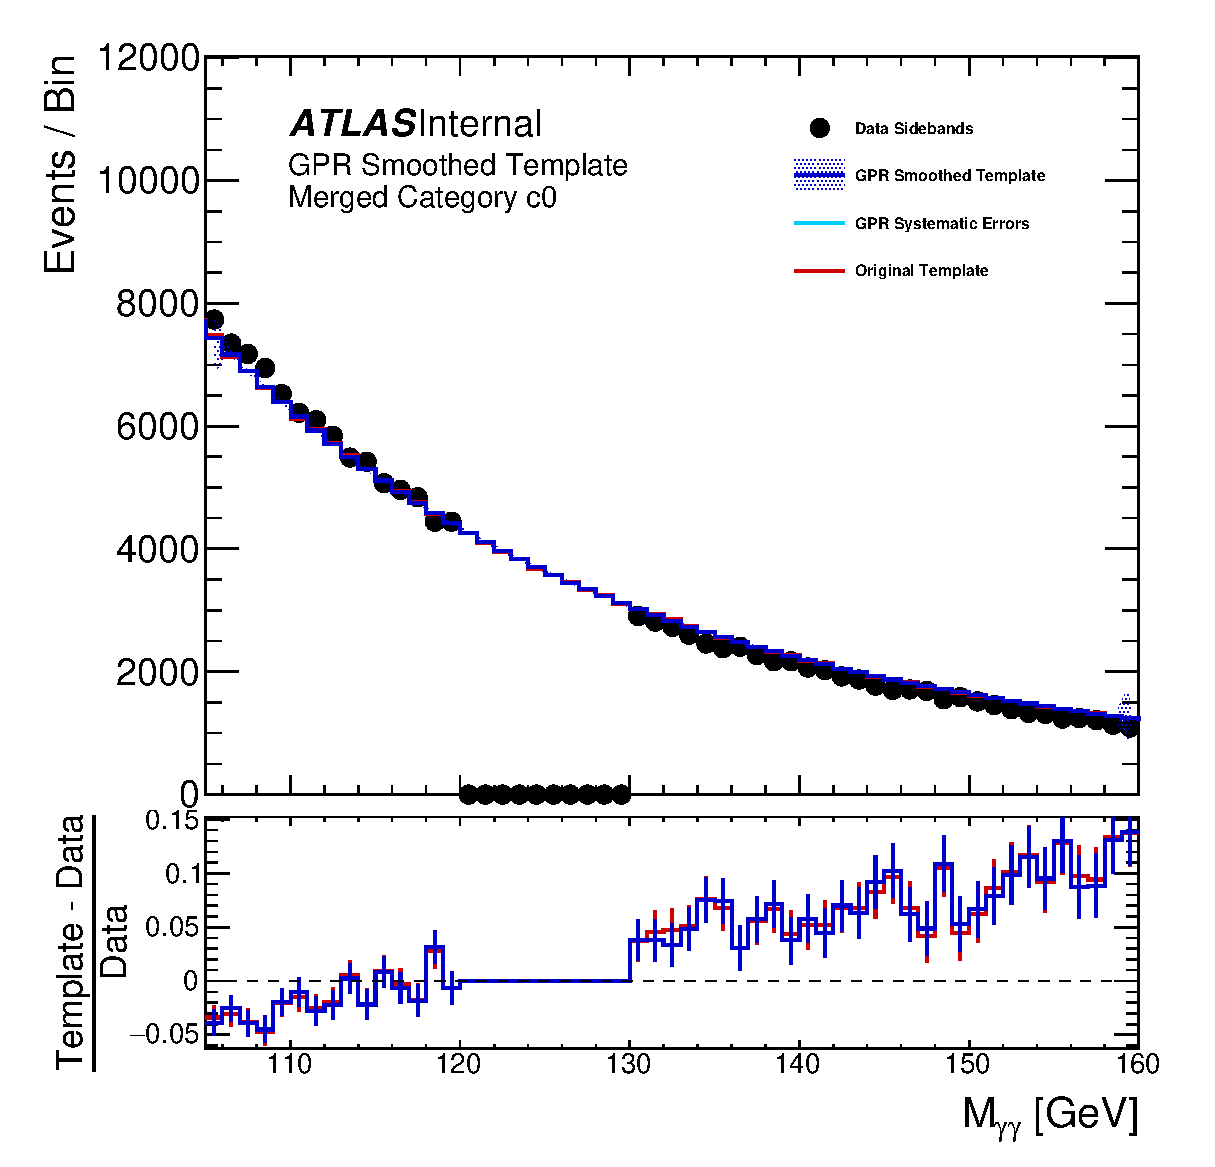
\includegraphics[width=\linewidth]{figures/background/gpr/coupCatTemplates/GPR_Smoothed_Plot_hmgg_c0.eps}
	\caption{GG2H\_0J\_PTH\_0\_10\_\_0}
\end{subfigure}
\begin{subfigure}[T]{0.49\linewidth}
	\centering
	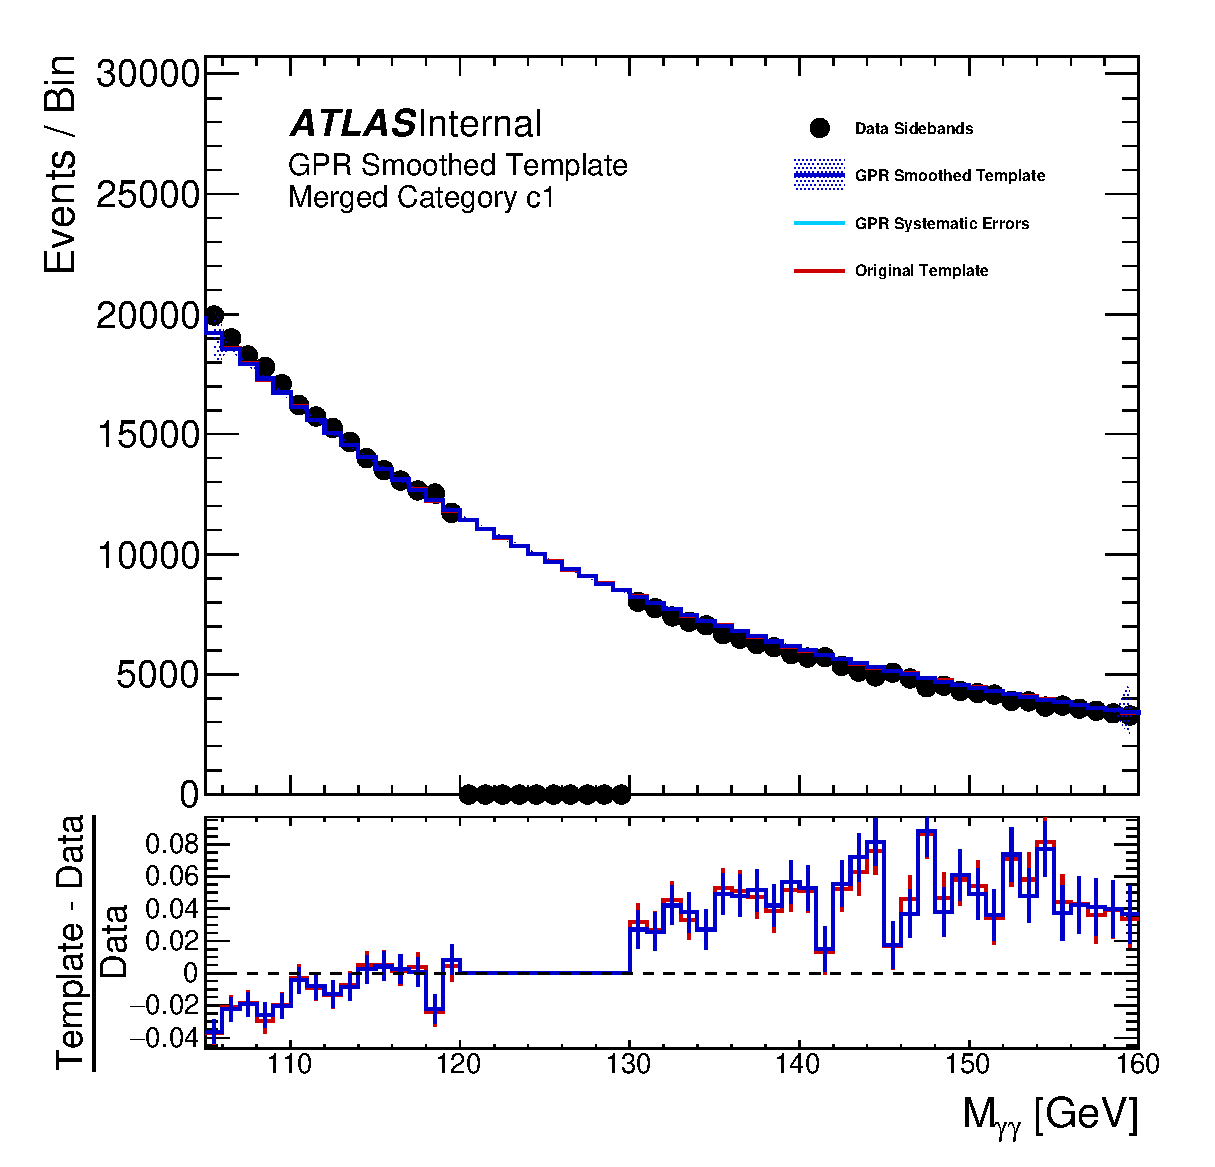
\includegraphics[width=\linewidth]{figures/background/gpr/coupCatTemplates/GPR_Smoothed_Plot_hmgg_c1.eps}
	\caption{GG2H\_0J\_PTH\_GT10\_\_0}
\end{subfigure}
\begin{subfigure}[T]{0.49\linewidth}
	\centering
	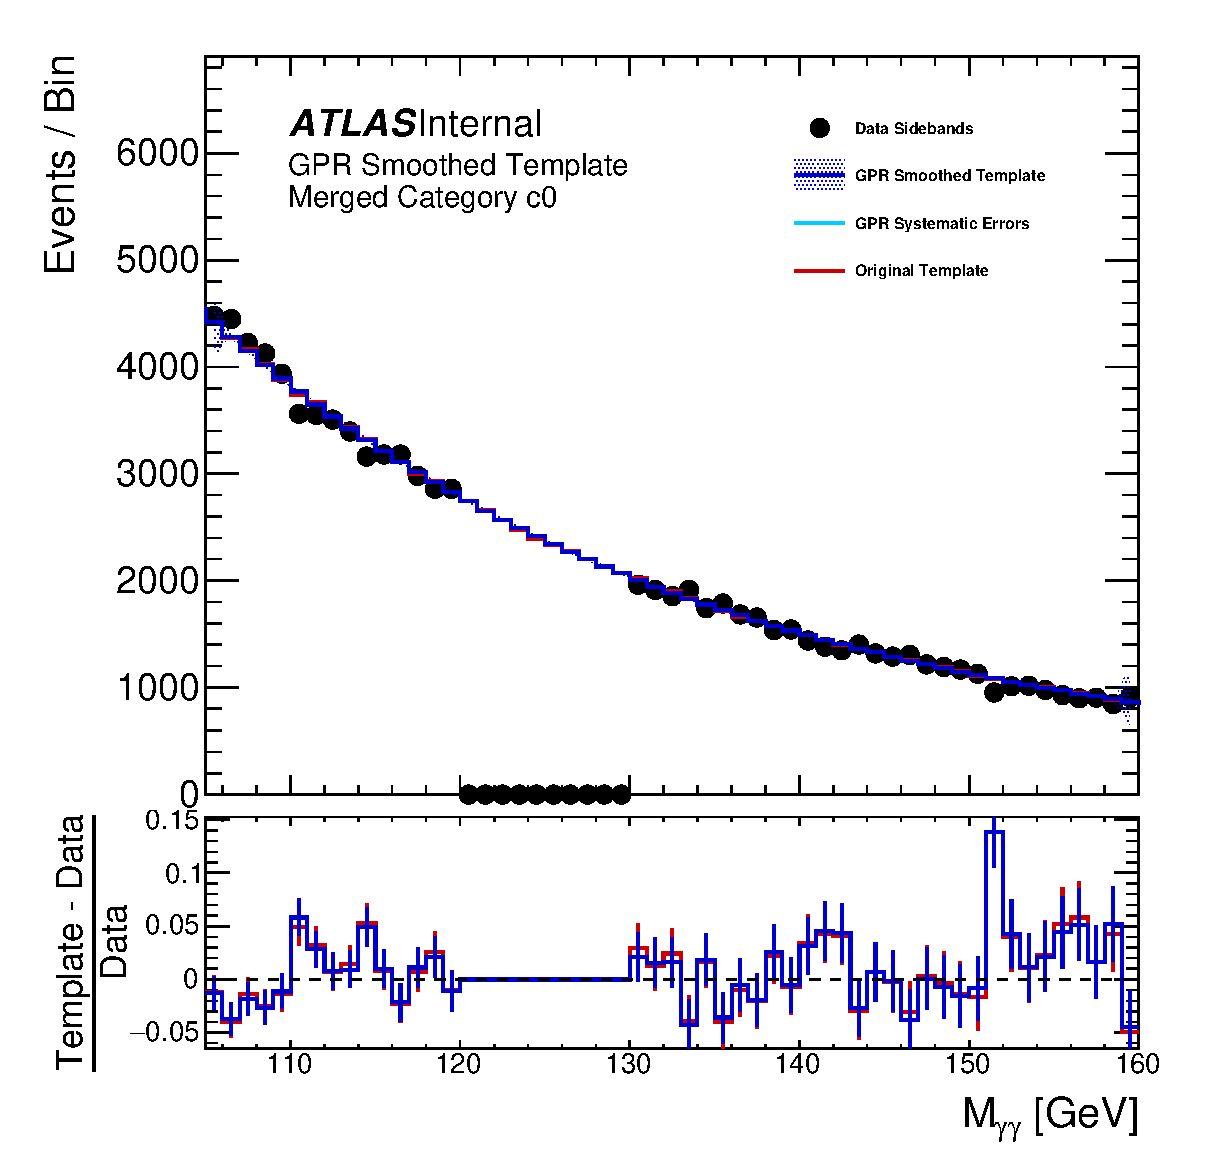
\includegraphics[width=\linewidth]{figures/background/gpr/coupCatTemplates/GPR_Smoothed_Plot_hmgg_2Merge4_c0.eps}
	\caption{GG2H\_1J\_PTH\_0\_60}
\end{subfigure}
\begin{subfigure}[T]{0.49\linewidth}
	\centering
	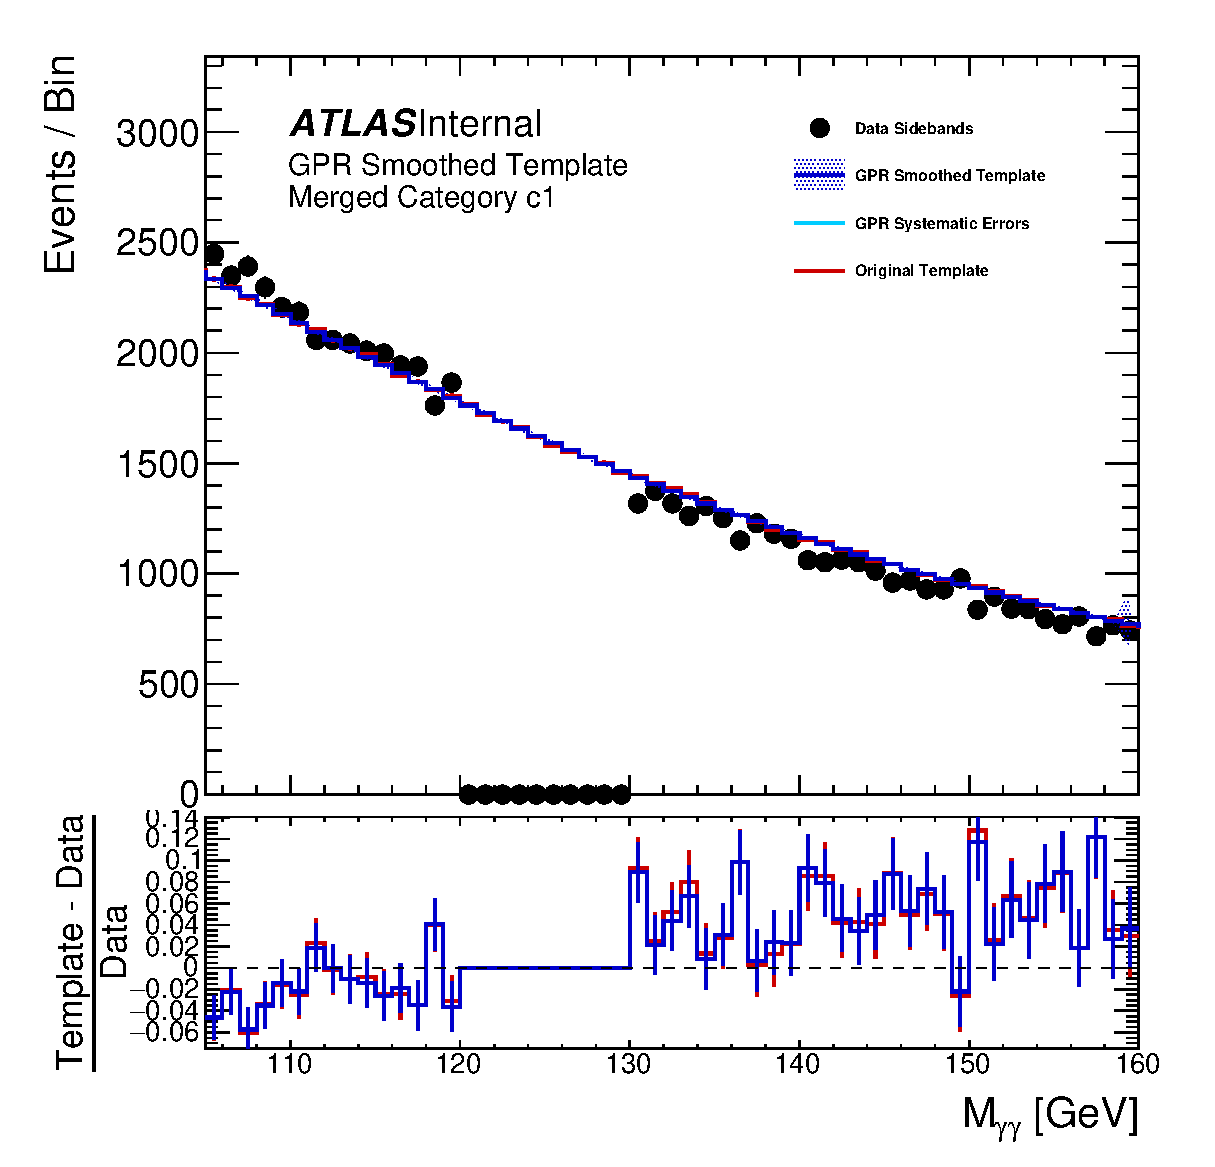
\includegraphics[width=\linewidth]{figures/background/gpr/coupCatTemplates/GPR_Smoothed_Plot_hmgg_2Merge4_c1.eps}
	\caption{GG2H\_1J\_PTH\_60\_120}
\end{subfigure}
\caption{The full Run 2 background templates of the labelled categories. The red shape shows the original background template, the blue shape shows the smoothed background template, and the black points show the data sidebands (for reference). The bottom panel shows the fractional difference between the smoothed and un-smoothed templates and the data sidebands.}
\label{fig:gpr_coupcat_1}
\end{center}
\end{figure}


\begin{figure} 
\begin{center}
\begin{subfigure}[T]{0.49\linewidth}
	\centering
	\includegraphics[width=\linewidth]{figures/background/gpr/coupCatTemplates/GPR_Smoothed_Plot_hmgg_c6.eps}
	\caption{GG2H\_1J\_PTH\_120\_200\_\_0}
\end{subfigure}
\begin{subfigure}[T]{0.49\linewidth}
	\centering
	\includegraphics[width=\linewidth]{figures/background/gpr/coupCatTemplates/GPR_Smoothed_Plot_hmgg_c7.eps}
	\caption{GG2H\_1J\_PTH\_120\_200\_\_1}
\end{subfigure}
\begin{subfigure}[T]{0.49\linewidth}
	\centering
	\includegraphics[width=\linewidth]{figures/background/gpr/coupCatTemplates/GPR_Smoothed_Plot_hmgg_c8.eps}
	\caption{GG2H\_GE2J\_MJJ\_0\_350\_PTH\_0\_60\_\_0}
\end{subfigure}
\begin{subfigure}[T]{0.49\linewidth}
	\centering
	\includegraphics[width=\linewidth]{figures/background/gpr/coupCatTemplates/GPR_Smoothed_Plot_hmgg_c9.eps}
	\caption{GG2H\_GE2J\_MJJ\_0\_350\_PTH\_0\_60\_\_1}
\end{subfigure}
\caption{The full Run~2 background templates of the labelled categories. The red shape shows the original background template, the blue shape shows the smoothed background template, and the black points show the data sidebands (for reference). The bottom panel shows the fractional difference between the smoothed and un-smoothed templates and the data sidebands. }
\label{fig:gpr_coupcat_2}
\end{center}
\end{figure}

\begin{figure} 
\begin{center}
\begin{subfigure}[T]{0.49\linewidth}
	\centering
	\includegraphics[width=\linewidth]{figures/background/gpr/coupCatTemplates/GPR_Smoothed_Plot_hmgg_c10.eps}
	\caption{GG2H\_GE2J\_MJJ\_0\_350\_PTH\_0\_60\_\_2}
\end{subfigure}
\begin{subfigure}[T]{0.49\linewidth}
	\centering
	\includegraphics[width=\linewidth]{figures/background/gpr/coupCatTemplates/GPR_Smoothed_Plot_hmgg_c11.eps}
	\caption{GG2H\_GE2J\_MJJ\_0\_350\_PTH\_60\_120\_\_0}
\end{subfigure}
\begin{subfigure}[T]{0.49\linewidth}
	\centering
	\includegraphics[width=\linewidth]{figures/background/gpr/coupCatTemplates/GPR_Smoothed_Plot_hmgg_c12.eps}
	\caption{GG2H\_GE2J\_MJJ\_0\_350\_PTH\_60\_120\_\_1}
\end{subfigure}
\begin{subfigure}[T]{0.49\linewidth}
	\centering
	\includegraphics[width=\linewidth]{figures/background/gpr/coupCatTemplates/GPR_Smoothed_Plot_hmgg_c13.eps}
	\caption{GG2H\_GE2J\_MJJ\_0\_350\_PTH\_60\_120\_\_2}
\end{subfigure}
\caption{The full Run~2 background templates of the labelled categories. The red shape shows the original background template, the blue shape shows the smoothed background template, and the black points show the data sidebands (for reference). The bottom panel shows the fractional difference between the smoothed and un-smoothed templates and the data sidebands. }
\label{fig:gpr_coupcat_3}
\end{center}
\end{figure}

\begin{figure}
\begin{center}
\begin{subfigure}[T]{0.49\linewidth}
	\centering
	\includegraphics[width=\linewidth]{figures/background/gpr/coupCatTemplates/GPR_Smoothed_Plot_hmgg_c14.eps}
	\caption{\tiny{GG2H\_GE2J\_MJJ\_0\_350\_PTH\_120\_200\_\_0}}
\end{subfigure}
\begin{subfigure}[T]{0.49\linewidth}
	\centering
	\includegraphics[width=\linewidth]{figures/background/gpr/coupCatTemplates/GPR_Smoothed_Plot_hmgg_c15.eps}
	\caption{\tiny{GG2H\_GE2J\_MJJ\_0\_350\_PTH\_120\_200\_\_1}}
\end{subfigure}
\begin{subfigure}[T]{0.49\linewidth}
	\centering
	\includegraphics[width=\linewidth]{figures/background/gpr/coupCatTemplates/GPR_Smoothed_Plot_hmgg_c16.eps}
	\caption{\tiny{GG2H\_GE2J\_MJJ\_350\_700\_PTH\_0\_200\_PTHJJ\_0\_25\_\_0}}
\end{subfigure}
\begin{subfigure}[T]{0.49\linewidth}
	\centering
	\includegraphics[width=\linewidth]{figures/background/gpr/coupCatTemplates/GPR_Smoothed_Plot_hmgg_c17.eps}
	\caption{\tiny{GG2H\_GE2J\_MJJ\_350\_700\_PTH\_0\_200\_PTHJJ\_0\_25\_\_1}}
\end{subfigure}
\caption{The full Run~2 background templates of the labelled categories. The red shape shows the original background template, the blue shape shows the smoothed background template, and the black points show the data sidebands (for reference). The bottom panel shows the fractional difference between the smoothed and un-smoothed templates and the data sidebands. }
 \label{fig:gpr_coupcat_4}
 \end{center}
\end{figure}

\begin{figure}
\begin{center}
\begin{subfigure}[T]{0.49\linewidth}
	\centering
	\includegraphics[width=\linewidth]{figures/background/gpr/coupCatTemplates/GPR_Smoothed_Plot_hmgg_c18.eps}
	\caption{\tiny{GG2H\_GE2J\_MJJ\_350\_700\_PTH\_0\_200\_PTHJJ\_0\_25\_\_2}}
\end{subfigure}
\begin{subfigure}[T]{0.49\linewidth}
	\centering
	\includegraphics[width=\linewidth]{figures/background/gpr/coupCatTemplates/GPR_Smoothed_Plot_hmgg_c19.eps}
	\caption{\tiny{GG2H\_GE2J\_MJJ\_350\_700\_PTH\_0\_200\_PTHJJ\_GT25\_\_0}}
\end{subfigure}
\begin{subfigure}[T]{0.49\linewidth}
	\centering
	\includegraphics[width=\linewidth]{figures/background/gpr/coupCatTemplates/GPR_Smoothed_Plot_hmgg_c20.eps}
	\caption{\tiny{GG2H\_GE2J\_MJJ\_350\_700\_PTH\_0\_200\_PTHJJ\_GT25\_\_1}}
\end{subfigure}
\begin{subfigure}[T]{0.49\linewidth}
	\centering
	\includegraphics[width=\linewidth]{figures/background/gpr/coupCatTemplates/GPR_Smoothed_Plot_hmgg_c21.eps}
	\caption{\tiny{GG2H\_GE2J\_MJJ\_350\_700\_PTH\_0\_200\_PTHJJ\_GT25\_\_2}}
\end{subfigure}
\caption{The full Run~2 background templates of the labelled categories. The red shape shows the original background template, the blue shape shows the smoothed background template, and the black points show the data sidebands (for reference). The bottom panel shows the fractional difference between the smoothed and un-smoothed templates and the data sidebands. }
 \label{fig:gpr_coupcat_5}
 \end{center}
\end{figure}

\begin{figure} 
\begin{center}
\begin{subfigure}[T]{0.49\linewidth}
	\centering
	\includegraphics[width=\linewidth]{figures/background/gpr/coupCatTemplates/GPR_Smoothed_Plot_hmgg_c22.eps}
	\caption{\tiny{GG2H\_GE2J\_MJJ\_GT700\_PTH\_0\_200\_PTHJJ\_0\_25\_\_0}}
\end{subfigure}
\begin{subfigure}[T]{0.49\linewidth}
	\centering
	\includegraphics[width=\linewidth]{figures/background/gpr/coupCatTemplates/GPR_Smoothed_Plot_hmgg_c23.eps}
	\caption{\tiny{GG2H\_GE2J\_MJJ\_GT700\_PTH\_0\_200\_PTHJJ\_0\_25\_\_1}}
\end{subfigure}
\begin{subfigure}[T]{0.49\linewidth}
	\centering
	\includegraphics[width=\linewidth]{figures/background/gpr/coupCatTemplates/GPR_Smoothed_Plot_hmgg_c24.eps}
	\caption{\tiny{GG2H\_GE2J\_MJJ\_GT700\_PTH\_0\_200\_PTHJJ\_0\_25\_\_2}}
\end{subfigure}
\begin{subfigure}[T]{0.49\linewidth}
	\centering
	\includegraphics[width=\linewidth]{figures/background/gpr/coupCatTemplates/GPR_Smoothed_Plot_hmgg_c25.eps}
	\caption{\tiny{GG2H\_GE2J\_MJJ\_GT700\_PTH\_0\_200\_PTHJJ\_GT25\_\_0}}
\end{subfigure}
\caption{The full Run~2 background templates of the labelled categories. The red shape shows the original background template, the blue shape shows the smoothed background template, and the black points show the data sidebands (for reference). The bottom panel shows the fractional difference between the smoothed and un-smoothed templates and the data sidebands. }
\label{fig:gpr_coupcat_6}
\end{center}
\end{figure}

\begin{figure}
\begin{center}
\begin{subfigure}[T]{0.49\linewidth}
	\centering
	\includegraphics[width=\linewidth]{figures/background/gpr/coupCatTemplates/GPR_Smoothed_Plot_hmgg_c26.eps}
	\caption{\tiny{GG2H\_GE2J\_MJJ\_GT700\_PTH\_0\_200\_PTHJJ\_GT25\_\_1}}
\end{subfigure}
\begin{subfigure}[T]{0.49\linewidth}
	\centering
	\includegraphics[width=\linewidth]{figures/background/gpr/coupCatTemplates/GPR_Smoothed_Plot_hmgg_c27.eps}
	\caption{\tiny{GG2H\_GE2J\_MJJ\_GT700\_PTH\_0\_200\_PTHJJ\_GT25\_\_2}}
\end{subfigure}
\begin{subfigure}[T]{0.49\linewidth}
	\centering
	\includegraphics[width=\linewidth]{figures/background/gpr/coupCatTemplates/GPR_Smoothed_Plot_hmgg_c28.eps}
	\caption{GG2H\_PTH\_200\_300\_\_0}
\end{subfigure}
\begin{subfigure}[T]{0.49\linewidth}
	\centering
	\includegraphics[width=\linewidth]{figures/background/gpr/coupCatTemplates/GPR_Smoothed_Plot_hmgg_c29.eps}
	\caption{GG2H\_PTH\_200\_300\_\_1}
\end{subfigure}
	\caption{The full Run~2 background templates of the labelled categories. The red shape shows the original background template, the blue shape shows the smoothed background template, and the black points show the data sidebands (for reference). The bottom panel shows the fractional difference between the smoothed and un-smoothed templates and the data sidebands. }
 \label{fig:gpr_coupcat_7}
 \end{center}
\end{figure}

\begin{figure}
\begin{center}
\begin{subfigure}[T]{0.49\linewidth}
	\centering
	\includegraphics[width=\linewidth]{figures/background/gpr/coupCatTemplates/GPR_Smoothed_Plot_hmgg_c30.eps}
	\caption{GG2H\_PTH\_200\_300\_\_2}
\end{subfigure}
%\begin{subfigure}[T]{0.49\linewidth}
%	\centering
%	\includegraphics[width=\linewidth]{figures/background/gpr/coupCatTemplates/GPR_Smoothed_Plot_hmgg_c31.eps}
%	\caption{GG2H\_PTH\_300\_450\_\_0}
%\end{subfigure}
\begin{subfigure}[T]{0.49\linewidth}
	\centering
	\includegraphics[width=\linewidth]{figures/background/gpr/coupCatTemplates/GPR_Smoothed_Plot_hmgg_c32.eps}
	\caption{GG2H\_PTH\_300\_450\_\_1}
\end{subfigure}
\begin{subfigure}[T]{0.49\linewidth}
	\centering
	\includegraphics[width=\linewidth]{figures/background/gpr/coupCatTemplates/GPR_Smoothed_Plot_hmgg_c33.eps}
	\caption{GG2H\_PTH\_300\_450\_\_2}
\end{subfigure}
	\caption{The full Run~2 background templates of the labelled categories. The red shape shows the original background template, the blue shape shows the smoothed background template, and the black points show the data sidebands (for reference). The bottom panel shows the fractional difference between the smoothed and un-smoothed templates and the data sidebands. }
 \label{fig:gpr_coupcat_8}
 \end{center}
\end{figure}

\begin{figure}
\begin{center}
%\begin{subfigure}[T]{0.49\linewidth}
%	\centering
%	\includegraphics[width=\linewidth]{figures/background/gpr/coupCatTemplates/GPR_Smoothed_Plot_hmgg_c34.eps}
%	\caption{GG2H\_PTH\_450\_650\_\_0}
%\end{subfigure}
\begin{subfigure}[T]{0.49\linewidth}
	\centering
	\includegraphics[width=\linewidth]{figures/background/gpr/coupCatTemplates/GPR_Smoothed_Plot_hmgg_c35New.eps}
	\caption{GG2H\_PTH\_450\_650\_\_1}
\end{subfigure}
%\begin{subfigure}[T]{0.49\linewidth}
%	\centering
%	\includegraphics[width=\linewidth]{figures/background/gpr/coupCatTemplates/GPR_Smoothed_Plot_hmgg_c36.eps}
%	\caption{GG2H\_PTH\_GT650\_\_0}
%\end{subfigure}
%\begin{subfigure}[T]{0.49\linewidth}
%	\centering
%	\includegraphics[width=\linewidth]{figures/background/gpr/coupCatTemplates/GPR_Smoothed_Plot_hmgg_c37.eps}
%	\caption{GG2H\_PTH\_GT650\_\_1}
%\end{subfigure}
\caption{The full Run~2 background templates of the labelled categories. The red shape shows the original background template, the blue shape shows the smoothed background template, and the black points show the data sidebands (for reference). The bottom panel shows the fractional difference between the smoothed and un-smoothed templates and the data sidebands. }
 \label{fig:gpr_coupcat_9}
 \end{center}
\end{figure}

\begin{figure}
\begin{center}
%\begin{subfigure}[T]{0.49\linewidth}
%	\centering
%	\includegraphics[width=\linewidth]{figures/background/gpr/coupCatTemplates/GPR_Smoothed_Plot_hmgg_c38.eps}
%	\caption{QQ2HQQ\_0J\_\_0}
%\end{subfigure}
\begin{subfigure}[T]{0.49\linewidth}
	\centering
	\includegraphics[width=\linewidth]{figures/background/gpr/coupCatTemplates/GPR_Smoothed_Plot_hmgg_c39.eps}
	\caption{QQ2HQQ\_0J\_\_1}
\end{subfigure}
%\begin{subfigure}[T]{0.49\linewidth}
%	\centering
%	\includegraphics[width=\linewidth]{figures/background/gpr/coupCatTemplates/GPR_Smoothed_Plot_hmgg_c40.eps}
%	\caption{QQ2HQQ\_1J\_\_0}
%\end{subfigure}
\begin{subfigure}[T]{0.49\linewidth}
	\centering
	\includegraphics[width=\linewidth]{figures/background/gpr/coupCatTemplates/GPR_Smoothed_Plot_hmgg_c41.eps}
	\caption{QQ2HQQ\_1J\_\_1}
\end{subfigure}
\caption{The full Run~2 background templates of the labelled categories. The red shape shows the original background template, the blue shape shows the smoothed background template, and the black points show the data sidebands (for reference). The bottom panel shows the fractional difference between the smoothed and un-smoothed templates and the data sidebands. }
 \label{fig:gpr_coupcat_10}
 \end{center}
\end{figure}

\begin{figure} 
\begin{center}
\begin{subfigure}[T]{0.49\linewidth}
	\centering
	\includegraphics[width=\linewidth]{figures/background/gpr/coupCatTemplates/GPR_Smoothed_Plot_hmgg_c42.eps}
	\caption{QQ2HQQ\_1J\_\_2}
\end{subfigure}
%\begin{subfigure}[T]{0.49\linewidth}
%	\centering
%	\includegraphics[width=\linewidth]{figures/background/gpr/coupCatTemplates/GPR_Smoothed_Plot_hmgg_c43.eps}
%	\caption{QQ2HQQ\_GE2J\_MJJ\_0\_60\_\_0}
%\end{subfigure}
\begin{subfigure}[T]{0.49\linewidth}
	\centering
	\includegraphics[width=\linewidth]{figures/background/gpr/coupCatTemplates/GPR_Smoothed_Plot_hmgg_c44.eps}
	\caption{QQ2HQQ\_GE2J\_MJJ\_0\_60\_\_1}
\end{subfigure}
\begin{subfigure}[T]{0.49\linewidth}
	\centering
	\includegraphics[width=\linewidth]{figures/background/gpr/coupCatTemplates/GPR_Smoothed_Plot_hmgg_c45.eps}
	\caption{QQ2HQQ\_GE2J\_MJJ\_0\_60\_\_2}
\end{subfigure}
\caption{The full Run~2 background templates of the labelled categories. The red shape shows the original background template, the blue shape shows the smoothed background template, and the black points show the data sidebands (for reference). The bottom panel shows the fractional difference between the smoothed and un-smoothed templates and the data sidebands. }
\label{fig:gpr_coupcat_11}
\end{center}
\end{figure}

\begin{figure}
\begin{center}
\begin{subfigure}[T]{0.49\linewidth}
	\centering
	\includegraphics[width=\linewidth]{figures/background/gpr/coupCatTemplates/GPR_Smoothed_Plot_hmgg_c46.eps}
	\caption{QQ2HQQ\_GE2J\_MJJ\_60\_120\_\_0}
\end{subfigure}
\begin{subfigure}[T]{0.49\linewidth}
	\centering
	\includegraphics[width=\linewidth]{figures/background/gpr/coupCatTemplates/GPR_Smoothed_Plot_hmgg_c47.eps}
	\caption{QQ2HQQ\_GE2J\_MJJ\_60\_120\_\_1}
\end{subfigure}
%\begin{subfigure}[T]{0.49\linewidth}
%	\centering
%	\includegraphics[width=\linewidth]{figures/background/gpr/coupCatTemplates/GPR_Smoothed_Plot_hmgg_c48.eps}
%	\caption{QQ2HQQ\_GE2J\_MJJ\_120\_350\_\_0}
%\end{subfigure}
\begin{subfigure}[T]{0.49\linewidth}
	\centering
	\includegraphics[width=\linewidth]{figures/background/gpr/coupCatTemplates/GPR_Smoothed_Plot_hmgg_c49.eps}
	\caption{QQ2HQQ\_GE2J\_MJJ\_120\_350\_\_1}
\end{subfigure}
\caption{The full Run~2 background templates of the labelled categories. The red shape shows the original background template, the blue shape shows the smoothed background template, and the black points show the data sidebands (for reference). The bottom panel shows the fractional difference between the smoothed and un-smoothed templates and the data sidebands. }
 \label{fig:gpr_coupcat_12}
 \end{center}
\end{figure}

\begin{figure}
\begin{center}
\begin{subfigure}[T]{0.49\linewidth}
	\centering
	\includegraphics[width=\linewidth]{figures/background/gpr/coupCatTemplates/GPR_Smoothed_Plot_hmgg_c50.eps}
	\caption{\tiny{QQ2HQQ\_GE2J\_MJJ\_120\_350\_\_2}}
\end{subfigure}
%\begin{subfigure}[T]{0.49\linewidth}
%	\centering
%	\includegraphics[width=\linewidth]{figures/background/gpr/coupCatTemplates/GPR_Smoothed_Plot_hmgg_c51.eps}
%	\caption{\tiny{QQ2HQQ\_GE2J\_MJJ\_350\_700\_PTH\_0\_200\_PTHJJ\_0\_25\_\_0}}
%\end{subfigure}
\begin{subfigure}[T]{0.49\linewidth}
	\centering
	\includegraphics[width=\linewidth]{figures/background/gpr/coupCatTemplates/GPR_Smoothed_Plot_hmgg_c52.eps}
	\caption{\tiny{QQ2HQQ\_GE2J\_MJJ\_350\_700\_PTH\_0\_200\_PTHJJ\_0\_25\_\_1}}
\end{subfigure}
%\begin{subfigure}[T]{0.49\linewidth}
%	\centering
%	\includegraphics[width=\linewidth]{figures/background/gpr/coupCatTemplates/GPR_Smoothed_Plot_hmgg_c53.eps}
%	\caption{\tiny{QQ2HQQ\_GE2J\_MJJ\_350\_700\_PTH\_0\_200\_PTHJJ\_GT25\_\_0}}
%\end{subfigure}
\caption{The full Run~2 background templates of the labelled categories. The red shape shows the original background template, the blue shape shows the smoothed background template, and the black points show the data sidebands (for reference). The bottom panel shows the fractional difference between the smoothed and un-smoothed templates and the data sidebands. }
 \label{fig:gpr_coupcat_13}
 \end{center}
\end{figure}

\begin{figure}
\begin{center}
%\begin{subfigure}[T]{0.49\linewidth}
%	\centering
%	\includegraphics[width=\linewidth]{figures/background/gpr/coupCatTemplates/GPR_Smoothed_Plot_hmgg_c54.eps}
%	\caption{\tiny{QQ2HQQ\_GE2J\_MJJ\_350\_700\_PTH\_0\_200\_PTHJJ\_GT25\_\_1}}
%\end{subfigure}
%\begin{subfigure}[T]{0.49\linewidth}
%	\centering
%	\includegraphics[width=\linewidth]{figures/background/gpr/coupCatTemplates/GPR_Smoothed_Plot_hmgg_c55.eps}
%	\caption{\tiny{QQ2HQQ\_GE2J\_MJJ\_GT700\_PTH\_0\_200\_PTHJJ\_0\_25\_\_0}}
%\end{subfigure}
\begin{subfigure}[T]{0.49\linewidth}
	\centering
	\includegraphics[width=\linewidth]{figures/background/gpr/coupCatTemplates/GPR_Smoothed_Plot_hmgg_c56.eps}
	\caption{\tiny{QQ2HQQ\_GE2J\_MJJ\_GT700\_PTH\_0\_200\_PTHJJ\_0\_25\_\_1}}
\end{subfigure}
%\begin{subfigure}[T]{0.49\linewidth}
%	\centering
%	\includegraphics[width=\linewidth]{figures/background/gpr/coupCatTemplates/GPR_Smoothed_Plot_hmgg_c57.eps}
%	\caption{\tiny{QQ2HQQ\_GE2J\_MJJ\_GT700\_PTH\_0\_200\_PTHJJ\_GT25\_\_0}}
%\end{subfigure}
\caption{The full Run~2 background templates of the labelled categories. The red shape shows the original background template, the blue shape shows the smoothed background template, and the black points show the data sidebands (for reference). The bottom panel shows the fractional difference between the smoothed and un-smoothed templates and the data sidebands. }
 \label{fig:gpr_coupcat_14}
 \end{center}
\end{figure}

\begin{figure}
\begin{center}
%\begin{subfigure}[T]{0.49\linewidth}
%	\centering
%	\includegraphics[width=\linewidth]{figures/background/gpr/coupCatTemplates/GPR_Smoothed_Plot_hmgg_c58.eps}
%	\caption{\tiny{QQ2HQQ\_GE2J\_MJJ\_GT700\_PTH\_0\_200\_PTHJJ\_GT25\_\_1}}
%\end{subfigure}
\begin{subfigure}[T]{0.49\linewidth}
	\centering
	\includegraphics[width=\linewidth]{figures/background/gpr/coupCatTemplates/GPR_Smoothed_Plot_hmgg_c59.eps}
	\caption{\tiny{QQ2HQQ\_GE2J\_MJJ\_GT700\_PTH\_0\_200\_PTHJJ\_GT25\_\_2}}
\end{subfigure}
%\begin{subfigure}[T]{0.49\linewidth}
%	\centering
%	\includegraphics[width=\linewidth]{figures/background/gpr/coupCatTemplates/GPR_Smoothed_Plot_hmgg_c60.eps}
%	\caption{\tiny{QQ2HQQ\_GE2J\_MJJ\_350\_700\_PTH\_GT200\_\_0}}
%\end{subfigure}
%\begin{subfigure}[T]{0.49\linewidth}
%	\centering
%	\includegraphics[width=\linewidth]{figures/background/gpr/coupCatTemplates/GPR_Smoothed_Plot_hmgg_c61.eps}
%	\caption{\tiny{QQ2HQQ\_GE2J\_MJJ\_350\_700\_PTH\_GT200\_\_1}}
%\end{subfigure}
\caption{The full Run~2 background templates of the labelled categories. The red shape shows the original background template, the blue shape shows the smoothed background template, and the black points show the data sidebands (for reference). The bottom panel shows the fractional difference between the smoothed and un-smoothed templates and the data sidebands. }
 \label{fig:gpr_coupcat_15}
 \end{center}
\end{figure}

\begin{figure} 
\begin{center}
%\begin{subfigure}[T]{0.49\linewidth}
%	\centering
%	\includegraphics[width=\linewidth]{figures/background/gpr/coupCatTemplates/GPR_Smoothed_Plot_hmgg_c62.eps}
%	\caption{QQ2HQQ\_GE2J\_MJJ\_GT700\_PTH\_GT200\_\_0}
%\end{subfigure}
\begin{subfigure}[T]{0.49\linewidth}
	\centering
	\includegraphics[width=\linewidth]{figures/background/gpr/coupCatTemplates/GPR_Smoothed_Plot_hmgg_c63.eps}
	\caption{QQ2HQQ\_GE2J\_MJJ\_GT700\_PTH\_GT200\_\_1}
\end{subfigure}
\begin{subfigure}[T]{0.49\linewidth}
	\centering
	\includegraphics[width=\linewidth]{figures/background/gpr/coupCatTemplates/GPR_Smoothed_Plot_hmgg_c64.eps}
	\caption{UNSELECTED\_WH}
\end{subfigure}
\begin{subfigure}[T]{0.49\linewidth}
	\centering
	\includegraphics[width=\linewidth]{figures/background/gpr/coupCatTemplates/GPR_Smoothed_Plot_hmgg_c65.eps}
	\caption{QQ2HLNU\_PTV\_0\_75\_\_0}
\end{subfigure}
\caption{The full Run~2 background templates of the labelled categories. The red shape shows the original background template, the blue shape shows the smoothed background template, and the black points show the data sidebands (for reference). The bottom panel shows the fractional difference between the smoothed and un-smoothed templates and the data sidebands. }
\label{fig:gpr_coupcat_16}
\end{center}
\end{figure}

\begin{figure}
\begin{center}
\begin{subfigure}[T]{0.49\linewidth}
	\centering
	\includegraphics[width=\linewidth]{figures/background/gpr/coupCatTemplates/GPR_Smoothed_Plot_hmgg_c66.eps}
	\caption{QQ2HLNU\_PTV\_0\_75\_\_1}
\end{subfigure}
\begin{subfigure}[T]{0.49\linewidth}
	\centering
	\includegraphics[width=\linewidth]{figures/background/gpr/coupCatTemplates/GPR_Smoothed_Plot_hmgg_c67.eps}
	\caption{QQ2HLNU\_PTV\_75\_150\_\_0}
\end{subfigure}
\begin{subfigure}[T]{0.49\linewidth}
	\centering
	\includegraphics[width=\linewidth]{figures/background/gpr/coupCatTemplates/GPR_Smoothed_Plot_hmgg_c68.eps}
	\caption{QQ2HLNU\_PTV\_75\_150\_\_1}
\end{subfigure}
\begin{subfigure}[T]{0.49\linewidth}
	\centering
	\includegraphics[width=\linewidth]{figures/background/gpr/coupCatTemplates/GPR_Smoothed_Plot_hmgg_c69.eps}
	\caption{QQ2HLNU\_PTV\_150\_250\_0J\_\_0}
\end{subfigure}
\caption{The full Run~2 background templates of the labelled categories. The red shape shows the original background template, the blue shape shows the smoothed background template, and the black points show the data sidebands (for reference). The bottom panel shows the fractional difference between the smoothed and un-smoothed templates and the data sidebands. }
 \label{fig:gpr_coupcat_17}
 \end{center}
\end{figure}

\begin{figure}
\begin{center}
\begin{subfigure}[T]{0.49\linewidth}
	\centering
	\includegraphics[width=\linewidth]{figures/background/gpr/coupCatTemplates/GPR_Smoothed_Plot_hmgg_c70.eps}
	\caption{QQ2HLNU\_PTV\_150\_250\_GE1J\_\_0}
\end{subfigure}
\begin{subfigure}[T]{0.49\linewidth}
	\centering
	\includegraphics[width=\linewidth]{figures/background/gpr/coupCatTemplates/GPR_Smoothed_Plot_hmgg_c71.eps}
	\caption{QQ2HLNU\_PTV\_GT250\_\_0}
\end{subfigure}
\begin{subfigure}[T]{0.49\linewidth}
	\centering
	\includegraphics[width=\linewidth]{figures/background/gpr/coupCatTemplates/GPR_Smoothed_Plot_hmgg_c72.eps}
	\caption{UNSELECTED\_ZH}
\end{subfigure}
\begin{subfigure}[T]{0.49\linewidth}
	\centering
	\includegraphics[width=\linewidth]{figures/background/gpr/coupCatTemplates/GPR_Smoothed_Plot_hmgg_c73.eps}
	\caption{HLL\_PTV\_0\_75\_\_0}
\end{subfigure}
\caption{The full Run~2 background templates of the labelled categories. The red shape shows the original background template, the blue shape shows the smoothed background template, and the black points show the data sidebands (for reference). The bottom panel shows the fractional difference between the smoothed and un-smoothed templates and the data sidebands. }
 \label{fig:gpr_coupcat_18}
 \end{center}
\end{figure}

\begin{figure}
\begin{center}
\begin{subfigure}[T]{0.49\linewidth}
	\centering
	\includegraphics[width=\linewidth]{figures/background/gpr/coupCatTemplates/GPR_Smoothed_Plot_hmgg_c74.eps}
	\caption{HLL\_PTV\_75\_150\_\_0}
\end{subfigure}
\begin{subfigure}[T]{0.49\linewidth}
	\centering
	\includegraphics[width=\linewidth]{figures/background/gpr/coupCatTemplates/GPR_Smoothed_Plot_hmgg_c75.eps}
	\caption{HLL\_PTV\_75\_150\_\_1}
\end{subfigure}
\begin{subfigure}[T]{0.49\linewidth}
	\centering
	\includegraphics[width=\linewidth]{figures/background/gpr/coupCatTemplates/GPR_Smoothed_Plot_hmgg_c76.eps}
	\caption{HLL\_PTV\_150\_250\_0J\_\_0}
\end{subfigure}
\begin{subfigure}[T]{0.49\linewidth}
	\centering
	\includegraphics[width=\linewidth]{figures/background/gpr/coupCatTemplates/GPR_Smoothed_Plot_hmgg_c77.eps}
	\caption{HLL\_PTV\_150\_250\_GE1J\_\_0}
\end{subfigure}
\caption{The full Run~2 background templates of the labelled categories. The red shape shows the original background template, the blue shape shows the smoothed background template, and the black points show the data sidebands (for reference). The bottom panel shows the fractional difference between the smoothed and un-smoothed templates and the data sidebands. }
 \label{fig:gpr_coupcat_19}
 \end{center}
\end{figure}

\begin{figure}
\begin{center}
\begin{subfigure}[T]{0.49\linewidth}
	\centering
	\includegraphics[width=\linewidth]{figures/background/gpr/coupCatTemplates/GPR_Smoothed_Plot_hmgg_c78.eps}
	\caption{HLL\_PTV\_GT250\_\_0}
\end{subfigure}
\begin{subfigure}[T]{0.49\linewidth}
	\centering
	\includegraphics[width=\linewidth]{figures/background/gpr/coupCatTemplates/GPR_Smoothed_Plot_hmgg_c79.eps}
	\caption{UNSELECTED\_TOP}
\end{subfigure}
\begin{subfigure}[T]{0.49\linewidth}
	\centering
	\includegraphics[width=\linewidth]{figures/background/gpr/coupCatTemplates/GPR_Smoothed_Plot_hmgg_c80.eps}
	\caption{TTH\_PTH\_0\_60\_\_0}
\end{subfigure}
\begin{subfigure}[T]{0.49\linewidth}
	\centering
	\includegraphics[width=\linewidth]{figures/background/gpr/coupCatTemplates/GPR_Smoothed_Plot_hmgg_c81.eps}
	\caption{TTH\_PTH\_0\_60\_\_1}
\end{subfigure}
\caption{The full Run~2 background templates of the labelled categories. The red shape shows the original background template, the blue shape shows the smoothed background template, and the black points show the data sidebands (for reference). The bottom panel shows the fractional difference between the smoothed and un-smoothed templates and the data sidebands. }
 \label{fig:gpr_coupcat_20}
 \end{center}
\end{figure}

\begin{figure} 
\begin{center}
\begin{subfigure}[T]{0.49\linewidth}
	\centering
	\includegraphics[width=\linewidth]{figures/background/gpr/coupCatTemplates/GPR_Smoothed_Plot_hmgg_c82.eps}
	\caption{TTH\_PTH\_60\_120\_\_0}
\end{subfigure}
\begin{subfigure}[T]{0.49\linewidth}
	\centering
	\includegraphics[width=\linewidth]{figures/background/gpr/coupCatTemplates/GPR_Smoothed_Plot_hmgg_c83.eps}
	\caption{TTH\_PTH\_60\_120\_\_1}
\end{subfigure}
\begin{subfigure}[T]{0.49\linewidth}
	\centering
	\includegraphics[width=\linewidth]{figures/background/gpr/coupCatTemplates/GPR_Smoothed_Plot_hmgg_c84.eps}
	\caption{TTH\_PTH\_120\_200\_\_0}
\end{subfigure}
\begin{subfigure}[T]{0.49\linewidth}
	\centering
	\includegraphics[width=\linewidth]{figures/background/gpr/coupCatTemplates/GPR_Smoothed_Plot_hmgg_c85.eps}
	\caption{TTH\_PTH\_120\_200\_\_1}
\end{subfigure}
\caption{The full Run~2 background templates of the labelled categories. The red shape shows the original background template, the blue shape shows the smoothed background template, and the black points show the data sidebands (for reference). The bottom panel shows the fractional difference between the smoothed and un-smoothed templates and the data sidebands. }
\label{fig:gpr_coupcat_21}
\end{center}
\end{figure}

\begin{figure}
\begin{center}
\begin{subfigure}[T]{0.49\linewidth}
	\centering
	\includegraphics[width=\linewidth]{figures/background/gpr/coupCatTemplates/GPR_Smoothed_Plot_hmgg_c86.eps}
	\caption{TTH\_PTH\_200\_300\_\_0}
\end{subfigure}
\begin{subfigure}[T]{0.49\linewidth}
	\centering
	\includegraphics[width=\linewidth]{figures/background/gpr/coupCatTemplates/GPR_Smoothed_Plot_hmgg_c87.eps}
	\caption{TTH\_PTH\_GT300\_\_0}
\end{subfigure}
\begin{subfigure}[T]{0.49\linewidth}
	\centering
	\includegraphics[width=\linewidth]{figures/background/gpr/coupCatTemplates/GPR_Smoothed_Plot_hmgg_c88.eps}
	\caption{THJB\_\_0}
\end{subfigure}
\begin{subfigure}[T]{0.49\linewidth}
	\centering
	\includegraphics[width=\linewidth]{figures/background/gpr/coupCatTemplates/GPR_Smoothed_Plot_hmgg_c89.eps}
	\caption{TWH\_\_0}
\end{subfigure}
\caption{The full Run~2 background templates of the labelled categories. The red shape shows the original background template, the blue shape shows the smoothed background template, and the black points show the data sidebands (for reference). The bottom panel shows the fractional difference between the smoothed and un-smoothed templates and the data sidebands. }
 \label{fig:gpr_coupcat_22}
 \end{center}
\end{figure}

\subsection{Spurious Signal GPR-smoothed templates}
\label{ssec:GPR_SS}

The SS test was completely re-run with the templates reported in \Figrange{\ref{fig:gpr_coupcat_1}}{\ref{fig:gpr_coupcat_22}}. 
We report two sets of results - first, we record the spurious signal extracted from the smoothed templates using the functional form chosen from performing the relaxed spurious signal test on the unsmoothed templates. The results are reported in \Tab{\ref{tab:spurious_sig_gp}} and \Tab{\ref{tab:spurious_sig_gp2}}. A comparison with the nominal un-smoothed SS test {reported in \Sect{\ref{ssec:bck_results}}} is presented in \Tab{\ref{tab:comp_smooth_unsmooth1}} and \Tab{\ref{tab:comp_smooth_unsmooth2}}.

Second, we record the spurious signal from the smoothed templates using the functional form chosen from performing a non-relaxed spurious signal test on the smoothed templates only (that is, removing the potential two-sigma fluctuation). The results are reported in \Tab{\ref{tab:spurious_sig_gp_tight}} and \Tab{\ref{tab:spurious_sig_gptight2}}. A comparison with the nominal un-smoothed SS test {reported in \Sect{\ref{ssec:bck_results}}} showing the choice of functional form and extracted SS is presented in \Tab{\ref{tab:comp_smooth_unsmoothtight1}} and \Tab{\ref{tab:comp_smooth_unsmoothtight2}}.

In categories where GPR is deemed unreliable due to low statistics, we put an N/A rather than numerical values. 

\begin{table}[!h]
   \centering  \scriptsize
\resizebox{\linewidth}{!}{
    \begin{tabular}{llccccccS[table-format = 3.2, round-mode = places, round-precision = 2]}
    \hline
    \hline
Event category               & Func &  $P(\chi^2)$ ($\%$) & max S  & $\frac{S}{\delta S}$ ($\%$)  &  $\frac{\zeta}{\delta S}$ ($\%$)   & $\frac{S}{S_{ref}}$ ($\%$) & $\frac{\zeta}{S_{ref}}$ ($\%$) & {MCStatUnc(\%)} \\ \hline
GG2H\_0J\_PTH\_0\_10\_\_0 & ExpPoly2 &100&-69.7&-37.4&0&-8.69&0&0.49530548967884\\
GG2H\_0J\_PTH\_GT10\_\_0 & ExpPoly2 &100&-35.4&-9.56&0&-1.47&0&0.670009490397378\\
GG2H\_1J\_PTH\_0\_60 & ExpPoly2 &100&-36.4&-25.8&0&-5.99&0&0.698428012912491\\
GG2H\_1J\_PTH\_60\_120 & ExpPoly2 &100&33.6&27.2&0&6.41&0&0.631736064193819\\
GG2H\_1J\_PTH\_120\_200\_\_0 & ExpPoly2 &100&1.36&7.49&0&3.31&0&0.390551531895638\\
GG2H\_1J\_PTH\_120\_200\_\_1 & Pow &99.7&-12.1&-45.7&-8.48&-22.4&-4.26&0.580602918054916\\
GG2H\_GE2J\_MJJ\_0\_350\_PTH\_0\_60\_\_0 & ExpPoly2 &100&-0.819&-2.04&0&-2.54&0&2.7023955135943\\
GG2H\_GE2J\_MJJ\_0\_350\_PTH\_0\_60\_\_1 & ExpPoly2 &100&19.1&21.1&0&14.4&0&0.411336805838221\\
GG2H\_GE2J\_MJJ\_0\_350\_PTH\_0\_60\_\_2 & ExpPoly2 &100&-42.7&-25.4&0&-7.84&0&0.429508103868366\\
GG2H\_GE2J\_MJJ\_0\_350\_PTH\_60\_120\_\_0 & ExpPoly2 &100&-0.136&56.9&14.8&29.4&7.56&0.385488161063533\\
GG2H\_GE2J\_MJJ\_0\_350\_PTH\_60\_120\_\_1 & ExpPoly2 &100&-2.76&-5.08&0&-2.6&0&15.4615937730169\\
  GG2H\_GE2J\_MJJ\_0\_350\_PTH\_60\_120\_\_2 & Exp &100&26.2&26.9&0&10.3&0&0.654336521469797\\
GG2H\_GE2J\_MJJ\_0\_350\_PTH\_120\_200\_\_0 & ExpPoly2 &100&0.222&1.29&0&0.555&0&0.455009822520886\\
  GG2H\_GE2J\_MJJ\_0\_350\_PTH\_120\_200\_\_1 & Pow &100&-8.76&-28&0&-11.5&0&1.14482296405002\\
  GG2H\_GE2J\_MJJ\_350\_700\_PTH\_0\_200\_PTHJJ\_0\_25\_\_0 & Pow &100&0.275&6.23&0&6.39&0&16.9005652455781\\
 GG2H\_GE2J\_MJJ\_350\_700\_PTH\_0\_200\_PTHJJ\_0\_25\_\_1 & Exp &100&1.18&9.74&0&7.1&0&1.62420586157772\\
 GG2H\_GE2J\_MJJ\_350\_700\_PTH\_0\_200\_PTHJJ\_0\_25\_\_2 & Exp &100&-3.04&-14.9&0&-16.9&0&0.915447583897439\\
 GG2H\_GE2J\_MJJ\_350\_700\_PTH\_0\_200\_PTHJJ\_GT25\_\_0 & Exp &100&0.559&8.07&0&9.4&0&6.45531622570627\\
 GG2H\_GE2J\_MJJ\_350\_700\_PTH\_0\_200\_PTHJJ\_GT25\_\_1 & ExpPoly2 &100&0.395&1.97&0&2.26&0&0.661159498041603\\
 GG2H\_GE2J\_MJJ\_350\_700\_PTH\_0\_200\_PTHJJ\_GT25\_\_2 & Exp &100&-8.92&-27.3&0&-36.2&0&0.871206318335165\\
 GG2H\_GE2J\_MJJ\_GT700\_PTH\_0\_200\_PTHJJ\_0\_25\_\_0 & Exp* &100&-0.0917&1.5&0&1.22&0&7.49501598864758\\
 GG2H\_GE2J\_MJJ\_GT700\_PTH\_0\_200\_PTHJJ\_0\_25\_\_1 & Exp &100&0.784&10.6&0&4.88&0&1.43198234521859\\
 GG2H\_GE2J\_MJJ\_GT700\_PTH\_0\_200\_PTHJJ\_0\_25\_\_2 & Pow &100&-0.896&-6.45&0&-5.65&0&11.9026015272899\\
 GG2H\_GE2J\_MJJ\_GT700\_PTH\_0\_200\_PTHJJ\_GT25\_\_0 & Pow &100&0.809&12.9&0&13.6&0&2.59876084138453\\
 GG2H\_GE2J\_MJJ\_GT700\_PTH\_0\_200\_PTHJJ\_GT25\_\_1 & Exp &100&2.08&15.1&0&13.4&0&1.12641493611108\\
 GG2H\_GE2J\_MJJ\_GT700\_PTH\_0\_200\_PTHJJ\_GT25\_\_2 & Pow &100&3.39&14.8&0&19.2&0&0.836937308150097\\
 GG2H\_PTH\_200\_300\_\_0 & Exp* &100&0.714&18.9&0&8.7&0&0.957252494113587\\
 GG2H\_PTH\_200\_300\_\_1 & Exp &100&1.76&17.7&0&5.63&0&0.963498763874657\\
 GG2H\_PTH\_200\_300\_\_2 & Pow &100&1.07&7&0&3.99&0&6.08402670298877\\
 GG2H\_PTH\_300\_450\_\_0 &N/A&N/A&N/A&N/A&N/A&N/A&N/A&1.06852533448614\\
 GG2H\_PTH\_300\_450\_\_1 &Pow*&100&0.137&3.88&0&1.69&0&4.80093522232552\\
 GG2H\_PTH\_300\_450\_\_2 & Pow &100&0.851&10.2&0&4.61&0&6.12616876624667\\
 GG2H\_PTH\_450\_650\_\_0 &N/A&N/A&N/A&N/A&N/A&N/A&N/A&4.09507019357757\\
 GG2H\_PTH\_450\_650\_\_1 & Exp* &100&0.0262&0.906&0&1.25&0&114.438450165829\\
 GG2H\_PTH\_GT650\_\_0 &N/A&N/A&N/A&N/A&N/A&N/A&N/A&9.31519538674586\\
 GG2H\_PTH\_GT650\_\_1 &N/A&N/A&N/A&N/A&N/A&N/A&N/A&20.5008019152994\\
    \hline
      \hline
      \end{tabular}
}
      \caption{
The final background modelling decision and the size of spurious signal uncertainties. The reported number here is the base SS yield, without the bias uncertainty applied; the spurious signal with the bias is used in \ref{tab:comp_smooth_unsmooth1} and \ref{tab:comp_smooth_unsmooth2}.
   In the mass range 120 GeV to 130 GeV, $S$ is the maximum fitted spurious signal yield, $\delta S$ is the associated uncertainty on the data, and $S_{ref}$ is the expected size of Higgs signal events.
   The $\zeta$ is the maximum fitted spurious signal yield which is accommodate to $2\sigma$ statistical fluctuation of the background templates.
   The "*" in the function name indicates for which categories the "low-statistic" configuration of the SS fits (different in range and initial values) was run. Like the nominal case, we require $P(\chi^2) > 1\%$. The stat uncertainty quoted is the uncertainty on the template due to Monte Carlo statistics. The functional form is chosen using a relaxed spurious signal test applied to the unsmoothed templates.
      \label{tab:spurious_sig_gp} }
\end{table}


\begin{table}[!h]
   \centering
\resizebox{\linewidth}{!}{
    \begin{tabular}{llccccccS[table-format = 3.2, round-mode = places, round-precision = 2]}
    \hline
    \hline
   Event category               & Func &  $P(\chi^2)$ ($\%$) & max S  & $\frac{S}{\delta S}$ ($\%$)  &  $\frac{\zeta}{\delta S}$ ($\%$)   & $\frac{S}{S_{ref}}$ ($\%$) & $\frac{\zeta}{S_{ref}}$ ($\%$) & {MCStatUnc(\%)} \\ \hline
    \hline
QQ2HQQ\_0J\_\_0 &N/A&N/A&N/A&N/A&N/A&N/A&N/A&1.33966217711132\\
 QQ2HQQ\_0J\_\_1 & Exp* &100&-0.204&-5.8&0&-32.8&0&1.72347584142509\\
 QQ2HQQ\_1J\_\_0 &N/A&N/A&N/A&N/A&N/A&N/A&N/A&10.0111767833968\\
 QQ2HQQ\_1J\_\_1 & Exp* &99.4&0.247&9.72&0&9.17&0&1.90419965075391\\
 QQ2HQQ\_1J\_\_2 & Pow &100&-0.67&-10.8&0&-12.5&0&-7.78847438884904\\
 QQ2HQQ\_GE2J\_MJJ\_0\_60\_\_0 &N/A&N/A&N/A&N/A&N/A&N/A&N/A&7.21481967721796\\
 QQ2HQQ\_GE2J\_MJJ\_0\_60\_\_1 & Exp* &100&-0.0541&-1.71&0&-2.64&0&2.29694236645103\\
 QQ2HQQ\_GE2J\_MJJ\_0\_60\_\_2 & Exp &100&0.221&2.64&0&4.08&0&2.63882158243597\\
 QQ2HQQ\_GE2J\_MJJ\_60\_120\_\_0 & Exp* &100&0.0616&2.17&0&1.2&0&1.8080048045713\\
 QQ2HQQ\_GE2J\_MJJ\_60\_120\_\_1 & Pow &100&0.216&3.46&0&3.2&0&3.36640567629163\\
 QQ2HQQ\_GE2J\_MJJ\_120\_350\_\_0 &N/A&N/A&N/A&N/A&N/A&N/A&N/A&3.7899430709679\\
 QQ2HQQ\_GE2J\_MJJ\_120\_350\_\_1 & Exp &100&0.971&8.82&0&6.49&0&1.76065594968039\\
 QQ2HQQ\_GE2J\_MJJ\_120\_350\_\_2 & Pow &100&2.75&13.2&0&9.22&0&1.06704675452711\\
 QQ2HQQ\_GE2J\_MJJ\_350\_700\_PTH\_0\_200\_PTHJJ\_0\_25\_\_0 &N/A&N/A&N/A&N/A&N/A&N/A&N/A&-5.40684680252816\\
 QQ2HQQ\_GE2J\_MJJ\_350\_700\_PTH\_0\_200\_PTHJJ\_0\_25\_\_1 & Exp &100&0.36&4.32&0&3.24&0&-4.97481841458847\\
 QQ2HQQ\_GE2J\_MJJ\_350\_700\_PTH\_0\_200\_PTHJJ\_GT25\_\_0 &N/A&N/A&N/A&N/A&N/A&N/A&N/A&5.19652461574041\\
 QQ2HQQ\_GE2J\_MJJ\_350\_700\_PTH\_0\_200\_PTHJJ\_GT25\_\_1 &N/A&N/A&N/A&N/A&N/A&N/A&N/A&6.50867627281213\\
 QQ2HQQ\_GE2J\_MJJ\_GT700\_PTH\_0\_200\_PTHJJ\_0\_25\_\_0 &N/A&N/A&N/A&N/A&N/A&N/A&N/A&26.9355050304416\\
 QQ2HQQ\_GE2J\_MJJ\_GT700\_PTH\_0\_200\_PTHJJ\_0\_25\_\_1 & Pow &100&0.802&5.55&0&1.7&0&2.26073174674163\\
 QQ2HQQ\_GE2J\_MJJ\_GT700\_PTH\_0\_200\_PTHJJ\_GT25\_\_0 &N/A&N/A&N/A&N/A&N/A&N/A&N/A&-120.215985009797\\
 QQ2HQQ\_GE2J\_MJJ\_GT700\_PTH\_0\_200\_PTHJJ\_GT25\_\_1 &N/A&N/A&N/A&N/A&N/A&N/A&N/A&7.77794197339088\\
 QQ2HQQ\_GE2J\_MJJ\_GT700\_PTH\_0\_200\_PTHJJ\_GT25\_\_2 & Exp &100&0.953&19.7&0&13.1&0&1.47753488916779\\
 QQ2HQQ\_GE2J\_MJJ\_350\_700\_PTH\_GT200\_\_0 &N/A&N/A&N/A&N/A&N/A&N/A&N/A&-112.614568185856\\
 QQ2HQQ\_GE2J\_MJJ\_350\_700\_PTH\_GT200\_\_1 &N/A&N/A&N/A&N/A&N/A&N/A&N/A&-3.40872856286302\\
 QQ2HQQ\_GE2J\_MJJ\_GT700\_PTH\_GT200\_\_0 &N/A&N/A&N/A&N/A&N/A&N/A&N/A&-7.85015113108702\\
 QQ2HQQ\_GE2J\_MJJ\_GT700\_PTH\_GT200\_\_1 & Exp* &100&0.199&5.73&0&2.78&0&2.05514415642155\\
 UNSELECTED\_WH & Exp &100&-1.01&-6.68&0&-12.7&0&-1.37061152325468\\
 QQ2HLNU\_PTV\_0\_75\_\_0 & Exp* &100&0.583&2.76&0&2.52&0&2.45819231639961\\
 QQ2HLNU\_PTV\_0\_75\_\_1 & Exp &100&-0.152&-2.01&0&-2.44&0&-3.79805750605463\\
 QQ2HLNU\_PTV\_75\_150\_\_0 & Exp* &100&-0.00665&-0.351&0&-0.177&0&-14.0706761236901\\
 QQ2HLNU\_PTV\_75\_150\_\_1 & Exp* &100&0.122&4.78&0&9.35&0&0.822904538511033\\
 QQ2HLNU\_PTV\_150\_250\_0J\_\_0 & Exp* &100&0.0655&4.15&0&3.54&0&3.29187007219393\\
 QQ2HLNU\_PTV\_150\_250\_GE1J\_\_0 & Exp* &100&0.0461&2.77&0&2&0&3.13035237475937\\
 QQ2HLNU\_PTV\_GT250\_\_0 & Exp* &100&0.0123&1.12&0&0.835&0&3.23202444576061\\
 UNSELECTED\_ZH & Exp &100&4.25&21.7&0&34.9&0&1.48464947491563\\
 HLL\_PTV\_0\_75\_\_0 & Exp* &100&-0.0253&-1.85&0&-2.85&0&6.89171353462766\\
 HLL\_PTV\_75\_150\_\_0 & Exp* &14.8&0.236&11.5&0&6.75&0&3.21032776840103\\
 HLL\_PTV\_75\_150\_\_1 & Exp &100&1.28&22.3&0&20.3&0&1.20370159958952\\
 HLL\_PTV\_150\_250\_0J\_\_0 & Exp* &100&0.291&18.4&0&16.2&0&1.74865906882582\\
 HLL\_PTV\_150\_250\_GE1J\_\_0 & Exp* &100&-0.00609&-0.328&0&-0.363&0&3.54907145905387\\
 HLL\_PTV\_GT250\_\_0 & Exp* &100&0.0515&3.43&0&3.14&0&3.30940326250071\\
 UNSELECTED\_TOP & Exp &100&1.99&17.1&0&16&0&1.14068598510553\\
 TTH\_PTH\_0\_60\_\_0 & Exp* &100&-0.0813&-3.23&0&-2.5&0&-2.99016467131789\\
 TTH\_PTH\_0\_60\_\_1 & Exp* &100&-0.138&-2.81&0&-4.09&0&-3.0247825646843\\
 TTH\_PTH\_60\_120\_\_0 & Exp* &100&-0.0321&-1.2&0&-0.653&0&2.07790685078307\\
 TTH\_PTH\_60\_120\_\_1 & Exp* &100&0.329&8.65&0&8.21&0&0.859211641913528\\
 TTH\_PTH\_120\_200\_\_0 & Exp* &100&0.0593&2.35&0&1.02&0&1.59274704937991\\
 TTH\_PTH\_120\_200\_\_1 & Exp* &100&0.195&5.6&0&6.61&0&2.17974966708387\\
 TTH\_PTH\_200\_300\_\_0 & Exp* &100&0.393&2.56&0&0.884&0&2.99104526173778\\
 TTH\_PTH\_GT300\_\_0 & Exp* &100&0.00755&0.562&0&0.181&0&-174.486526485406\\
 THJB\_\_0 & Exp* &100&0.055&3.05&0&7.09&0&1.28325108375627\\
 TWH\_\_0 & Exp* &100&-0.0481&-2.74&0&-5.6&0&-1.7571100311547\\
       \hline
      \hline
      \end{tabular}
}
      \caption{
The final background modelling decision and the size of spurious signal uncertainties. The reported number here is the base SS yield, without the bias uncertainty applied; the spurious signal with the bias is used in \ref{tab:comp_smooth_unsmooth1} and \ref{tab:comp_smooth_unsmooth2}.
   In the mass range 120 GeV to 130 GeV, $S$ is the maximum fitted spurious signal yield, $\delta S$ is the associated uncertainty on the data, and $S_{ref}$ is the expected size of Higgs signal events.
   The $\zeta$ is the maximum fitted spurious signal yield which is accommodate to $2\sigma$ statistical fluctuation of the background templates.
   The "*" in the function name indicates for which categories the "low-statistic" configuration of the SS fits (different in range and initial values) was run.
   Like the nominal case, we require $P(\chi^2) > 1\%$. The stat uncertainty quoted is the uncertainty on the template due to Monte Carlo statistics. The functional form is chosen using a relaxed spurious signal test applied to the unsmoothed templates. 
   \label{tab:spurious_sig_gp2}   }   
\end{table}

\begin{table}[!h]
	\centering  \scriptsize
	\resizebox{\linewidth}{!}{
		\begin{tabular}{llcc}
			\hline\hline
			                                                          & Function    & \multicolumn{2}{c}{$max(S)$} \\ 
			Event category                                            &       & Nominal  & Smooth temp \\ 
			\hline\hline
			GG2H\_0J\_PTH\_0\_10\_\_0                                 & ExpPoly2 &-117&-69.7\\
			GG2H\_0J\_PTH\_GT10\_\_0                                  & ExpPoly2 &-199&-35.4\\
			GG2H\_1J\_PTH\_0\_60                                      & ExpPoly2 &-67.1&-36.4\\
			GG2H\_1J\_PTH\_60\_120                                    & ExpPoly2 &28.7&33.6\\
			GG2H\_1J\_PTH\_120\_200\_\_0                              & ExpPoly2 &-1.79&1.36\\
			GG2H\_1J\_PTH\_120\_200\_\_1                              & Pow &-11.7&-12.1\\
			GG2H\_GE2J\_MJJ\_0\_350\_PTH\_0\_60\_\_0                  & ExpPoly2 &6.54&-0.819\\
			GG2H\_GE2J\_MJJ\_0\_350\_PTH\_0\_60\_\_1                  & ExpPoly2 &21.4&19.1\\
			GG2H\_GE2J\_MJJ\_0\_350\_PTH\_0\_60\_\_2                  & ExpPoly2 &-78.6&-42.7\\
			GG2H\_GE2J\_MJJ\_0\_350\_PTH\_60\_120\_\_0                & ExpPoly2 &7.01&-0.136\\
			GG2H\_GE2J\_MJJ\_0\_350\_PTH\_60\_120\_\_1                & ExpPoly2 &7.04&-2.76\\
			GG2H\_GE2J\_MJJ\_0\_350\_PTH\_60\_120\_\_2                & Exp &59.8&26.2\\
			GG2H\_GE2J\_MJJ\_0\_350\_PTH\_120\_200\_\_0               & ExpPoly2 &7.8&0.222\\
			GG2H\_GE2J\_MJJ\_0\_350\_PTH\_120\_200\_\_1               & Pow &-15.4&-8.76\\
			GG2H\_GE2J\_MJJ\_350\_700\_PTH\_0\_200\_PTHJJ\_0\_25\_\_0 & Pow &-2.83&0.275\\
			GG2H\_GE2J\_MJJ\_350\_700\_PTH\_0\_200\_PTHJJ\_0\_25\_\_1 & Exp &-1.53&1.18\\
			GG2H\_GE2J\_MJJ\_350\_700\_PTH\_0\_200\_PTHJJ\_0\_25\_\_2 & Exp &-5.05&-3.04\\
			GG2H\_GE2J\_MJJ\_350\_700\_PTH\_0\_200\_PTHJJ\_GT25\_\_0  & Exp &2.08&0.559\\
			GG2H\_GE2J\_MJJ\_350\_700\_PTH\_0\_200\_PTHJJ\_GT25\_\_1  & ExpPoly2 &7.73&0.395\\
			GG2H\_GE2J\_MJJ\_350\_700\_PTH\_0\_200\_PTHJJ\_GT25\_\_2  & Exp &-17.6&-8.92\\
			GG2H\_GE2J\_MJJ\_GT700\_PTH\_0\_200\_PTHJJ\_0\_25\_\_0    & Exp* &1.13&-0.0917\\
			GG2H\_GE2J\_MJJ\_GT700\_PTH\_0\_200\_PTHJJ\_0\_25\_\_1    & Exp &4.76&0.784\\
			GG2H\_GE2J\_MJJ\_GT700\_PTH\_0\_200\_PTHJJ\_0\_25\_\_2    & Pow &-2.44&-0.896\\
			GG2H\_GE2J\_MJJ\_GT700\_PTH\_0\_200\_PTHJJ\_GT25\_\_0     & Pow &-1.69&0.809\\
			GG2H\_GE2J\_MJJ\_GT700\_PTH\_0\_200\_PTHJJ\_GT25\_\_1     & Exp &1.82&2.08\\
			GG2H\_GE2J\_MJJ\_GT700\_PTH\_0\_200\_PTHJJ\_GT25\_\_2     & Pow &5.52&3.39\\
			GG2H\_PTH\_200\_300\_\_0                                  & Exp* &0.8&0.714\\
			GG2H\_PTH\_200\_300\_\_1                                  & Exp &4.11&1.76\\
			GG2H\_PTH\_200\_300\_\_2                                  & Pow &2.62&1.07\\
			GG2H\_PTH\_300\_450\_\_0                                  & Exp* &0.34&N/A\\
			GG2H\_PTH\_300\_450\_\_1                                  &Pow*&-0.81&0.137\\
			GG2H\_PTH\_300\_450\_\_2                                  & Pow &-3.49&0.851\\
			GG2H\_PTH\_450\_650\_\_0                                  & Exp* &-0.67&N/A\\
			GG2H\_PTH\_450\_650\_\_1                                  & Exp* &-0.96&0.0262\\
			\hline\hline
		\end{tabular}
	}
	\caption{
		Comparison of the SS test (function and systematic uncertainty assigned) with nominal un-smoothed templates and smoothed ones. The functional form is chosen using a relaxed spurious signal test applied to the unsmoothed templates.
		\label{tab:comp_smooth_unsmooth1} }
\end{table}



\begin{table}[!h]
	\centering \scriptsize
	\resizebox{0.9\linewidth}{!}{
		\begin{tabular}{llcc}
			\hline\hline
			                                                          & Function    & \multicolumn{2}{c}{$max(S)$} \\ 
			Event category                                            &       & Nominal  & Smooth temp \\ 
			\hline\hline
			GG2H\_PTH\_GT650\_\_0                                     & Exp* &0.63&N/A\\
			GG2H\_PTH\_GT650\_\_1                                     & Exp* &-0.36&N/A\\
			QQ2HQQ\_0J\_\_0                                             & Exp* &-0.68&N/A\\
			QQ2HQQ\_0J\_\_1                                             & Exp* &-0.33&-0.204\\
			QQ2HQQ\_1J\_\_0                                             & Exp* &-0.53&N/A\\
			QQ2HQQ\_1J\_\_1                                             & Exp* &0.44&0.247\\
			QQ2HQQ\_1J\_\_2                                             & Pow &-1.35&-0.67\\
			QQ2HQQ\_GE2J\_MJJ\_0\_60\_\_0                               & Exp* &0.64&N/A\\
			QQ2HQQ\_GE2J\_MJJ\_0\_60\_\_1                               & Exp* &-0.39&-0.0541\\
			QQ2HQQ\_GE2J\_MJJ\_0\_60\_\_2                               & Exp &-1.51&0.221\\
			QQ2HQQ\_GE2J\_MJJ\_60\_120\_\_0                             & Exp* &0.66&0.0616\\
			QQ2HQQ\_GE2J\_MJJ\_60\_120\_\_1                             & Pow &-2.35&0.216\\
			QQ2HQQ\_GE2J\_MJJ\_120\_350\_\_0                            & Exp* &-0.6&N/A\\
			QQ2HQQ\_GE2J\_MJJ\_120\_350\_\_1                            & Exp &1.13&0.971\\
			QQ2HQQ\_GE2J\_MJJ\_120\_350\_\_2                            & Pow &-7.49&2.75\\
			QQ2HQQ\_GE2J\_MJJ\_350\_700\_PTH\_0\_200\_PTHJJ\_0\_25\_\_0 & Exp* &-0.25&N/A\\
			QQ2HQQ\_GE2J\_MJJ\_350\_700\_PTH\_0\_200\_PTHJJ\_0\_25\_\_1 & Exp &1.66&0.36\\
			QQ2HQQ\_GE2J\_MJJ\_350\_700\_PTH\_0\_200\_PTHJJ\_GT25\_\_0  & Exp* &0.38&N/A\\
			QQ2HQQ\_GE2J\_MJJ\_350\_700\_PTH\_0\_200\_PTHJJ\_GT25\_\_1  & Exp* &-1.06&N/A\\
			QQ2HQQ\_GE2J\_MJJ\_GT700\_PTH\_0\_200\_PTHJJ\_0\_25\_\_0    & Exp* &-1.46&N/A\\
			QQ2HQQ\_GE2J\_MJJ\_GT700\_PTH\_0\_200\_PTHJJ\_0\_25\_\_1    & Pow &-2.2&0.802\\
			QQ2HQQ\_GE2J\_MJJ\_GT700\_PTH\_0\_200\_PTHJJ\_GT25\_\_0     & Exp* &1.25&N/A\\
			QQ2HQQ\_GE2J\_MJJ\_GT700\_PTH\_0\_200\_PTHJJ\_GT25\_\_1     & Exp* &-0.45&N/A\\
			QQ2HQQ\_GE2J\_MJJ\_GT700\_PTH\_0\_200\_PTHJJ\_GT25\_\_2     & Exp &1.69&0.953\\
			QQ2HQQ\_GE2J\_MJJ\_350\_700\_PTH\_GT200\_\_0                & Exp* &-0.31&N/A\\
			QQ2HQQ\_GE2J\_MJJ\_350\_700\_PTH\_GT200\_\_1                & Exp* &-0.38&N/A\\
			QQ2HQQ\_GE2J\_MJJ\_GT700\_PTH\_GT200\_\_0                   & Exp* &1.24&N/A\\
			QQ2HQQ\_GE2J\_MJJ\_GT700\_PTH\_GT200\_\_1                   & Exp* &1.89&0.199\\
			UNSELECTED\_WH                                              & Exp &-2.69&-1.01\\
			QQ2HLNU\_PTV\_0\_75\_\_0                                    & Exp* &-0.14&0.583\\
			QQ2HLNU\_PTV\_0\_75\_\_1                                    & Exp &-0.69&-0.152\\
			QQ2HLNU\_PTV\_75\_150\_\_0                                  & Exp* &1.37&-0.00665\\
			QQ2HLNU\_PTV\_75\_150\_\_1                                  & Exp* &-0.42&0.122\\
			QQ2HLNU\_PTV\_150\_250\_0J\_\_0                             & Exp* &-0.4&0.0655\\
			QQ2HLNU\_PTV\_150\_250\_GE1J\_\_0                           & Exp* &-0.18&0.0461\\
			QQ2HLNU\_PTV\_GT250\_\_0                                    & Exp* &-0.08&0.0123\\
			UNSELECTED\_ZH                                              & Exp &9.43&4.25\\
			HLL\_PTV\_0\_75\_\_0                                        & Exp* &-0.06&-0.0253\\
			HLL\_PTV\_75\_150\_\_0                                      & Exp* &-0.16&0.236\\
			HLL\_PTV\_75\_150\_\_1                                      & Exp &1.11&1.28\\
			HLL\_PTV\_150\_250\_0J\_\_0                                 & Exp* &0.4&0.291\\
			HLL\_PTV\_150\_250\_GE1J\_\_0                               & Exp* &1.14&-0.00609\\
			HLL\_PTV\_GT250\_\_0                                        & Exp* &-0.34&0.0515\\
			UNSELECTED\_TOP                                             & Exp &2.02&1.99\\
			TTH\_PTH\_0\_60\_\_0                                        & Exp* &-0.15&-0.0813\\
			TTH\_PTH\_0\_60\_\_1                                        & Exp* &-0.75&-0.138\\
			TTH\_PTH\_60\_120\_\_0                                      & Exp* &0.1&-0.0321\\
			TTH\_PTH\_60\_120\_\_1                                      & Exp* &0.57&0.329\\
			TTH\_PTH\_120\_200\_\_0                                     & Exp* &-0.36&0.0593\\
			TTH\_PTH\_120\_200\_\_1                                     & Exp* &0.68&0.195\\
			TTH\_PTH\_200\_300\_\_0                                     & Exp* &0.17&0.393\\
			TTH\_PTH\_GT300\_\_0                                        & Exp* &0.13&0.00755\\
			THJB\_\_0                                                   & Exp* &0.3&0.055\\
			TWH\_\_0                                                    & Exp* &0.17&-0.0481\\
			\hline\hline		
		\end{tabular}
	}
	\caption{
		Comparison of the SS test (function and systematic uncertainty assigned) with nominal un-smoothed templates and smoothed ones. The functional form is chosen using a relaxed spurious signal test applied to the unsmoothed templates.
		\label{tab:comp_smooth_unsmooth2}   }   
\end{table}


\begin{table}[!h]
   \centering  \scriptsize
\resizebox{\linewidth}{!}{
    \begin{tabular}{llccccS[table-format = 3.2, round-mode = places, round-precision = 2]}
    \hline
    \hline
Event category               & Func &  $P(\chi^2)$ ($\%$) & max S  & $\frac{S}{\delta S}$ ($\%$)  & $\frac{S}{S_{ref}}$ ($\%$) & {MCStatUnc(\%)} \\ \hline
GG2H\_0J\_PTH\_0\_10\_\_0 &ExpPoly2&100&-69.7&-37.4&-8.69&0.49530548967884\\
GG2H\_0J\_PTH\_GT10\_\_0 &ExpPoly2&100&-35.4&-9.56&-1.47&0.670009490397378\\
GG2H\_1J\_PTH\_0\_60 &ExpPoly2&100&-36.4&-25.8&-5.99&0.698428012912491\\
GG2H\_1J\_PTH\_60\_120 &ExpPoly2&100&33.6&27.2&6.41&0.631736064193819\\
GG2H\_1J\_PTH\_120\_200\_\_0 &ExpPoly2&100&1.37&7.53&3.32&0.390551531895638\\
GG2H\_1J\_PTH\_120\_200\_\_1 &ExpPoly2&100&-4.97&-17.4&-9.11&0.580602918054916\\
GG2H\_GE2J\_MJJ\_0\_350\_PTH\_0\_60\_\_0 &ExpPoly2&100&-0.784&-1.98&-2.05&2.7023955135943\\
GG2H\_GE2J\_MJJ\_0\_350\_PTH\_0\_60\_\_1 &Bern3&100&-14.8&-17.2&-11.1&0.411336805838221\\
GG2H\_GE2J\_MJJ\_0\_350\_PTH\_0\_60\_\_2 &ExpPoly2&100&-42.7&-25.4&-7.84&0.429508103868366\\
GG2H\_GE2J\_MJJ\_0\_350\_PTH\_60\_120\_\_0 &ExpPoly2&100&-0.136&-0.601&-0.394&0.385488161063533\\
GG2H\_GE2J\_MJJ\_0\_350\_PTH\_60\_120\_\_1 &ExpPoly2&100&-2.76&-5.08&-2.6&15.4615937730169\\
  GG2H\_GE2J\_MJJ\_0\_350\_PTH\_60\_120\_\_2 &ExpPoly2&100&-19.6&-20.5&-7.69&0.654336521469797\\
GG2H\_GE2J\_MJJ\_0\_350\_PTH\_120\_200\_\_0 &ExpPoly2&100&0.222&1.29&0.555&0.455009822520886\\
  GG2H\_GE2J\_MJJ\_0\_350\_PTH\_120\_200\_\_1 &ExpPoly2&100&-5.24&-15.7&-6.82&1.14482296405002\\
  GG2H\_GE2J\_MJJ\_350\_700\_PTH\_0\_200\_PTHJJ\_0\_25\_\_0 &Exp&100&0.166&3.75&3.87&16.9005652455781\\
 GG2H\_GE2J\_MJJ\_350\_700\_PTH\_0\_200\_PTHJJ\_0\_25\_\_1 &Exp&100&1.18&9.74&7.1&1.62420586157772\\
 GG2H\_GE2J\_MJJ\_350\_700\_PTH\_0\_200\_PTHJJ\_0\_25\_\_2 &Exp&100&-3.04&-14.9&-16.9&0.915447583897439\\
 GG2H\_GE2J\_MJJ\_350\_700\_PTH\_0\_200\_PTHJJ\_GT25\_\_0 &Exp&100&0.559&8.07&9.4&6.45531622570627\\
 GG2H\_GE2J\_MJJ\_350\_700\_PTH\_0\_200\_PTHJJ\_GT25\_\_1 &ExpPoly2&100&0.395&1.97&2.26&0.661159498041603\\
 GG2H\_GE2J\_MJJ\_350\_700\_PTH\_0\_200\_PTHJJ\_GT25\_\_2 &ExpPoly2&100&-3.14&-8.71&-12.8&0.871206318335165\\
 GG2H\_GE2J\_MJJ\_GT700\_PTH\_0\_200\_PTHJJ\_0\_25\_\_0 &Pow*&100&0.0505&1.5&1.22&7.49501598864758\\
 GG2H\_GE2J\_MJJ\_GT700\_PTH\_0\_200\_PTHJJ\_0\_25\_\_1 &Exp&100&0.784&10.6&4.88&1.43198234521859\\
 GG2H\_GE2J\_MJJ\_GT700\_PTH\_0\_200\_PTHJJ\_0\_25\_\_2 &Pow&100&-0.896&-6.45&-5.65&11.9026015272899\\
 GG2H\_GE2J\_MJJ\_GT700\_PTH\_0\_200\_PTHJJ\_GT25\_\_0 &Exp&100&0.28&4.4&5.02&2.59876084138453\\
 GG2H\_GE2J\_MJJ\_GT700\_PTH\_0\_200\_PTHJJ\_GT25\_\_1 &Exp&100&2.08&15.1&13.4&1.12641493611108\\
 GG2H\_GE2J\_MJJ\_GT700\_PTH\_0\_200\_PTHJJ\_GT25\_\_2 &Pow&100&3.39&14.8&19.2&0.836937308150097\\
 GG2H\_PTH\_200\_300\_\_0 &Exp*&100&0.714&18.9&8.7&0.957252494113587\\
 GG2H\_PTH\_200\_300\_\_1 &Exp&100&1.76&17.7&5.63&0.963498763874657\\
 GG2H\_PTH\_200\_300\_\_2 &Exp&100&-0.0951&-0.622&-0.359&6.08402670298877\\
 GG2H\_PTH\_300\_450\_\_0 &N/A&N/A&N/A&N/A&N/A&1.06852533448614\\
 GG2H\_PTH\_300\_450\_\_1 &Exp*&100&0.0274&0.743&0.372&4.80093522232552\\
 GG2H\_PTH\_300\_450\_\_2 &Exp&100&0.491&5.91&2.94&6.12616876624667\\
 GG2H\_PTH\_450\_650\_\_0 &N/A&N/A&N/A&N/A&N/A&4.09507019357757\\
 GG2H\_PTH\_450\_650\_\_1 &Exp*&100&0.0297&1.02&1.42&114.438450165829\\
 GG2H\_PTH\_GT650\_\_0 &N/A&N/A&N/A&N/A&N/A&9.31519538674586\\
 GG2H\_PTH\_GT650\_\_1 &N/A&N/A&N/A&N/A&N/A&20.5008019152994\\
    \hline
      \hline
      \end{tabular}
}
      \caption{
The final background modelling decision and the size of spurious signal uncertainties. The reported number here is the base SS yield, without the bias uncertainty applied; the spurious signal with the bias is used in \ref{tab:comp_smooth_unsmooth1} and \ref{tab:comp_smooth_unsmooth2}.
   In the mass range 120 GeV to 130 GeV, $S$ is the maximum fitted spurious signal yield, $\delta S$ is the associated uncertainty on the data, and $S_{ref}$ is the expected size of Higgs signal events.
   The $\zeta$ is the maximum fitted spurious signal yield which is accommodate to $2\sigma$ statistical fluctuation of the background templates.
   The "*" in the function name indicates for which categories the "low-statistic" configuration of the SS fits (different in range and initial values) was run. Like the nominal case, we require $P(\chi^2) > 1\%$. The stat uncertainty quoted is the uncertainty on the template due to Monte Carlo statistics. The functional form is chosen using a non-relaxed spurious signal test applied to the smoothed templates.
      \label{tab:spurious_sig_gptight} }
\end{table}


\begin{table}[!h]
   \centering
\resizebox{\linewidth}{!}{
    \begin{tabular}{llccccS[table-format = 3.2, round-mode = places, round-precision = 2]}
    \hline
    \hline
   Event category               & Func &  $P(\chi^2)$ ($\%$) & max S  & $\frac{S}{\delta S}$ ($\%$) & $\frac{S}{S_{ref}}$ ($\%$) & {MCStatUnc(\%)} \\ \hline
    \hline
 QQ2HQQ\_0J\_\_0 &N/A&N/A&N/A&N/A&N/A&1.33966217711132\\
 QQ2HQQ\_0J\_\_1 &Exp*&100&-0.204&-5.8&-32.8&1.72347584142509\\
 QQ2HQQ\_1J\_\_0 &N/A&N/A&N/A&N/A&N/A&10.0111767833968\\
 QQ2HQQ\_1J\_\_1 &Exp*&100&0.247&9.72&9.17&1.90419965075391\\
 QQ2HQQ\_1J\_\_2 &Pow&100&-0.67&-10.8&-12.5&-7.78847438884904\\
 QQ2HQQ\_GE2J\_MJJ\_0\_60\_\_0 &N/A&N/A&N/A&N/A&N/A&7.21481967721796\\
 QQ2HQQ\_GE2J\_MJJ\_0\_60\_\_1 &Exp*&100&-0.0541&-1.71&-2.64&2.29694236645103\\
 QQ2HQQ\_GE2J\_MJJ\_0\_60\_\_2 &Exp&100&0.221&2.64&4.08&2.63882158243597\\
 QQ2HQQ\_GE2J\_MJJ\_60\_120\_\_0 &Exp*&100&0.0616&2.17&1.2&1.8080048045713\\
 QQ2HQQ\_GE2J\_MJJ\_60\_120\_\_1 &Exp&100&-0.203&-3.47&-3.01&3.36640567629163\\
 QQ2HQQ\_GE2J\_MJJ\_120\_350\_\_0 &N/A&N/A&N/A&N/A&N/A&3.7899430709679\\
 QQ2HQQ\_GE2J\_MJJ\_120\_350\_\_1 &Exp&100&0.971&8.82&6.49&1.76065594968039\\
 QQ2HQQ\_GE2J\_MJJ\_120\_350\_\_2 &Pow&100&2.75&13.2&9.22&1.06704675452711\\
 QQ2HQQ\_GE2J\_MJJ\_350\_700\_PTH\_0\_200\_PTHJJ\_0\_25\_\_0 &N/A&N/A&N/A&N/A&N/A&-5.40684680252816\\
 QQ2HQQ\_GE2J\_MJJ\_350\_700\_PTH\_0\_200\_PTHJJ\_0\_25\_\_1 &Exp&100&0.36&4.32&3.24&-4.97481841458847\\
 QQ2HQQ\_GE2J\_MJJ\_350\_700\_PTH\_0\_200\_PTHJJ\_GT25\_\_0 &N/A&N/A&N/A&N/A&N/A&5.19652461574041\\
 QQ2HQQ\_GE2J\_MJJ\_350\_700\_PTH\_0\_200\_PTHJJ\_GT25\_\_1 &N/A&N/A&N/A&N/A&N/A&6.50867627281213\\
 QQ2HQQ\_GE2J\_MJJ\_GT700\_PTH\_0\_200\_PTHJJ\_0\_25\_\_0 &N/A&N/A&N/A&N/A&N/A&26.9355050304416\\
 QQ2HQQ\_GE2J\_MJJ\_GT700\_PTH\_0\_200\_PTHJJ\_0\_25\_\_1 &Exp&100&0.315&5.55&1.7&2.26073174674163\\
 QQ2HQQ\_GE2J\_MJJ\_GT700\_PTH\_0\_200\_PTHJJ\_GT25\_\_0 &N/A&N/A&N/A&N/A&N/A&-120.215985009797\\
 QQ2HQQ\_GE2J\_MJJ\_GT700\_PTH\_0\_200\_PTHJJ\_GT25\_\_1 &N/A&N/A&N/A&N/A&N/A&7.77794197339088\\
 QQ2HQQ\_GE2J\_MJJ\_GT700\_PTH\_0\_200\_PTHJJ\_GT25\_\_2 &Exp&100&0.953&19.7&13.1&1.47753488916779\\
 QQ2HQQ\_GE2J\_MJJ\_350\_700\_PTH\_GT200\_\_0 &N/A&N/A&N/A&N/A&N/A&-112.614568185856\\
 QQ2HQQ\_GE2J\_MJJ\_350\_700\_PTH\_GT200\_\_1 &N/A&N/A&N/A&N/A&N/A&-3.40872856286302\\
 QQ2HQQ\_GE2J\_MJJ\_GT700\_PTH\_GT200\_\_0 &N/A&N/A&N/A&N/A&N/A&-7.85015113108702\\
 QQ2HQQ\_GE2J\_MJJ\_GT700\_PTH\_GT200\_\_1 &Exp*&100&0.199&5.73&2.78&2.05514415642155\\
 UNSELECTED\_WH &Exp&100&-1.01&-6.68&-12.7&-1.37061152325468\\
 QQ2HLNU\_PTV\_0\_75\_\_0 &Exp*&100&0.583&2.76&2.52&2.45819231639961\\
 QQ2HLNU\_PTV\_0\_75\_\_1 &Exp&100&-0.152&-2.01&-2.44&-3.79805750605463\\
 QQ2HLNU\_PTV\_75\_150\_\_0 &Exp*&100&-0.00665&-0.351&-0.177&-14.0706761236901\\
 QQ2HLNU\_PTV\_75\_150\_\_1 &Exp*&100&0.122&4.78&9.35&0.822904538511033\\
 QQ2HLNU\_PTV\_150\_250\_0J\_\_0 &Exp*&100&0.0655&4.15&3.54&3.29187007219393\\
 QQ2HLNU\_PTV\_150\_250\_GE1J\_\_0 &Exp*&100&0.0461&2.77&2&3.13035237475937\\
 QQ2HLNU\_PTV\_GT250\_\_0 &Exp*&100&0.0123&1.12&0.835&3.23202444576061\\
 UNSELECTED\_ZH &ExpPoly2&100&2.18&10.5&18.2&1.48464947491563\\
 HLL\_PTV\_0\_75\_\_0 &Exp*&100&-0.0253&-1.85&-2.85&6.89171353462766\\
 HLL\_PTV\_75\_150\_\_0 &Exp*&14.8&0.236&11.5&6.75&3.21032776840103\\
 HLL\_PTV\_75\_150\_\_1 &ExpPoly2*&100&-0.0891&-1.58&-2.12&1.20370159958952\\
 HLL\_PTV\_150\_250\_0J\_\_0 &Exp*&72.3&0.291&18.4&16.2&1.74865906882582\\
 HLL\_PTV\_150\_250\_GE1J\_\_0 &Pow*&100&-0.00609&-0.328&-0.363&3.54907145905387\\
 HLL\_PTV\_GT250\_\_0 &Exp*&100&0.0515&3.43&3.14&3.30940326250071\\
 UNSELECTED\_TOP &Exp&100&1.99&17.1&16&1.14068598510553\\
 TTH\_PTH\_0\_60\_\_0 &Exp*&100&-0.0813&-3.23&-2.5&-2.99016467131789\\
 TTH\_PTH\_0\_60\_\_1 &Exp*&100&-0.138&-2.81&-4.09&-3.0247825646843\\
 TTH\_PTH\_60\_120\_\_0 &Exp*&100&-0.0321&-1.2&-0.653&2.07790685078307\\
 TTH\_PTH\_60\_120\_\_1 &Exp*&100&0.329&8.65&8.21&0.859211641913528\\
 TTH\_PTH\_120\_200\_\_0 &Exp*&100&0.0593&2.35&1.02&1.59274704937991\\
 TTH\_PTH\_120\_200\_\_1 &Exp*&100&0.195&5.6&6.61&2.17974966708387\\
 TTH\_PTH\_200\_300\_\_0 &Exp*&100&0.0393&2.56&0.884&2.99104526173778\\
 TTH\_PTH\_GT300\_\_0 &Exp*&100&0.00755&0.562&0.181&-174.486526485406\\
 THJB\_\_0 &Exp*&100&0.055&3.05&7.09&1.28325108375627\\
 TWH\_\_0 &Exp*&100&-0.0481&-2.74&-5.6&-1.7571100311547\\
       \hline
      \hline
      \end{tabular}
}
      \caption{
The final background modelling decision and the size of spurious signal uncertainties. The reported number here is the base SS yield, without the bias uncertainty applied; the spurious signal with the bias is used in \ref{tab:comp_smooth_unsmooth1} and \ref{tab:comp_smooth_unsmooth2}.
   In the mass range 120 GeV to 130 GeV, $S$ is the maximum fitted spurious signal yield, $\delta S$ is the associated uncertainty on the data, and $S_{ref}$ is the expected size of Higgs signal events.
   The $\zeta$ is the maximum fitted spurious signal yield which is accommodate to $2\sigma$ statistical fluctuation of the background templates.
   The "*" in the function name indicates for which categories the "low-statistic" configuration of the SS fits (different in range and initial values) was run.
   Like the nominal case, we require $P(\chi^2) > 1\%$. The stat uncertainty quoted is the uncertainty on the template due to Monte Carlo statistics. The functional form is chosen using a non-relaxed spurious signal test applied to the smoothed templates. 
   \label{tab:spurious_sig_gp2}   }   
\end{table}

\begin{table}[!h]
	\centering \scriptsize
	\resizebox{0.9\linewidth}{!}{
		\begin{tabular}{llcccc}
			\hline\hline
			                                                          & \multicolumn{2}{c}{$max(S)$} & \multicolumn{2}{c}{$max(S)$} \\ 
			Event category                                            & Nominal  & Smooth temp & Nominal  & Smooth temp \\ 
			GG2H\_0J\_PTH\_0\_10\_\_0                                 & ExpPoly2 &ExpPoly2&-117&-69.7\\
			GG2H\_0J\_PTH\_GT10\_\_0                                  & ExpPoly2 &ExpPoly2&-199&-35.4\\
			GG2H\_1J\_PTH\_0\_60                                      & ExpPoly2 &ExpPoly2&-67.1&-36.4\\
			GG2H\_1J\_PTH\_60\_120                                    & ExpPoly2 &ExpPoly2&28.7&33.6\\
			GG2H\_1J\_PTH\_120\_200\_\_0                              & ExpPoly2 &ExpPoly2&-1.79&1.37\\
			GG2H\_1J\_PTH\_120\_200\_\_1                              & Pow &ExpPoly2&-11.7&-4.97\\
			GG2H\_GE2J\_MJJ\_0\_350\_PTH\_0\_60\_\_0                  & ExpPoly2 &ExpPoly2&6.54&-0.784\\
			GG2H\_GE2J\_MJJ\_0\_350\_PTH\_0\_60\_\_1                  & ExpPoly2 &Bern3&21.4&-14.8\\
			GG2H\_GE2J\_MJJ\_0\_350\_PTH\_0\_60\_\_2                  & ExpPoly2 &ExpPoly2&-78.6&-42.7\\
			GG2H\_GE2J\_MJJ\_0\_350\_PTH\_60\_120\_\_0                & ExpPoly2 &ExpPoly2&7.01&-0.136\\
			GG2H\_GE2J\_MJJ\_0\_350\_PTH\_60\_120\_\_1                & ExpPoly2 &ExpPoly2&7.04&-2.76\\
			GG2H\_GE2J\_MJJ\_0\_350\_PTH\_60\_120\_\_2                & Exp &ExpPoly2&59.8&-19.6\\
			GG2H\_GE2J\_MJJ\_0\_350\_PTH\_120\_200\_\_0               & ExpPoly2 &ExpPoly2&7.8&0.222\\
			GG2H\_GE2J\_MJJ\_0\_350\_PTH\_120\_200\_\_1               & Pow &ExpPoly2&-15.4&-5.24\\
			GG2H\_GE2J\_MJJ\_350\_700\_PTH\_0\_200\_PTHJJ\_0\_25\_\_0 & Pow &Exp&-2.83&0.166\\
			GG2H\_GE2J\_MJJ\_350\_700\_PTH\_0\_200\_PTHJJ\_0\_25\_\_1 & Exp &Exp&-1.53&1.18\\
			GG2H\_GE2J\_MJJ\_350\_700\_PTH\_0\_200\_PTHJJ\_0\_25\_\_2 & Exp &Exp&-5.05&-3.04\\
			GG2H\_GE2J\_MJJ\_350\_700\_PTH\_0\_200\_PTHJJ\_GT25\_\_0  & Exp &Exp&2.08&0.559\\
			GG2H\_GE2J\_MJJ\_350\_700\_PTH\_0\_200\_PTHJJ\_GT25\_\_1  & ExpPoly2 &ExpPoly2&7.73&0.395\\
			GG2H\_GE2J\_MJJ\_350\_700\_PTH\_0\_200\_PTHJJ\_GT25\_\_2  & Exp &ExpPoly2&-17.6&-3.14\\
			GG2H\_GE2J\_MJJ\_GT700\_PTH\_0\_200\_PTHJJ\_0\_25\_\_0    & Exp* &Pow*&1.13&0.0505\\
			GG2H\_GE2J\_MJJ\_GT700\_PTH\_0\_200\_PTHJJ\_0\_25\_\_1    & Exp &Exp&4.76&0.784\\
			GG2H\_GE2J\_MJJ\_GT700\_PTH\_0\_200\_PTHJJ\_0\_25\_\_2    & Pow &Pow&-2.44&-0.896\\
			GG2H\_GE2J\_MJJ\_GT700\_PTH\_0\_200\_PTHJJ\_GT25\_\_0     & Pow &Exp&-1.69&0.28\\
			GG2H\_GE2J\_MJJ\_GT700\_PTH\_0\_200\_PTHJJ\_GT25\_\_1     & Exp &Exp&1.82&2.08\\
			GG2H\_GE2J\_MJJ\_GT700\_PTH\_0\_200\_PTHJJ\_GT25\_\_2     & Pow &Pow&5.52&3.39\\
			GG2H\_PTH\_200\_300\_\_0                                  & Exp* &Exp*&0.8&0.714\\
			GG2H\_PTH\_200\_300\_\_1                                  & Exp &Exp&4.11&1.76\\
			GG2H\_PTH\_200\_300\_\_2                                  & Pow &Exp&2.62&-0.0951\\
			GG2H\_PTH\_300\_450\_\_0                                  & Exp* &N/A&0.34&N/A\\
			GG2H\_PTH\_300\_450\_\_1                                  &Pow*&Exp*&-0.81&0.0274\\
			GG2H\_PTH\_300\_450\_\_2                                  & Pow &Exp&-3.49&0.491\\
			GG2H\_PTH\_450\_650\_\_0                                  & Exp* &N/A&-0.67&N/A\\
			GG2H\_PTH\_450\_650\_\_1                                  & Exp* &Exp*&-0.96&0.0297\\
			GG2H\_PTH\_GT650\_\_0                                     & Exp* &N/A&0.63&N/A\\
			GG2H\_PTH\_GT650\_\_1                                     & Exp* &N/A&-0.36&N/A\\
			\hline\hline
		\end{tabular}
	}
	\caption{
		Comparison of the SS test (function and systematic uncertainty assigned) with nominal un-smoothed templates and smoothed ones. The functional form is chosen using a non-relaxed spurious signal test applied to the smoothed templates.
		\label{tab:comp_smooth_unsmoothtight1} }
\end{table}



\begin{table}[!h]
	\centering \scriptsize
	\resizebox{0.9\linewidth}{!}{
		\begin{tabular}{llcccc}
			\hline\hline
			                                                          & \multicolumn{2}{c}{$max(S)$} & \multicolumn{2}{c}{$max(S)$} \\ 
			Event category                                            & Nominal  & Smooth temp & Nominal  & Smooth temp \\ 
			\hline\hline
			QQ2HQQ\_0J\_\_0                                             & Exp* &N/A&-0.68&N/A\\
			QQ2HQQ\_0J\_\_1                                             & Exp* &Exp*&-0.33&-0.204\\
			QQ2HQQ\_1J\_\_0                                             & Exp* &N/A&-0.53&N/A\\
			QQ2HQQ\_1J\_\_1                                             & Exp* &Exp*&0.44&0.247\\
			QQ2HQQ\_1J\_\_2                                             & Pow &Pow&-1.35&-0.67\\
			QQ2HQQ\_GE2J\_MJJ\_0\_60\_\_0                               & Exp* &N/A&0.64&N/A\\
			QQ2HQQ\_GE2J\_MJJ\_0\_60\_\_1                               & Exp* &Exp*&-0.39&-0.0541\\
			QQ2HQQ\_GE2J\_MJJ\_0\_60\_\_2                               & Exp &Exp&-1.51&0.221\\
			QQ2HQQ\_GE2J\_MJJ\_60\_120\_\_0                             & Exp* &Exp*&0.66&0.0616\\
			QQ2HQQ\_GE2J\_MJJ\_60\_120\_\_1                             & Pow &Exp&-2.35&-0.203\\
			QQ2HQQ\_GE2J\_MJJ\_120\_350\_\_0                            & Exp* &N/A&-0.6&N/A\\
			QQ2HQQ\_GE2J\_MJJ\_120\_350\_\_1                            & Exp &Exp&1.13&0.971\\
			QQ2HQQ\_GE2J\_MJJ\_120\_350\_\_2                            & Pow &Pow&-7.49&2.75\\
			QQ2HQQ\_GE2J\_MJJ\_350\_700\_PTH\_0\_200\_PTHJJ\_0\_25\_\_0 & Exp* &N/A&-0.25&N/A\\
			QQ2HQQ\_GE2J\_MJJ\_350\_700\_PTH\_0\_200\_PTHJJ\_0\_25\_\_1 & Exp &Exp&1.66&0.36\\
			QQ2HQQ\_GE2J\_MJJ\_350\_700\_PTH\_0\_200\_PTHJJ\_GT25\_\_0  & Exp* &N/A&0.38&N/A\\
			QQ2HQQ\_GE2J\_MJJ\_350\_700\_PTH\_0\_200\_PTHJJ\_GT25\_\_1  & Exp* &N/A&-1.06&N/A\\
			QQ2HQQ\_GE2J\_MJJ\_GT700\_PTH\_0\_200\_PTHJJ\_0\_25\_\_0    & Exp* &N/A&-1.46&N/A\\
			QQ2HQQ\_GE2J\_MJJ\_GT700\_PTH\_0\_200\_PTHJJ\_0\_25\_\_1    & Pow &Exp&-2.2&0.315\\
			QQ2HQQ\_GE2J\_MJJ\_GT700\_PTH\_0\_200\_PTHJJ\_GT25\_\_0     & Exp* &N/A&1.25&N/A\\
			QQ2HQQ\_GE2J\_MJJ\_GT700\_PTH\_0\_200\_PTHJJ\_GT25\_\_1     & Exp* &N/A&-0.45&N/A\\
			QQ2HQQ\_GE2J\_MJJ\_GT700\_PTH\_0\_200\_PTHJJ\_GT25\_\_2     & Exp &Exp&1.69&0.953\\
			QQ2HQQ\_GE2J\_MJJ\_350\_700\_PTH\_GT200\_\_0                & Exp* &N/A&-0.31&N/A\\
			QQ2HQQ\_GE2J\_MJJ\_350\_700\_PTH\_GT200\_\_1                & Exp* &N/A&-0.38&N/A\\
			QQ2HQQ\_GE2J\_MJJ\_GT700\_PTH\_GT200\_\_0                   & Exp* &N/A&1.24&N/A\\
			QQ2HQQ\_GE2J\_MJJ\_GT700\_PTH\_GT200\_\_1                   & Exp* &Exp*&1.89&0.199\\
			UNSELECTED\_WH                                              & Exp &Exp&-2.69&-1.01\\
			QQ2HLNU\_PTV\_0\_75\_\_0                                    & Exp* &Exp*&-0.14&0.583\\
			QQ2HLNU\_PTV\_0\_75\_\_1                                    & Exp &Exp&-0.69&-0.152\\
			QQ2HLNU\_PTV\_75\_150\_\_0                                  & Exp* &Exp*&1.37&-0.00665\\
			QQ2HLNU\_PTV\_75\_150\_\_1                                  & Exp* &Exp*&-0.42&0.122\\
			QQ2HLNU\_PTV\_150\_250\_0J\_\_0                             & Exp* &Exp*&-0.4&0.0655\\
			QQ2HLNU\_PTV\_150\_250\_GE1J\_\_0                           & Exp* &Exp*&-0.18&0.0461\\
			QQ2HLNU\_PTV\_GT250\_\_0                                    & Exp* &Exp*&-0.08&0.0123\\
			UNSELECTED\_ZH                                              & Exp &ExpPoly2&9.43&2.18\\
			HLL\_PTV\_0\_75\_\_0                                        & Exp* &Exp*&-0.06&-0.0253\\
			HLL\_PTV\_75\_150\_\_0                                      & Exp* &Exp*&-0.16&0.236\\
			HLL\_PTV\_75\_150\_\_1                                      & Exp &ExpPoly2*&1.11&-0.0891\\
			HLL\_PTV\_150\_250\_0J\_\_0                                 & Exp* &Exp*&0.4&0.291\\
			HLL\_PTV\_150\_250\_GE1J\_\_0                               & Exp* &Pow*&1.14&-0.00609\\
			HLL\_PTV\_GT250\_\_0                                        & Exp* &Exp*&-0.34&0.0515\\
			UNSELECTED\_TOP                                             & Exp &Exp&2.02&1.99\\
			TTH\_PTH\_0\_60\_\_0                                        & Exp* &Exp*&-0.15&-0.0813\\
			TTH\_PTH\_0\_60\_\_1                                        & Exp* &Exp*&-0.75&-0.138\\
			TTH\_PTH\_60\_120\_\_0                                      & Exp* &Exp*&0.1&-0.0321\\
			TTH\_PTH\_60\_120\_\_1                                      & Exp* &Exp*&0.57&0.329\\
			TTH\_PTH\_120\_200\_\_0                                     & Exp* &Exp*&-0.36&0.0593\\
			TTH\_PTH\_120\_200\_\_1                                     & Exp* &Exp*&0.68&0.195\\
			TTH\_PTH\_200\_300\_\_0                                     & Exp* &Exp*&0.17&0.0393\\
			TTH\_PTH\_GT300\_\_0                                        & Exp* &Exp*&0.13&0.00755\\
			THJB\_\_0                                                   & Exp* &Exp*&0.3&0.055\\
			TWH\_\_0                                                    & Exp* &Exp*&0.17&-0.0481\\
			\hline\hline		
		\end{tabular}
	}
	\caption{
		Comparison of the SS test (function and systematic uncertainty assigned) with nominal un-smoothed templates and smoothed ones. The functional form is chosen using a non-relaxed spurious signal test applied to the smoothed templates.
		\label{tab:comp_smooth_unsmoothtight2}   }   
\end{table}


%\chapter{Validation Tests of the Gaussian Process Regression Method} \label{app:GPRValid}
	\section{Validation of Gaussian Process Smoothing}
\label{sec:GPR_validation}
A series of tests was performed to determine whether or not the GPR technique induces a bias on the spurious signal, expanding on some of the methodology of \ref{Hyneman}.

Two sets of bias tests are performed: the first is a measurement of the bias using toy templates pulled from smooth functions (i.e., the bias measure relevant to the Couplings analysis), and the second is a measure of the bias using toy templates with a signal-like feature injected (i.e., understanding the GPR's tendency to smooth away true underlying features- this does not apply to the Couplings analysis, but provides an important academic estimate of GPR's limitations in other scenarios). Because it is assumed the underlying distribution of the data is not perfectly modelled by any existing function, a different closely-related function is used as the best-fit template function to perform the spurious signal measurement (Exponential for templates generated with ExpPoly2, PowerLaw1 for templates generated with an Exponential, ExpPoly2 for templates generated with ExpPoly3). This induces a "true" spurious signal- if there were no such functional mismatch, the "true" spurious signal would be zero.

First, a smoothly-falling template is produced. For all but the initial feature-width check in the injection study, we use the full Run-2 \SHERPA diphoton sample, weighted by the mass of the diphoton system to produce a variety of shapes.

\begin{equation}
\begin{split}
low = (0*(160-(m_{\gamma\gamma}/1000))/(160-105)+1) \\
med = (0.5*(160-(m_{\gamma\gamma}/1000))/(160-105)+1) \\
high= (1*(160-(m_{\gamma\gamma}/1000))/(160-105)+1)
\end{split}
\end{equation}

Each template is then weighted to have an average event weight of 0.04 (roughly the average weight of the events in templates in a typical $ggH$ category). We produce three templates in this manner, each dropping off at different rates. Templates are binned at 1 bin/0.5 GeV. We then fit a functional form to the templates, and use the functional form as a basis for drawing toys.  Each toy is also manually weighted to have an average event weight of 0.04 so that the performance of the test correctly scales with toy statistics. Because statistical regimes for GPR are measured in terms of events per bin rather than total number of events, the results from this study can be generalized to the Couplings analysis. 

The low-weight Sherpa template is fitted with an ExpPoly2, while the med- and high-weight templates are fitted with ExpPoly3 functions. These are the "generating" functional forms noted in subsequent tables in this section; the "fit" functional forms are the closely-related forms used to extract a spurious signal.

In order to visualize the bias, we record the spurious signal extracted from each toy. In the following reference distributions, the red distribution is the spurious signal distribution of the unsmoothed toy, while the blue distribution is the spurious signal distribution of the smoothed toy. To aid in visualization, we fit a Gaussian to the distribution from plotting many such points; however, numbers recorded for these tests are the sample mean and standard variation of the distribution, not those extracted from this Gaussian fit.

\subsection{Nominal Bias Study}

In all studies, we observe that the bias does not change appreciably with template shape (that is, for a given statistics level, the bias is approximately the same for all three templates, regardless of generating functional form). However, the bias does depend on statistics: for all three shapes, the bias decreased as a function of the reference signal as the template statistics increased. We show the spurious signal extracted for 10 events through 10,000,000 events for all three shapes, and record the numeric results for all studies in a table. In this iteration of the study, we use the initial error on the templates as the noise estimate in the GPR fit step. 

At this stage, the bias is shown to be consistently less than 40\% of the statistical uncertainty on the unsmoothed spurious signal.

\begin{figure} 
\begin{center}
  \includegraphics[width=\textwidth]{figures/background/gpr/validation/nominal/ToyTest_FitSigVals_lowpT_10_noSig}   
\caption{The distribution of spurious signal for various functions for both the GPR and raw template, using an expPoly2-derived template. Each toy in this test has 10 events.}
\label{fig:lowpt_10_noSig}
\end{center}
\end{figure}

\begin{figure} 
\begin{center}
  \includegraphics[width=\textwidth]{figures/background/gpr/validation/nominal/ToyTest_FitSigVals_medpT_10_noSig}   
\caption{The distribution of spurious signal for various functions for both the GPR and raw template, using an expPoly3-derived template. Each toy in this test has 10 events.}
\label{fig:medpt_10_noSig}
\end{center}
\end{figure}

\begin{figure} 
\begin{center}
  \includegraphics[width=\textwidth]{figures/background/gpr/validation/nominal/ToyTest_FitSigVals_highpT_10_noSig}   
\caption{The distribution of spurious signal for various functions for both the GPR and raw template, using a different expPoly3-derived template. Each toy in this test has 10 events.}
\label{fig:highpt_10_noSig}
\end{center}
\end{figure}

\begin{figure} 
\begin{center}
  \includegraphics[width=\textwidth]{figures/background/gpr/validation/nominal/ToyTest_FitSigVals_lowpT_100_noSig}   
\caption{The distribution of spurious signal for various functions for both the GPR and raw template, using an expPoly2-derived template. Each toy in this test has 100 events.}
\label{fig:lowpt_100_noSig}
\end{center}
\end{figure}

\begin{figure} 
\begin{center}
  \includegraphics[width=\textwidth]{figures/background/gpr/validation/nominal/ToyTest_FitSigVals_medpT_100_noSig}   
\caption{The distribution of spurious signal for various functions for both the GPR and raw template, using an expPoly3-derived template. Each toy in this test has 100 events.}
\label{fig:medpt_100_noSig}
\end{center}
\end{figure}

\begin{figure} 
\begin{center}
  \includegraphics[width=\textwidth]{figures/background/gpr/validation/nominal/ToyTest_FitSigVals_highpT_100_noSig}   
\caption{The distribution of spurious signal for various functions for both the GPR and raw template, using a different expPoly3-derived template. Each toy in this test has 100 events.}
\label{fig:highpt_100_noSig}
\end{center}
\end{figure}

\begin{figure} 
\begin{center}
  \includegraphics[width=\textwidth]{figures/background/gpr/validation/nominal/ToyTest_FitSigVals_lowpT_1000_noSig}   
\caption{The distribution of spurious signal for various functions for both the GPR and raw template, using an expPoly2-derived template. Each toy in this test has 1000 events.}
\label{fig:lowpt_1000_noSig}
\end{center}
\end{figure}

\begin{figure} 
\begin{center}
  \includegraphics[width=\textwidth]{figures/background/gpr/validation/nominal/ToyTest_FitSigVals_medpT_1000_noSig}   
\caption{The distribution of spurious signal for various functions for both the GPR and raw template, using an expPoly3-derived template. Each toy in this test has 1000 events.}
\label{fig:medpt_1000_noSig}
\end{center}
\end{figure}

\begin{figure} 
\begin{center}
  \includegraphics[width=\textwidth]{figures/background/gpr/validation/nominal/ToyTest_FitSigVals_highpT_1000_noSig}   
\caption{The distribution of spurious signal for various functions for both the GPR and raw template, using a different expPoly3-derived template. Each toy in this test has 1000 events.}
\label{fig:highpt_1000_noSig}
\end{center}
\end{figure}

\begin{figure} 
\begin{center}
  \includegraphics[width=\textwidth]{figures/background/gpr/validation/nominal/ToyTest_FitSigVals_lowpT_10k_noSig}   
\caption{The distribution of spurious signal for various functions for both the GPR and raw template, using an expPoly2-derived template. Each toy in this test has 10k events.}
\label{fig:lowpt_10k_noSig}
\end{center}
\end{figure}

\begin{figure} 
\begin{center}
  \includegraphics[width=\textwidth]{figures/background/gpr/validation/nominal/ToyTest_FitSigVals_medpT_10k_noSig}   
\caption{The distribution of spurious signal for various functions for both the GPR and raw template, using an expPoly3-derived template. Each toy in this test has 10k events.}
\label{fig:medpt_10k_noSig}
\end{center}
\end{figure}

\begin{figure} 
\begin{center}
  \includegraphics[width=\textwidth]{figures/background/gpr/validation/nominal/ToyTest_FitSigVals_highpT_10k_noSig}   
\caption{The distribution of spurious signal for various functions for both the GPR and raw template, using a different expPoly3-derived template. Each toy in this test has 10k events.}
\label{fig:highpt_10k_noSig}
\end{center}
\end{figure}

\begin{figure} 
\begin{center}
  \includegraphics[width=\textwidth]{figures/background/gpr/validation/nominal/ToyTest_FitSigVals_lowpT_100k_noSig}   
\caption{The distribution of spurious signal for various functions for both the GPR and raw template, using an expPoly2-derived template. Each toy in this test has 100k events.}
\label{fig:lowpt_100k_noSig}
\end{center}
\end{figure}

\begin{figure} 
\begin{center}
  \includegraphics[width=\textwidth]{figures/background/gpr/validation/nominal/ToyTest_FitSigVals_medpT_100k_noSig}   
\caption{The distribution of spurious signal for various functions for both the GPR and raw template, using an expPoly3-derived template. Each toy in this test has 100k events.}
\label{fig:medpt_100k_noSig}
\end{center}
\end{figure}

\begin{figure} 
\begin{center}
  \includegraphics[width=\textwidth]{figures/background/gpr/validation/nominal/ToyTest_FitSigVals_highpT_100k_noSig}   
\caption{The distribution of spurious signal for various functions for both the GPR and raw template, using a different expPoly3-derived template. Each toy in this test has 100k events.}
\label{fig:highpt_100k_noSig}
\end{center}
\end{figure}

\begin{figure} 
\begin{center}
  \includegraphics[width=\textwidth]{figures/background/gpr/validation/nominal/ToyTest_FitSigVals_lowpT_1M_noSig}   
\caption{The distribution of spurious signal for various functions for both the GPR and raw template, using an expPoly2-derived template. Each toy in this test has 1,000,000 events.}
\label{fig:lowpt_1M_noSig}
\end{center}
\end{figure}

\begin{figure} 
\begin{center}
  \includegraphics[width=\textwidth]{figures/background/gpr/validation/nominal/ToyTest_FitSigVals_medpT_1M_noSig}   
\caption{The distribution of spurious signal for various functions for both the GPR and raw template, using an expPoly3-derived template. Each toy in this test has 1,000,000 events.}
\label{fig:medpt_1M_noSig}
\end{center}
\end{figure}

\begin{figure} 
\begin{center}
  \includegraphics[width=\textwidth]{figures/background/gpr/validation/nominal/ToyTest_FitSigVals_highpT_1M_noSig}   
\caption{The distribution of spurious signal for various functions for both the GPR and raw template, using a different expPoly3-derived template. Each toy in this test has 1,000,000 events.}
\label{fig:highpt_1M_noSig}
\end{center}
\end{figure}

\begin{figure} 
\begin{center}
  \includegraphics[width=\textwidth]{figures/background/gpr/validation/nominal/ToyTest_FitSigVals_lowpT_10M_noSig}   
\caption{The distribution of spurious signal for various functions for both the GPR and raw template, using an expPoly2-derived template. Each toy in this test has 10,000,000 events.}
\label{fig:lowpt_10M_noSig}
\end{center}
\end{figure}

\begin{figure} 
\begin{center}
  \includegraphics[width=\textwidth]{figures/background/gpr/validation/nominal/ToyTest_FitSigVals_medpT_10M_noSig}   
\caption{The distribution of spurious signal for various functions for both the GPR and raw template, using an expPoly3-derived template. Each toy in this test has 10,000,000 events.}
\label{fig:medpt_10M_noSig}
\end{center}
\end{figure}

\begin{figure} 
\begin{center}
  \includegraphics[width=\textwidth]{figures/background/gpr/validation/nominal/ToyTest_FitSigVals_highpT_10M_noSig}   
\caption{The distribution of spurious signal for various functions for both the GPR and raw template, using a different expPoly3-derived template. Each toy in this test has 10,000,000 events.}
\label{fig:highpt_10M_noSig}
\end{center}
\end{figure}

We report the results of the nominal bias study for all categories in the \Tab{\ref{tab:NoSigSS}}. Additionally, we plot the per-toy bias (that is, GP\_SS - Raw\_SS for each toy) for each shape and stat regime.

\begin{landscape}
	\begin{table}
		\centering 
		\resizebox{\linewidth}{!}{
			\begin{tabular}{lcSS
					S[table-format = 3.2, round-mode = places, round-precision = 2]
					S[table-format = 3.2, round-mode = places, round-precision = 2]
					S[table-format = 3.2, round-mode = places, round-precision = 2]
					S[table-format = 3.2, round-mode = places, round-precision = 2]
					S[table-format = 3.2, round-mode = places, round-precision = 2]
					S[table-format = 3.2, round-mode = places, round-precision = 2]
				}
				Nominal                   & N\_sig & {\makecell{Unweighted \\ Events}} & {\makecell{Bkg events \\ weighted}} & {Mean SS\_raw}         & {Mean SS\_GPR}        & {\makecell{GP-Raw: \\Bias, Mean}} & {Sigma Toy}         & {Sigma GPR}          & {Bias/sigma(SS\_raw)} \\
				\hline
				Fit: Exp         &        &                     &                       &                        &                       &                      &                     &                      &                       \\
				Generating: Exp2  &        &                     &                       &                        &                       &                      &                     &                      &                       \\
				low10                  &   0    & e1                  & 0.4                   & -0.0856086392657038    & -0.0198181405147273   & 0.065790498750977    & 0.179605304942675   & 0.0804227608321356   & 0.366305988411506     \\
				low100                 &   0    & e2                  & 4                     & -0.00456279273313931   & -0.06339782409475457  & -0.058835031361615   & 0.15876721225261617 & 0.5777433151077007   & -0.370574191779611    \\
				low1k                  &   0    & e3                  & 4e1                   & -0.08312535796905889   & 0.016139400710191487  & 0.09926475867925     & 0.5155595221854518  & 0.22290210095525473  & 0.19253792124422      \\
				low10k                 &   0    & e4                  & 4e2                   & -0.8088403732000055    & -0.5714771528789513   & 0.237363220321054    & 1.6192934455040988  & 0.7940658071133893   & 0.146584438404344     \\
				low100k                &   0    & e5                  & 4e3                   & -8.662558651490635     & -7.180045066316387    & 1.48251358517425     & 5.2208056521806565  & 2.0602948862549058   & 0.283962607295106     \\
				low1M                  &   0    & e6                  & 4e4                   & -87.69944954490472     & -85.6101975590245     & 2.08925198588022     & 15.669450391614046  & 9.115771729935428    & 0.133332818552356     \\
				low10M                 &   0    & e7                  & 4e5                   & -871.7509377878234     & -876.5849772067857    & -4.83403941896222    & 50.31897375421032   & 29.77441032102435    & -0.096067925442493    \\
				\hline
				Fit: Exp2        &        &                     &                       &                        &                       &                      &                     &                      &                       \\
				Generating: Exp3 &        &                     &                       &                        &                       &                      &                     &                      &                       \\
				med10                  &   0    & e1                  & 0.4                   & -0.10147202640635238   & -0.007495570836160461 & 0.093976455570192    & 0.1899571908509915  & 0.0505766175720417   & 0.494724391054562     \\
				med100                 &   0    & e2                  & 4                     & -0.0009487144527428039 & 0.03673375124126233   & 0.037682465694005    & 0.174682427170514   & 0.23577418182938328  & 0.215719842598831     \\
				med1k                  &   0    & e3                  & 4e1                   & -0.011218465820916826  & -0.038589743657067826 & -0.027371277836151   & 0.561639982124615   & 0.23291724529751529  & -0.048734560763657    \\
				med10k                 &   0    & e4                  & 4e2                   & -0.01188562598373835   & -0.025960990531341054 & -0.014075364547603   & 1.784473152441334   & 0.3852513961827399   & -0.007887686361852    \\
				med100k                &   0    & e5                  & 4e3                   & -0.27118453498416467   & -0.8887620543116782   & -0.617577519327513   & 5.684209055204971   & 1.640510314152104    & -0.108647925037522    \\
				med1M                  &   0    & e6                  & 4e4                   & -1.9534510830223808    & -4.959142177670772    & -3.00569109464839    & 16.902135565317487  & 5.691272889007479    & -0.177829072724748    \\
				med10M                 &   0    & e7                  & 4e5                   & -20.42989690333931     & -26.755933120427304   & -6.326036217088      & 55.28558245403774   & 23.0604489566008     & -0.114424700550948    \\
				\hline
				Fit: Exp2        &        &                     &                       &                        &                       &                      &                     &                      &                       \\
				Generating: Exp3 &        &                     &                       &                        &                       &                      &                     &                      &                       \\
				high10                 &   0    & e1                  & 0.4                   & -0.10424559123307484   & -0.007415442347673825 & 0.096830148885401    & 0.19245261858875531 & 0.037550491861219434 & 0.503137601324686     \\
				high100                &   0    & e2                  & 4                     & -0.012054685573784028  & 0.01916704871163027   & 0.031221734285414    & 0.18434206816345447 & 0.24863747745658435  & 0.16936847132327      \\
				high1k                 &   0    & e3                  & 4e1                   & 0.00029766977634685787 & -0.03323398495940897  & -0.033531654735756   & 0.5495740987559312  & 0.31722528484167756  & -0.061013892051429    \\
				high10k                &   0    & e4                  & 4e2                   & -0.13224523509238087   & -0.13561317449969687  & -0.003367939407316   & 1.7367933808521807  & 0.38522893906701317  & -0.00193917102889     \\
				high100k               &   0    & e5                  & 4e3                   & -0.9128795645403252    & -1.6253716695465354   & -0.71249210500621    & 5.466963438977402   & 1.8602563479729348   & -0.130326846513443    \\
				high1M                 &   0    & e6                  & 4e4                   & -6.722672666705272     & -11.328761840185077   & -4.60608917347981    & 17.919147598803733  & 10.217042596843571   & -0.257048453230404    \\
				high10M                &   0    & e7                  & 4e5                   & -67.98514243446012     & -71.0056531649924     & -3.02051073053228    & 58.72969029815181   & 24.19364408740454    & -0.051430728055914 \\
				\hline
			\end{tabular}
		}
		\caption{Spurious signal means and widths for the three test functional-form distributions for a range of different template statistics.}
		\label{tab:NoSigSS}
	\end{table}	
\end{landscape}


\begin{figure} 
\begin{center}
  \includegraphics[width=\textwidth]{figures/background/gpr/validation/nominal/ToyTest_FitSigBiases_lowpT_10_noSig}   
\caption{The per-toy bias (GP Spurious Signal - Raw Spurious Signal), using an expPoly2-derived template. Each toy in this test has 10 events.}
\label{fig:bias_lowpt_10_noSig}
\end{center}
\end{figure}

\begin{figure} 
\begin{center}
  \includegraphics[width=\textwidth]{figures/background/gpr/validation/nominal/ToyTest_FitSigBiases_medpT_10_noSig}   
\caption{The per-toy bias (GP Spurious Signal - Raw Spurious Signal), using an expPoly3-derived template. Each toy in this test has 10 events.}
\label{fig:bias_medpt_10_noSig}
\end{center}
\end{figure}

\begin{figure} 
\begin{center}
  \includegraphics[width=\textwidth]{figures/background/gpr/validation/nominal/ToyTest_FitSigBiases_highpT_10_noSig}   
\caption{The per-toy bias (GP Spurious Signal - Raw Spurious Signal), using a different expPoly3-derived template. Each toy in this test has 10 events.}
\label{fig:bias_highpt_10_noSig}
\end{center}
\end{figure}

\begin{figure} 
\begin{center}
  \includegraphics[width=\textwidth]{figures/background/gpr/validation/nominal/ToyTest_FitSigBiases_lowpT_100_noSig}   
\caption{The per-toy bias (GP Spurious Signal - Raw Spurious Signal), using an expPoly2-derived template. Each toy in this test has 100 events.}
\label{fig:bias_lowpt_100_noSig}
\end{center}
\end{figure}

\begin{figure} 
\begin{center}
  \includegraphics[width=\textwidth]{figures/background/gpr/validation/nominal/ToyTest_FitSigBiases_medpT_100_noSig}   
\caption{The per-toy bias (GP Spurious Signal - Raw Spurious Signal), using an expPoly3-derived template. Each toy in this test has 100 events.}
\label{fig:bias_medpt_100_noSig}
\end{center}
\end{figure}

\begin{figure} 
\begin{center}
  \includegraphics[width=\textwidth]{figures/background/gpr/validation/nominal/ToyTest_FitSigBiases_highpT_100_noSig}   
\caption{The per-toy bias (GP Spurious Signal - Raw Spurious Signal), using a different expPoly3-derived template. Each toy in this test has 100 events.}
\label{fig:bias_highpt_100_noSig}
\end{center}
\end{figure}

\begin{figure} 
\begin{center}
  \includegraphics[width=\textwidth]{figures/background/gpr/validation/nominal/ToyTest_FitSigBiases_lowpT_1000_noSig}   
\caption{The per-toy bias (GP Spurious Signal - Raw Spurious Signal), using an expPoly2-derived template. Each toy in this test has 1000 events.}
\label{fig:bias_lowpt_1000_noSig}
\end{center}
\end{figure}

\begin{figure} 
\begin{center}
  \includegraphics[width=\textwidth]{figures/background/gpr/validation/nominal/ToyTest_FitSigBiases_medpT_1000_noSig}   
\caption{The per-toy bias (GP Spurious Signal - Raw Spurious Signal), using an expPoly3-derived template. Each toy in this test has 1000 events.}
\label{fig:bias_medpt_1000_noSig}
\end{center}
\end{figure}

\begin{figure} 
\begin{center}
  \includegraphics[width=\textwidth]{figures/background/gpr/validation/nominal/ToyTest_FitSigBiases_highpT_1000_noSig}   
\caption{The per-toy bias (GP Spurious Signal - Raw Spurious Signal), using a different expPoly3-derived template. Each toy in this test has 1000 events.}
\label{fig:bias_highpt_1000_noSig}
\end{center}
\end{figure}

\begin{figure} 
\begin{center}
  \includegraphics[width=\textwidth]{figures/background/gpr/validation/nominal/ToyTest_FitSigBiases_lowpT_10k_noSig}   
\caption{The per-toy bias (GP Spurious Signal - Raw Spurious Signal), using an expPoly2-derived template. Each toy in this test has 10k events.}
\label{fig:bias_lowpt_10k_noSig}
\end{center}
\end{figure}

\begin{figure} 
\begin{center}
  \includegraphics[width=\textwidth]{figures/background/gpr/validation/nominal/ToyTest_FitSigBiases_medpT_10k_noSig}   
\caption{The per-toy bias (GP Spurious Signal - Raw Spurious Signal), using an expPoly3-derived template. Each toy in this test has 10k events.}
\label{fig:bias_medpt_10k_noSig}
\end{center}
\end{figure}

\begin{figure} 
\begin{center}
  \includegraphics[width=\textwidth]{figures/background/gpr/validation/nominal/ToyTest_FitSigBiases_highpT_10k_noSig}   
\caption{The per-toy bias (GP Spurious Signal - Raw Spurious Signal), using a different expPoly3-derived template. Each toy in this test has 10k events.}
\label{fig:bias_highpt_10k_noSig}
\end{center}
\end{figure}

\begin{figure} 
\begin{center}
  \includegraphics[width=\textwidth]{figures/background/gpr/validation/nominal/ToyTest_FitSigBiases_lowpT_100k_noSig}   
\caption{The per-toy bias (GP Spurious Signal - Raw Spurious Signal), using an expPoly2-derived template. Each toy in this test has 100k events.}
\label{fig:bias_lowpt_100k_noSig}
\end{center}
\end{figure}

\begin{figure} 
\begin{center}
  \includegraphics[width=\textwidth]{figures/background/gpr/validation/nominal/ToyTest_FitSigBiases_medpT_100k_noSig}   
\caption{The per-toy bias (GP Spurious Signal - Raw Spurious Signal), using an expPoly3-derived template. Each toy in this test has 100k events.}
\label{fig:bias_medpt_100k_noSig}
\end{center}
\end{figure}

\begin{figure} 
\begin{center}
  \includegraphics[width=\textwidth]{figures/background/gpr/validation/nominal/ToyTest_FitSigBiases_highpT_100k_noSig}   
\caption{The per-toy bias (GP Spurious Signal - Raw Spurious Signal), using a different expPoly3-derived template. Each toy in this test has 100k events.}
\label{fig:bias_highpt_100k_noSig}
\end{center}
\end{figure}

\begin{figure} 
\begin{center}
  \includegraphics[width=\textwidth]{figures/background/gpr/validation/nominal/ToyTest_FitSigBiases_lowpT_1M_noSig}   
\caption{The per-toy bias (GP Spurious Signal - Raw Spurious Signal), using an expPoly2-derived template. Each toy in this test has 1,000,000 events.}
\label{fig:bias_lowpt_1M_noSig}
\end{center}
\end{figure}

\begin{figure} 
\begin{center}
  \includegraphics[width=\textwidth]{figures/background/gpr/validation/nominal/ToyTest_FitSigBiases_medpT_1M_noSig}   
\caption{The per-toy bias (GP Spurious Signal - Raw Spurious Signal), using an expPoly3-derived template. Each toy in this test has 1,000,000 events.}
\label{fig:bias_medpt_1M_noSig}
\end{center}
\end{figure}

\begin{figure} 
\begin{center}
  \includegraphics[width=\textwidth]{figures/background/gpr/validation/nominal/ToyTest_FitSigBiases_highpT_1M_noSig}   
\caption{The per-toy bias (GP Spurious Signal - Raw Spurious Signal), using a different expPoly3-derived template. Each toy in this test has 1,000,000 events.}
\label{fig:bias_highpt_1M_noSig}
\end{center}
\end{figure}

\begin{figure} 
\begin{center}
  \includegraphics[width=\textwidth]{figures/background/gpr/validation/nominal/ToyTest_FitSigBiases_lowpT_10M_noSig}   
\caption{The per-toy bias (GP Spurious Signal - Raw Spurious Signal), using an expPoly2-derived template. Each toy in this test has 10,000,000 events.}
\label{fig:bias_lowpt_10M_noSig}
\end{center}
\end{figure}

\begin{figure} 
\begin{center}
  \includegraphics[width=\textwidth]{figures/background/gpr/validation/nominal/ToyTest_FitSigBiases_medpT_10M_noSig}   
\caption{The per-toy bias (GP Spurious Signal - Raw Spurious Signal), using an expPoly3-derived template. Each toy in this test has 10,000,000 events.}
\label{fig:bias_medpt_10M_noSig}
\end{center}
\end{figure}

\begin{figure} 
\begin{center}
  \includegraphics[width=\textwidth]{figures/background/gpr/validation/nominal/ToyTest_FitSigBiases_highpT_10M_noSig}   
\caption{The per-toy bias (GP Spurious Signal - Raw Spurious Signal), using a different expPoly3-derived template. Each toy in this test has 10,000,000 events.}
\label{fig:bias_highpt_10M_noSig}
\end{center}
\end{figure}

To determine how to reduce the bias further, we note a further set of tests performed in an earlier iteration of this method \cite{Hyneman:2712576}, evaluating the difference in GP fit bias when different functional priors were used as the GP mean. The Exponential function, Linear function, and a flat line were all tested. These tests were performed using templates constructed from Power Law (Fig.~\ref{fig:prior_bias_powerlaw}), ExpPoly2 (Fig.~\ref{fig:prior_bias_exppoly2}), and Bernstein 5 (Fig.~\ref{fig:prior_bias_bern5}) functions. Again, different levels of statistics in the templates were tested. Overall, the choice of GP mean does not seem to affect the GP fit behavior significantly, other than for templates with less than 10 effective MC events per bin. The unit of the y-axis in these plots is the percentage disagreement between the smoothed and the unsmoothed template, similar to a ratio plot.

In the lower statistics templates, most of the differences in fitting bias are again confined to the extremities of the template range, as expected, and can be reduced by padding the template with dummy bins. Furthermore, the use of the $\chi^2$ method to automatically select the flat prior in lower-statistics regions means that, in regions where the choice of prior matters, we are automatically choosing the one that best fits the data. Thus, the choice of prior does not appear to introduce a significant bias in the fit result. 

\begin{figure} 
\begin{center}
  \includegraphics[width=\textwidth]{figures/background/gpr/checkBiasFromPriorChoice/Plots_GPR_PriorBiases_PowerLaw_crop}   
  \caption{Comparisons of the average bias induced by the choice of GP mean when fitting toy templates constructed from the analytic Power Law function. The yellow shape shows the results using the default Exponential mean, the blue shape shows the result using a flat line as the mean, and the red shape shows the result using a linear fit as the mean. The top left subplot shows the results using templates containing 1000 events, the top middle shows the results using templates containing 5000 events, and the top right shows the results using templates containing 10,000 events. The bottom left subplot shows the results using templates containing 100,000 events, while the bottom middle shows the results using templates containing one million events.}
\label{fig:prior_bias_powerlaw}
\end{center}
\end{figure}

\begin{figure} 
\begin{center}
  \includegraphics[width=\textwidth]{figures/background/gpr/checkBiasFromPriorChoice/Plots_GPR_PriorBiases_ExpPoly2_crop}   
   \caption{Comparisons of the average bias induced by the choice of GP mean when fitting toy templates constructed from the analytic ExpPoly2 function. The yellow shape shows the results using the default Exponential mean, the blue shape shows the result using a flat line as the mean, and the red shape shows the result using a linear fit as the mean. The top left subplot shows the results using templates containing 1000 events, the top middle shows the results using templates containing 5000 events, and the top right shows the results using templates containing 10,000 events. The bottom left subplot shows the results using templates containing 100,000 events, while the bottom middle shows the results using templates containing one million events.}
\label{fig:prior_bias_exppoly2}
\end{center}
\end{figure}

\begin{figure} 
\begin{center}
  \includegraphics[width=\textwidth]{figures/background/gpr/checkBiasFromPriorChoice/Plots_GPR_PriorBiases_Bern5_crop}   
   \caption{Comparisons of the average bias induced by the choice of GP mean when fitting toy templates constructed from the analytic Bernstein 5 function. The yellow shape shows the results using the default Exponential mean, the blue shape shows the result using a flat line as the mean, and the red shape shows the result using a linear fit as the mean. The top left subplot shows the results using templates containing 1000 events, the top middle shows the results using templates containing 5000 events, and the top right shows the results using templates containing 10,000 events. The bottom left subplot shows the results using templates containing 100,000 events, while the bottom middle shows the results using templates containing one million events.}
\label{fig:prior_bias_bern5}
\end{center}
\end{figure}

\subsection{Extended Templates}

Some disagreement between the nominal template and the GP template is observed at the edges of the plots. To reduce this, larger templates can be provided to the GP- that is, we perform the GP fit on templates in the mass range 100-165 GeV, but perform the spurious signal test on the smoothed and unsmoothed template in the range 105-160 GeV, thus relegating the edge effects to the outer 5 bins. We show that extending the templates in this manner reduces the bias observed from 40\% to 25\% of the statistical uncertainty on the spurious signal.

To approximate this extension, we can also perform a linear fit padding on the templates, extending the templates by 5 bins on either side based on the slope of the first and last 5 bins. 
\begin{figure} 
\begin{center}
  \includegraphics[width=\textwidth]{figures/background/gpr/validation/padded/ToyTest_FitSigVals_lowpT_10_noSig}   
\caption{The distribution of spurious signal for various functions for both the GPR and raw template, using an expPoly2-derived template extended by 5 bins on either side. Each toy in this test has 10 events.}
\label{fig:padded_lowpt_10_noSig}
\end{center}
\end{figure}

\begin{figure} 
\begin{center}
  \includegraphics[width=\textwidth]{figures/background/gpr/validation/padded/ToyTest_FitSigVals_medpT_10_noSig}   
\caption{The distribution of spurious signal for various functions for both the GPR and raw template, using an expPoly3-derived template extended by 5 GeV on either side. Each toy in this test has 10 events.}
\label{fig:padded_medpt_10_noSig}
\end{center}
\end{figure}

\begin{figure} 
\begin{center}
  \includegraphics[width=\textwidth]{figures/background/gpr/validation/padded/ToyTest_FitSigVals_highpT_10_noSig}   
\caption{The distribution of spurious signal for various functions for both the GPR and raw template, using a different expPoly3-derived template extended by 5 GeV on either side. Each toy in this test has 10 events.}
\label{fig:padded_highpt_10_noSig}
\end{center}
\end{figure}

\begin{figure} 
\begin{center}
  \includegraphics[width=\textwidth]{figures/background/gpr/validation/padded/ToyTest_FitSigVals_lowpT_100_noSig}   
\caption{The distribution of spurious signal for various functions for both the GPR and raw template, using an expPoly2-derived template extended by 5 GeV on either side. Each toy in this test has 100 events.}
\label{fig:padded_lowpt_100_noSig}
\end{center}
\end{figure}

\begin{figure} 
\begin{center}
  \includegraphics[width=\textwidth]{figures/background/gpr/validation/padded/ToyTest_FitSigVals_medpT_100_noSig}   
\caption{The distribution of spurious signal for various functions for both the GPR and raw template, using an expPoly3-derived template extended by 5 GeV on either side. Each toy in this test has 100 events.}
\label{fig:padded_medpt_100_noSig}
\end{center}
\end{figure}

\begin{figure} 
\begin{center}
  \includegraphics[width=\textwidth]{figures/background/gpr/validation/padded/ToyTest_FitSigVals_highpT_100_noSig}   
\caption{The distribution of spurious signal for various functions for both the GPR and raw template, using a different expPoly3-derived template extended by 5 GeV on either side. Each toy in this test has 100 events.}
\label{fig:padded_highpt_100_noSig}
\end{center}
\end{figure}

\begin{figure} 
\begin{center}
  \includegraphics[width=\textwidth]{figures/background/gpr/validation/padded/ToyTest_FitSigVals_lowpT_1000_noSig}   
\caption{The distribution of spurious signal for various functions for both the GPR and raw template, using an expPoly2-derived template extended by 5 GeV on either side. Each toy in this test has 1000 events.}
\label{fig:padded_lowpt_1000_noSig}
\end{center}
\end{figure}

\begin{figure} 
\begin{center}
  \includegraphics[width=\textwidth]{figures/background/gpr/validation/padded/ToyTest_FitSigVals_medpT_1000_noSig}   
\caption{The distribution of spurious signal for various functions for both the GPR and raw template, using an expPoly3-derived template extended by 5 GeV on either side. Each toy in this test has 1000 events.}
\label{fig:padded_medpt_1000_noSig}
\end{center}
\end{figure}

\begin{figure} 
\begin{center}
  \includegraphics[width=\textwidth]{figures/background/gpr/validation/padded/ToyTest_FitSigVals_highpT_1000_noSig}   
\caption{The distribution of spurious signal for various functions for both the GPR and raw template, using a different expPoly3-derived template extended by 5 GeV on either side. Each toy in this test has 1000 events.}
\label{fig:padded_highpt_1000_noSig}
\end{center}
\end{figure}

\begin{figure} 
\begin{center}
  \includegraphics[width=\textwidth]{figures/background/gpr/validation/padded/ToyTest_FitSigVals_lowpT_10k_noSig}   
\caption{The distribution of spurious signal for various functions for both the GPR and raw template, using an expPoly2-derived template extended by 5 GeV on either side. Each toy in this test has 10k events.}
\label{fig:padded_lowpt_10k_noSig}
\end{center}
\end{figure}

\begin{figure} 
\begin{center}
  \includegraphics[width=\textwidth]{figures/background/gpr/validation/padded/ToyTest_FitSigVals_medpT_10k_noSig}   
\caption{The distribution of spurious signal for various functions for both the GPR and raw template, using an expPoly3-derived template extended by 5 GeV on either side. Each toy in this test has 10k events.}
\label{fig:padded_medpt_10k_noSig}
\end{center}
\end{figure}

\begin{figure} 
\begin{center}
  \includegraphics[width=\textwidth]{figures/background/gpr/validation/padded/ToyTest_FitSigVals_highpT_10k_noSig}   
\caption{The distribution of spurious signal for various functions for both the GPR and raw template, using a different expPoly3-derived template extended by 5 GeV on either side. Each toy in this test has 10k events.}
\label{fig:padded_highpt_10k_noSig}
\end{center}
\end{figure}

\begin{figure} 
\begin{center}
  \includegraphics[width=\textwidth]{figures/background/gpr/validation/padded/ToyTest_FitSigVals_lowpT_100k_noSig}   
\caption{The distribution of spurious signal for various functions for both the GPR and raw template, using an expPoly2-derived template extended by 5 GeV on either side. Each toy in this test has 100k events.}
\label{fig:padded_lowpt_100k_noSig}
\end{center}
\end{figure}

\begin{figure} 
\begin{center}
  \includegraphics[width=\textwidth]{figures/background/gpr/validation/padded/ToyTest_FitSigVals_medpT_100k_noSig}   
\caption{The distribution of spurious signal for various functions for both the GPR and raw template, using an expPoly3-derived template extended by 5 GeV on either side. Each toy in this test has 100k events.}
\label{fig:padded_medpt_100k_noSig}
\end{center}
\end{figure}

\begin{figure} 
\begin{center}
  \includegraphics[width=\textwidth]{figures/background/gpr/validation/padded/ToyTest_FitSigVals_highpT_100k_noSig}   
\caption{The distribution of spurious signal for various functions for both the GPR and raw template, using a different expPoly3-derived template extended by 5 GeV on either side. Each toy in this test has 100k events.}
\label{fig:padded_highpt_100k_noSig}
\end{center}
\end{figure}

\begin{figure} 
\begin{center}
  \includegraphics[width=\textwidth]{figures/background/gpr/validation/padded/ToyTest_FitSigVals_lowpT_1M_noSig}   
\caption{The distribution of spurious signal for various functions for both the GPR and raw template, using an expPoly2-derived template extended by 5 GeV on either side. Each toy in this test has 1,000,000 events.}
\label{fig:padded_lowpt_1M_noSig}
\end{center}
\end{figure}

\begin{figure} 
\begin{center}
  \includegraphics[width=\textwidth]{figures/background/gpr/validation/padded/ToyTest_FitSigVals_medpT_1M_noSig}   
\caption{The distribution of spurious signal for various functions for both the GPR and raw template, using an expPoly3-derived template extended by 5 GeV on either side. Each toy in this test has 1,000,000 events.}
\label{fig:padded_medpt_1M_noSig}
\end{center}
\end{figure}

\begin{figure} 
\begin{center}
  \includegraphics[width=\textwidth]{figures/background/gpr/validation/padded/ToyTest_FitSigVals_highpT_1M_noSig}   
\caption{The distribution of spurious signal for various functions for both the GPR and raw template, using a different expPoly3-derived template extended by 5 GeV on either side. Each toy in this test has 1,000,000 events.}
\label{fig:padded_highpt_1M_noSig}
\end{center}
\end{figure}

\begin{figure} 
\begin{center}
  \includegraphics[width=\textwidth]{figures/background/gpr/validation/padded/ToyTest_FitSigVals_lowpT_10M_noSig}   
\caption{The distribution of spurious signal for various functions for both the GPR and raw template, using an expPoly2-derived template extended by 5 GeV on either side. Each toy in this test has 10,000,000 events.}
\label{fig:padded_lowpt_10M_noSig}
\end{center}
\end{figure}

\begin{figure} 
\begin{center}
  \includegraphics[width=\textwidth]{figures/background/gpr/validation/padded/ToyTest_FitSigVals_medpT_10M_noSig}   
\caption{The distribution of spurious signal for various functions for both the GPR and raw template, using an expPoly3-derived template extended by 5 GeV on either side. Each toy in this test has 10,000,000 events.}
\label{fig:padded_medpt_10M_noSig}
\end{center}
\end{figure}

\begin{figure} 
\begin{center}
  \includegraphics[width=\textwidth]{figures/background/gpr/validation/padded/ToyTest_FitSigVals_highpT_10M_noSig}   
\caption{The distribution of spurious signal for various functions for both the GPR and raw template, using a different expPoly3-derived template extended by 5 GeV on either side. Each toy in this test has 10,000,000 events.}
\label{fig:padded_highpt_10M_noSig}
\end{center}
\end{figure}


We report the results of the padded-template bias study for all categories in the \Tab{\ref{tab:NoSigSSpadded}}. Additionally, we plot the per-toy bias (that is, GP\_SS - Raw\_SS for each toy) for each shape and stat regime.

\begin{landscape}
	\begin{table}
		\centering 
		\resizebox{\linewidth}{!}{
			\begin{tabular}{lcS
					S[table-format = 3.2, round-mode = places, round-precision = 2]
					S[table-format = 3.2, round-mode = places, round-precision = 2]
					S[table-format = 3.2, round-mode = places, round-precision = 2]
					S[table-format = 3.2, round-mode = places, round-precision = 2]
				}
				Nominal           & N\_sig & {Unweighted Events} & {GP-Raw: Bias, Mean} & {Sigma Toy}       & {Sigma GPR}        & {Bias/sigma(SS\_raw)} \\ 
				\hline
				Fit:  Exp         &        &                     &                      &                   &                    &                       \\
				Generating: Exp2  &        &                     &                      &                   &                    &                       \\
				low10          &   0    & e1                  & -0.010745703287011   & 0.191584008190079 & 0.128837877356536  & -0.0560887278042      \\
				low100         &   0    & e2                  & 0.261544514949362    & 0.15463565339484  & 0.85383730666935   & 1.6913597169053       \\
				low1k          &   0    & e2                  & -0.110274225351397   & 0.452809823380513 & 0.287856856843948  & -0.243533200159241    \\
				low10k         &   0    & e4                  & -0.044122323512977   & 1.42785003663512  & 0.504400602762233  & -0.030901230788183    \\
				low100k        &   0    & e5                  & -1.1104014263671     & 4.6258499815082   & 1.7915229973209    & -0.240042679897948    \\
				low1M          &   0    & e6                  & 0.892953559092362    & 13.818391190764   & 6.47670050588494   & 0.064620660014981     \\
				low10M         &   0    & e7                  & 6.1912643345878      & 46.8588394454224  & 25.2551572718694   & 0.13212585731661      \\ 
				\hline
				Fit:  Exp2        &        &                     &                      &                   &                    &                       \\
				Generating:  Exp3 &        &                     &                      &                   &                    &                       \\
				med10          &   0    & e1                  & -0.131761808956058   & 0.196891686951387 & 0.0315631726726772 & -0.669209609589004    \\
				med100         &   0    & e2                  & 0.004972800948243    & 0.175644003910078 & 0.280366628684775  & 0.028311817298295     \\
				med1k          &   0    & e2                  & -0.010344688292167   & 0.493634415540716 & 0.357287247863826  & -0.020956173164781    \\
				med10k         &   0    & e4                  & 0.035600933756155    & 1.63165398268679  & 0.236691838601539  & 0.021818923701907     \\
				med100k        &   0    & e5                  & 0.07269404449053     & 4.94856215594418  & 0.970104722113277  & 0.014689932590462     \\
				med1M          &   0    & e6                  & -0.491381713271774   & 14.8511187130067  & 3.07648443035623   & -0.033087185064477    \\
				med10M         &   0    & e7                  & 3.31806932620652     & 49.8340096824064  & 10.9271293718266   & 0.066582427289168     \\ 
				\hline
				Fit:  Exp2        &        &                     &                      &                   &                    &                       \\
				Generating:  Exp3 &        &                     &                      &                   &                    &                       \\
				high10         &   0    & e1                  & -0.115486539196552   & 0.191063501041097 & 0.0302171832264002 & -0.604440610411048    \\
				high100        &   0    & e2                  & 0.000478934922873    & 0.151923832664933 & 0.189730757534023  & 0.003152467354672     \\
				high1k         &   0    & e2                  & -0.10217805869407    & 0.505668330789507 & 0.54696818344218   & -0.202065370664084    \\
				high10k        &   0    & e4                  & 0.096022951045168    & 1.65895140567435  & 0.233768364806738  & 0.057881714145892     \\
				high100k       &   0    & e5                  & 0.285394213968645    & 5.09417392376461  & 0.989156748206263  & 0.056023649415907     \\
				high1M         &   0    & e6                  & 1.22698415612041     & 15.9068417562002  & 5.17801742553286   & 0.077135623458513     \\
				high10M        &   0    & e7                  & 5.86472524825146     & 47.5684293547957  & 14.6983713009306   & 0.12329028575883      \\ 
				\hline
			\end{tabular}
		}
		\caption{Spurious signal means and widths for the three test functional-form distributions for a range of different template statistics.}
		\label{tab:NoSigSSpadded}
	\end{table}	
\end{landscape}

\begin{figure} 
\begin{center}
  \includegraphics[width=\textwidth]{figures/background/gpr/validation/padded/ToyTest_FitSigBiases_lowpT_10_noSig}   
\caption{The per-toy bias (GP Spurious Signal - Raw Spurious Signal), using an expPoly2-derived template extended by 5 GeV on either side. Each toy in this test has 10 events.}
\label{fig:bias_padded_lowpt_10_noSig}
\end{center}
\end{figure}

\begin{figure} 
\begin{center}
  \includegraphics[width=\textwidth]{figures/background/gpr/validation/padded/ToyTest_FitSigBiases_medpT_10_noSig}   
\caption{The per-toy bias (GP Spurious Signal - Raw Spurious Signal), using an expPoly3-derived template extended by 5 GeV on either side. Each toy in this test has 10 events.}
\label{fig:bias_padded_medpt_10_noSig}
\end{center}
\end{figure}

\begin{figure} 
\begin{center}
  \includegraphics[width=\textwidth]{figures/background/gpr/validation/padded/ToyTest_FitSigBiases_highpT_10_noSig}   
\caption{The per-toy bias (GP Spurious Signal - Raw Spurious Signal), using a different expPoly3-derived template extended by 5 GeV on either side. Each toy in this test has 10 events.}
\label{fig:bias_padded_highpt_10_noSig}
\end{center}
\end{figure}

\begin{figure} 
\begin{center}
  \includegraphics[width=\textwidth]{figures/background/gpr/validation/padded/ToyTest_FitSigBiases_lowpT_100_noSig}   
\caption{The per-toy bias (GP Spurious Signal - Raw Spurious Signal), using an expPoly2-derived template extended by 5 GeV on either side. Each toy in this test has 100 events.}
\label{fig:bias_padded_lowpt_100_noSig}
\end{center}
\end{figure}

\begin{figure} 
\begin{center}
  \includegraphics[width=\textwidth]{figures/background/gpr/validation/padded/ToyTest_FitSigBiases_medpT_100_noSig}   
\caption{The per-toy bias (GP Spurious Signal - Raw Spurious Signal), using an expPoly3-derived template extended by 5 GeV on either side. Each toy in this test has 100 events.}
\label{fig:bias_padded_medpt_100_noSig}
\end{center}
\end{figure}

\begin{figure} 
\begin{center}
  \includegraphics[width=\textwidth]{figures/background/gpr/validation/padded/ToyTest_FitSigBiases_highpT_100_noSig}   
\caption{The per-toy bias (GP Spurious Signal - Raw Spurious Signal), using a different expPoly3-derived template extended by 5 GeV on either side. Each toy in this test has 100 events.}
\label{fig:bias_padded_highpt_100_noSig}
\end{center}
\end{figure}

\begin{figure} 
\begin{center}
  \includegraphics[width=\textwidth]{figures/background/gpr/validation/padded/ToyTest_FitSigBiases_lowpT_1000_noSig}   
\caption{The per-toy bias (GP Spurious Signal - Raw Spurious Signal), using an expPoly2-derived template extended by 5 GeV on either side. Each toy in this test has 1000 events.}
\label{fig:bias_padded_lowpt_1000_noSig}
\end{center}
\end{figure}

\begin{figure} 
\begin{center}
  \includegraphics[width=\textwidth]{figures/background/gpr/validation/padded/ToyTest_FitSigBiases_medpT_1000_noSig}   
\caption{The per-toy bias (GP Spurious Signal - Raw Spurious Signal), using an expPoly3-derived template extended by 5 GeV on either side. Each toy in this test has 1000 events.}
\label{fig:bias_padded_medpt_1000_noSig}
\end{center}
\end{figure}

\begin{figure} 
\begin{center}
  \includegraphics[width=\textwidth]{figures/background/gpr/validation/padded/ToyTest_FitSigBiases_highpT_1000_noSig}   
\caption{The per-toy bias (GP Spurious Signal - Raw Spurious Signal), using a different expPoly3-derived template extended by 5 GeV on either side. Each toy in this test has 1000 events.}
\label{fig:bias_padded_highpt_1000_noSig}
\end{center}
\end{figure}

\begin{figure} 
\begin{center}
  \includegraphics[width=\textwidth]{figures/background/gpr/validation/padded/ToyTest_FitSigBiases_lowpT_10k_noSig}   
\caption{The per-toy bias (GP Spurious Signal - Raw Spurious Signal), using an expPoly2-derived template extended by 5 GeV on either side. Each toy in this test has 10k events.}
\label{fig:bias_padded_lowpt_10k_noSig}
\end{center}
\end{figure}

\begin{figure} 
\begin{center}
  \includegraphics[width=\textwidth]{figures/background/gpr/validation/padded/ToyTest_FitSigBiases_medpT_10k_noSig}   
\caption{The per-toy bias (GP Spurious Signal - Raw Spurious Signal), using an expPoly3-derived template extended by 5 GeV on either side. Each toy in this test has 10k events.}
\label{fig:bias_padded_medpt_10k_noSig}
\end{center}
\end{figure}

\begin{figure} 
\begin{center}
  \includegraphics[width=\textwidth]{figures/background/gpr/validation/padded/ToyTest_FitSigBiases_highpT_10k_noSig}   
\caption{The per-toy bias (GP Spurious Signal - Raw Spurious Signal), using a different expPoly3-derived template extended by 5 GeV on either side. Each toy in this test has 10k events.}
\label{fig:bias_padded_highpt_10k_noSig}
\end{center}
\end{figure}

\begin{figure} 
\begin{center}
  \includegraphics[width=\textwidth]{figures/background/gpr/validation/padded/ToyTest_FitSigBiases_lowpT_100k_noSig}   
\caption{The per-toy bias (GP Spurious Signal - Raw Spurious Signal), using an expPoly2-derived template extended by 5 GeV on either side. Each toy in this test has 100k events.}
\label{fig:bias_padded_lowpt_100k_noSig}
\end{center}
\end{figure}

\begin{figure} 
\begin{center}
  \includegraphics[width=\textwidth]{figures/background/gpr/validation/padded/ToyTest_FitSigBiases_medpT_100k_noSig}   
\caption{The per-toy bias (GP Spurious Signal - Raw Spurious Signal), using an expPoly3-derived template extended by 5 GeV on either side. Each toy in this test has 100k events.}
\label{fig:bias_padded_medpt_100k_noSig}
\end{center}
\end{figure}

\begin{figure} 
\begin{center}
  \includegraphics[width=\textwidth]{figures/background/gpr/validation/padded/ToyTest_FitSigBiases_highpT_100k_noSig}   
\caption{The per-toy bias (GP Spurious Signal - Raw Spurious Signal), using a different expPoly3-derived template extended by 5 GeV on either side. Each toy in this test has 100k events.}
\label{fig:bias_padded_highpt_100k_noSig}
\end{center}
\end{figure}

\begin{figure} 
\begin{center}
  \includegraphics[width=\textwidth]{figures/background/gpr/validation/padded/ToyTest_FitSigBiases_lowpT_1M_noSig}   
\caption{The per-toy bias (GP Spurious Signal - Raw Spurious Signal), using an expPoly2-derived template extended by 5 GeV on either side. Each toy in this test has 1,000,000 events.}
\label{fig:bias_padded_lowpt_1M_noSig}
\end{center}
\end{figure}

\begin{figure} 
\begin{center}
  \includegraphics[width=\textwidth]{figures/background/gpr/validation/padded/ToyTest_FitSigBiases_medpT_1M_noSig}   
\caption{The per-toy bias (GP Spurious Signal - Raw Spurious Signal), using an expPoly3-derived template extended by 5 GeV on either side. Each toy in this test has 1,000,000 events.}
\label{fig:bias_padded_medpt_1M_noSig}
\end{center}
\end{figure}

\begin{figure} 
\begin{center}
  \includegraphics[width=\textwidth]{figures/background/gpr/validation/padded/ToyTest_FitSigBiases_highpT_1M_noSig}   
\caption{The per-toy bias (GP Spurious Signal - Raw Spurious Signal), using a different expPoly3-derived template extended by 5 GeV on either side. Each toy in this test has 1,000,000 events.}
\label{fig:bias_padded_highpt_1M_noSig}
\end{center}
\end{figure}

\begin{figure} 
\begin{center}
  \includegraphics[width=\textwidth]{figures/background/gpr/validation/padded/ToyTest_FitSigBiases_lowpT_10M_noSig}   
\caption{The per-toy bias (GP Spurious Signal - Raw Spurious Signal), using an expPoly2-derived template extended by 5 GeV on either side. Each toy in this test has 10,000,000 events.}
\label{fig:bias_padded_lowpt_10M_noSig}
\end{center}
\end{figure}

\begin{figure} 
\begin{center}
  \includegraphics[width=\textwidth]{figures/background/gpr/validation/padded/ToyTest_FitSigBiases_medpT_10M_noSig}   
\caption{The per-toy bias (GP Spurious Signal - Raw Spurious Signal), using an expPoly3-derived template extended by 5 GeV on either side. Each toy in this test has 10,000,000 events.}
\label{fig:bias_padded_medpt_10M_noSig}
\end{center}
\end{figure}

\begin{figure} 
\begin{center}
  \includegraphics[width=\textwidth]{figures/background/gpr/validation/padded/ToyTest_FitSigBiases_highpT_10M_noSig}   
\caption{The per-toy bias (GP Spurious Signal - Raw Spurious Signal), using a different expPoly3-derived template extended by 5 GeV on either side. Each toy in this test has 10,000,000 events.}
\label{fig:bias_padded_highpt_10M_noSig}
\end{center}
\end{figure}

\subsection{Extended Templates, Linear Error Kernel}

For the stage in which we condition the Gaussian Process on the template, we can model the expected noise in a number of ways. The nominal approach performed in the previous study treats the noise level as being defined by the error bands of the original input template. However, the known physics of the template (smoothly-falling) suggests it is reasonable to implement a linear error kernel to model the noise. In this step, rather than fixing the variance at each training point to the value given by the errors on the templates, we can treat the variance as a hyperparameter that is optimized in the GP fit- a "white" kernel uses one hyperparameter (the constant noise value) and a linear error kernel uses two (the initial value and rate-of-decrease of the variance on the training points).

Using both the extended templates and the linear noise kernel, we are able to reduce the bias to less than 20\% of the stat uncertainty on the spurious signal for templates with greater than an average 20 effective MC events/ bin (i.e, templates with more than 2600 events) which is enough to claim that GPR is unbiased in this context. From a statistics perspective, 20 effective events per bin is also the known threshold above which the Poission-as-Gaussian approximation that allows us to employ GPR holds.

We note that the seeming lack of bias far below the 20 effective Monte-Carlo event per bin threshold is likely due to the prevalence of a large number of flat-line fits due to empty bins, while a larger bias is apparent just below the threshold (i.e., the 1000 event templates, which have ~9 events per bin, are dominated by Poisson statistics).

\begin{figure} 
\begin{center}
  \includegraphics[width=\textwidth]{figures/background/gpr/validation/linear/ToyTest_FitSigVals_lowpT_10_noSig}   
\caption{The distribution of spurious signal for various functions for both the GPR and raw template, using an expPoly2-derived template extended by 5 GeV on either side, and fit using a linear error kernel. Each toy in this test has 10 events.}
\label{fig:linearkernel_lowpt_10_noSig}
\end{center}
\end{figure}

\begin{figure} 
\begin{center}
  \includegraphics[width=\textwidth]{figures/background/gpr/validation/linear/ToyTest_FitSigVals_medpT_10_noSig}   
\caption{The distribution of spurious signal for various functions for both the GPR and raw template, using an expPoly3-derived template extended by 5 GeV on either side, and fit using a linear error kernel. Each toy in this test has 10 events.}
\label{fig:linearkernel_medpt_10_noSig}
\end{center}
\end{figure}

\begin{figure} 
\begin{center}
  \includegraphics[width=\textwidth]{figures/background/gpr/validation/linear/ToyTest_FitSigVals_highpT_10_noSig}   
\caption{The distribution of spurious signal for various functions for both the GPR and raw template, using a different expPoly3-derived template extended by 5 GeV on either side, and fit using a linear error kernel. Each toy in this test has 10 events.}
\label{fig:linearkernel_highpt_10_noSig}
\end{center}
\end{figure}

\begin{figure} 
\begin{center}
  \includegraphics[width=\textwidth]{figures/background/gpr/validation/linear/ToyTest_FitSigVals_lowpT_100_noSig}   
\caption{The distribution of spurious signal for various functions for both the GPR and raw template, using an expPoly2-derived template extended by 5 GeV on either side, and fit using a linear error kernel. Each toy in this test has 100 events.}
\label{fig:linearkernel_lowpt_100_noSig}
\end{center}
\end{figure}

\begin{figure} 
\begin{center}
  \includegraphics[width=\textwidth]{figures/background/gpr/validation/linear/ToyTest_FitSigVals_medpT_100_noSig}   
\caption{The distribution of spurious signal for various functions for both the GPR and raw template, using an expPoly3-derived template extended by 5 GeV on either side, and fit using a linear error kernel. Each toy in this test has 100 events.}
\label{fig:linearkernel_medpt_100_noSig}
\end{center}
\end{figure}

\begin{figure} 
\begin{center}
  \includegraphics[width=\textwidth]{figures/background/gpr/validation/linear/ToyTest_FitSigVals_highpT_100_noSig}   
\caption{The distribution of spurious signal for various functions for both the GPR and raw template, using a different expPoly3-derived template extended by 5 GeV on either side, and fit using a linear error kernel. Each toy in this test has 100 events.}
\label{fig:linearkernel_highpt_100_noSig}
\end{center}
\end{figure}

\begin{figure} 
\begin{center}
  \includegraphics[width=\textwidth]{figures/background/gpr/validation/linear/ToyTest_FitSigVals_lowpT_1000_noSig}   
\caption{The distribution of spurious signal for various functions for both the GPR and raw template, using an expPoly2-derived template extended by 5 GeV on either side, and fit using a linear error kernel. Each toy in this test has 1000 events.}
\label{fig:linearkernel_lowpt_1000_noSig}
\end{center}
\end{figure}

\begin{figure} 
\begin{center}
  \includegraphics[width=\textwidth]{figures/background/gpr/validation/linear/ToyTest_FitSigVals_medpT_1000_noSig}   
\caption{The distribution of spurious signal for various functions for both the GPR and raw template, using an expPoly3-derived template extended by 5 GeV on either side, and fit using a linear error kernel. Each toy in this test has 1000 events.}
\label{fig:linearkernel_medpt_1000_noSig}
\end{center}
\end{figure}

\begin{figure} 
\begin{center}
  \includegraphics[width=\textwidth]{figures/background/gpr/validation/linear/ToyTest_FitSigVals_highpT_1000_noSig}   
\caption{The distribution of spurious signal for various functions for both the GPR and raw template, using a different expPoly3-derived template extended by 5 GeV on either side, and fit using a linear error kernel. Each toy in this test has 1000 events.}
\label{fig:linearkernel_highpt_1000_noSig}
\end{center}
\end{figure}

\begin{figure} 
\begin{center}
  \includegraphics[width=\textwidth]{figures/background/gpr/validation/linear/ToyTest_FitSigVals_lowpT_10k_noSig}   
\caption{The distribution of spurious signal for various functions for both the GPR and raw template, using an expPoly2-derived template extended by 5 GeV on either side, and fit using a linear error kernel. Each toy in this test has 10k events.}
\label{fig:linearkernel_lowpt_10k_noSig}
\end{center}
\end{figure}

\begin{figure} 
\begin{center}
  \includegraphics[width=\textwidth]{figures/background/gpr/validation/linear/ToyTest_FitSigVals_medpT_10k_noSig}   
\caption{The distribution of spurious signal for various functions for both the GPR and raw template, using an expPoly3-derived template extended by 5 GeV on either side, and fit using a linear error kernel. Each toy in this test has 10k events.}
\label{fig:linearkernel_medpt_10k_noSig}
\end{center}
\end{figure}

\begin{figure} 
\begin{center}
  \includegraphics[width=\textwidth]{figures/background/gpr/validation/linear/ToyTest_FitSigVals_highpT_10k_noSig}   
\caption{The distribution of spurious signal for various functions for both the GPR and raw template, using a different expPoly3-derived template extended by 5 GeV on either side, and fit using a linear error kernel. Each toy in this test has 10k events.}
\label{fig:linearkernel_highpt_10k_noSig}
\end{center}
\end{figure}

\begin{figure} 
\begin{center}
  \includegraphics[width=\textwidth]{figures/background/gpr/validation/linear/ToyTest_FitSigVals_lowpT_100k_noSig}   
\caption{The distribution of spurious signal for various functions for both the GPR and raw template, using an expPoly2-derived template extended by 5 GeV on either side, and fit using a linear error kernel. Each toy in this test has 100k events.}
\label{fig:linearkernel_lowpt_100k_noSig}
\end{center}
\end{figure}

\begin{figure} 
\begin{center}
  \includegraphics[width=\textwidth]{figures/background/gpr/validation/linear/ToyTest_FitSigVals_medpT_100k_noSig}   
\caption{The distribution of spurious signal for various functions for both the GPR and raw template, using an expPoly3-derived template extended by 5 GeV on either side, and fit using a linear error kernel. Each toy in this test has 100k events.}
\label{fig:linearkernel_medpt_100k_noSig}
\end{center}
\end{figure}

\begin{figure} 
\begin{center}
  \includegraphics[width=\textwidth]{figures/background/gpr/validation/linear/ToyTest_FitSigVals_highpT_100k_noSig}   
\caption{The distribution of spurious signal for various functions for both the GPR and raw template, using a different expPoly3-derived template extended by 5 GeV on either side, and fit using a linear error kernel. Each toy in this test has 100k events.}
\label{fig:linearkernel_highpt_100k_noSig}
\end{center}
\end{figure}

\begin{figure} 
\begin{center}
  \includegraphics[width=\textwidth]{figures/background/gpr/validation/linear/ToyTest_FitSigVals_lowpT_1M_noSig}   
\caption{The distribution of spurious signal for various functions for both the GPR and raw template, using an expPoly2-derived template extended by 5 GeV on either side, and fit using a linear error kernel. Each toy in this test has 1,000,000 events.}
\label{fig:linearkernel_lowpt_1M_noSig}
\end{center}
\end{figure}

\begin{figure} 
\begin{center}
  \includegraphics[width=\textwidth]{figures/background/gpr/validation/linear/ToyTest_FitSigVals_medpT_1M_noSig}   
\caption{The distribution of spurious signal for various functions for both the GPR and raw template, using an expPoly3-derived template extended by 5 GeV on either side, and fit using a linear error kernel. Each toy in this test has 1,000,000 events.}
\label{fig:linearkernel_medpt_1M_noSig}
\end{center}
\end{figure}

\begin{figure} 
\begin{center}
  \includegraphics[width=\textwidth]{figures/background/gpr/validation/linear/ToyTest_FitSigVals_highpT_1M_noSig}   
\caption{The distribution of spurious signal for various functions for both the GPR and raw template, using a different expPoly3-derived template extended by 5 GeV on either side, and fit using a linear error kernel. Each toy in this test has 1,000,000 events.}
\label{fig:linearkernel_highpt_1M_noSig}
\end{center}
\end{figure}

\begin{figure} 
\begin{center}
  \includegraphics[width=\textwidth]{figures/background/gpr/validation/linear/ToyTest_FitSigVals_lowpT_10M_noSig}   
\caption{The distribution of spurious signal for various functions for both the GPR and raw template, using an expPoly2-derived template extended by 5 GeV on either side, and fit using a linear error kernel. Each toy in this test has 10,000,000 events.}
\label{fig:linearkernel_lowpt_10M_noSig}
\end{center}
\end{figure}

\begin{figure} 
\begin{center}
  \includegraphics[width=\textwidth]{figures/background/gpr/validation/linear/ToyTest_FitSigVals_medpT_10M_noSig}   
\caption{The distribution of spurious signal for various functions for both the GPR and raw template, using an expPoly3-derived template extended by 5 GeV on either side, and fit using a linear error kernel. Each toy in this test has 10,000,000 events.}
\label{fig:linearkernel_medpt_10M_noSig}
\end{center}
\end{figure}

\begin{figure} 
\begin{center}
  \includegraphics[width=\textwidth]{figures/background/gpr/validation/linear/ToyTest_FitSigVals_highpT_10M_noSig}   
\caption{The distribution of spurious signal for various functions for both the GPR and raw template, using a different expPoly3-derived template extended by 5 GeV on either side, and fit using a linear error kernel. Each toy in this test has 10,000,000 events.}
\label{fig:linearkernel_highpt_10M_noSig}
\end{center}
\end{figure}


We report the results of the padded-template, linear-error kernel bias study for all categories in the \Tab{\ref{tab:NoSigSSlinear}}. Additionally, we plot the per-toy bias (that is, GP\_SS - Raw\_SS for each toy) for each shape and stat regime.

\begin{landscape}
	\begin{table}
		\centering 
		\resizebox{\linewidth}{!}{
			\begin{tabular}{lcSS
					S[table-format = 3.2, round-mode = places, round-precision = 2]
					S[table-format = 3.2, round-mode = places, round-precision = 2]
					S[table-format = 3.2, round-mode = places, round-precision = 2]
					S[table-format = 3.2, round-mode = places, round-precision = 2]
					S[table-format = 3.2, round-mode = places, round-precision = 2]
					S[table-format = 3.2, round-mode = places, round-precision = 2]
				}
				Nominal                   & N\_sig & {\makecell{Unweighted \\ Events}} & {\makecell{Bkg events \\ weighted}} & {Mean SS\_raw}         & {Mean SS\_GPR}        & {\makecell{GP-Raw: \\Bias, Mean}} & {Sigma Toy}         & {Sigma GPR}          & {Bias/sigma(SS\_raw)} \\
				\hline
				Fit Function: Exp         &        &                   &                      &                       &                       &                       &                     &                     &                      \\
				GeneratingFunction: Exp2  &        &                   &                      &                       &                       &                       &                     &                     &                      \\
				low10                  &   0    & e1                  & 0.4                   & -0.11095146429984934  &  0.00844773056045722  &  -0.119399194860307   & 0.1877457326694182  & 0.0400057303669151  &  -0.635962230207086  \\
				low100                 &   0    & e2                  & 4                     & 0.0008458564946582397 & 0.0006710314802070321 & 0.000174825014451208  & 0.14906033375448582 & 0.14602231182582662 & 0.00117284732998893  \\
				low1k                  &   0    & e3                  & 4e1              
				     & -0.05889153413865524  &  0.11111586844105688  &  -0.170007402579712   & 0.4670267793704023  & 0.4148108600964497 &  -0.364020673094803  \\
				low10k                 &   0    & e4                  & 4e2                   &  -0.6775674730242852  &  -0.5441986527732852  &    -0.133368820251    & 1.4258120259504756  & 0.7762410508817972  &  -0.093538852123297  \\
				low100k                &   0    & e5                  & 4e3                   &  -6.572671915540376   &  -6.810707361242006   &   0.23803544570163    &  4.469569443932793  &  2.43277077356286   &  0.0532569073347212  \\
				low1M                  &   0    & e6                  & 4e4                   &  -65.40196392005517   &  -65.47416091340955   &  0.0721969933543818   & 14.125430265026955  &  8.159455860594502  & 0.00511113587337115  \\
				low10M                 &   0    & e7                  & 4e5                   &  -656.7415447925566   &  -656.9826406358867   &   0.241095843330072   & 46.625245023552594  & 28.111192309730374  &  0.0051709292510588  \\
				&        &                   &                      &                       &                       &                       &                     &                     &                      \\
				Fit Function: Exp2        &        &                   &                      &                       &                       &                       &                     &                     &                      \\
				Generating Function: Exp3 &        &                   &                      &                       &                       &                       &                     &                     &                      \\
				med10                  &   0    & e1                  & 0.4                   &  -0.1269660525787719  & 0.006489750207383168  &  -0.133455802786155   & 0.19245385913251198 & 0.03830152752903634 &  -0.693443110923879  \\
				med100                 &   0    & e2                  & 4                     & -0.00052890161410253  & 0.002023003524655274  &  -0.0025519051387578  & 0.16383654871209033 & 0.15570005105519788 & -0.0155759209945411  \\
				med1k                  &   0    & e3                  & 4e1                   & -0.020357697940076375 & 0.016527978498556795  &  -0.0368856764386332  &  0.505185754578486  & 0.4797137183149697  & -0.0730140866094089  \\
				med10k                 &   0    & e4                  & 4e2                   & 0.009496535763889084  & -0.00988566954240855  &  0.0193822053062976   & 1.7013375342095851  & 0.7136977520135814  &  0.0113923339234988  \\
				med100k                &   0    & e5                  & 4e3                   & -0.09065357019995948  &  -0.3807500835720334  &   0.290096513372074   &  4.906585742685792  & 1.8238479516272403  &  0.0591239058248434  \\
				med1M                  &   0    & e6                  & 4e4                   &  -1.2764321364880744  &  -1.4405628819160847  &   0.16413074542801    & 16.086716245737506  &  8.117907057249107  &  0.0102028744039978  \\
				med10M                 &   0    & e7                  & 4e5                   &  -10.488294885907322  &  -12.780226218648254  &   2.29193133274093    & 48.646020653599976  & 17.088507573425957  &  0.0471144669583846  \\
				&        &                   &                      &                       &                       &                       &                     &                     &                      \\
				Fit Function: Exp2        &        &                   &                      &                       &                       &                       &                     &                     &                      \\
				Generating Function: Exp3 &        &                   &                      &                       &                       &                       &                     &                     &                      \\
				high10                 &   0    & e1                  & 0.4                   & -0.11802628117687126  & 0.007347721655913286  &  -0.125374002832785   & 0.19112226938427396 & 0.04064507115283988 &  -0.655988458261268  \\
				high100                &   0    & e2                  & 4                     & -0.004545638612504336 & -0.004071408257221135 & -0.000474230355283201 & 0.15779338085803798 & 0.15527613481766162 & -0.00300538813925187 \\
				high1k                 &   0    & e3                  & 4e1                   & -0.014578646724384534 & 0.015839536292967502  &  -0.030418183017352   & 0.5027605805525133  & 0.4612409130265165  & -0.0605023229624003  \\
				high10k                &   0    & e4                  & 4e2                   &  0.04603043583999221  &  0.07809798149407675  &  -0.0320675456540845  & 1.6239496841236956  & 3.9128688572417403  & -0.0197466374528646  \\
				high100k               &   0    & e5                  & 4e3                   &  -0.5343996595157473  &  -0.7870437239919538  &   0.252644064476206   &  4.94122471208707   &  1.99431650973683   &  0.051129847193186   \\
				high1M                 &   0    & e6                  & 4e4                   &  -4.754545039547251   &  -4.3973513944315705  &  -0.357193645115681   &  15.73808134877575  &  8.203237575164028  & -0.0226961366636643  \\
				high10M                &   0    & e7                  & 4e5                   &  -45.75450267925742   &  -47.00098104152031   &   1.24647836226289    &  51.21528057865845  &  31.7068171994905   &  0.0243380168609738
			\end{tabular}
		}
		\caption{Spurious signal means and widths for the three test functional-form distributions for a range of different template statistics.}
		\label{tab:NoSigSSlinear}
	\end{table}	
\end{landscape}

\clearpage

\begin{figure} 
\begin{center}
  \includegraphics[width=\textwidth]{figures/background/gpr/validation/linear/ToyTest_FitSigBiases_lowpT_10_noSig}   
\caption{The per-toy bias (GP Spurious Signal - Raw Spurious Signal), using an expPoly2-derived template extended by 5 GeV on either side, and fit using a linear error kernel. Each toy in this test has 10 events.}
\label{fig:bias_linearkernel_lowpt_10_noSig}
\end{center}
\end{figure}

\begin{figure} 
\begin{center}
  \includegraphics[width=\textwidth]{figures/background/gpr/validation/linear/ToyTest_FitSigBiases_medpT_10_noSig}   
\caption{The per-toy bias (GP Spurious Signal - Raw Spurious Signal), using an expPoly3-derived template extended by 5 GeV on either side, and fit using a linear error kernel. Each toy in this test has 10 events.}
\label{fig:bias_linearkernel_medpt_10_noSig}
\end{center}
\end{figure}

\begin{figure} 
\begin{center}
  \includegraphics[width=\textwidth]{figures/background/gpr/validation/linear/ToyTest_FitSigBiases_highpT_10_noSig}   
\caption{The per-toy bias (GP Spurious Signal - Raw Spurious Signal), using a different expPoly3-derived template extended by 5 GeV on either side, and fit using a linear error kernel. Each toy in this test has 10 events.}
\label{fig:bias_linearkernel_highpt_10_noSig}
\end{center}
\end{figure}

\begin{figure} 
\begin{center}
  \includegraphics[width=\textwidth]{figures/background/gpr/validation/linear/ToyTest_FitSigBiases_lowpT_100_noSig}   
\caption{The per-toy bias (GP Spurious Signal - Raw Spurious Signal), using an expPoly2-derived template extended by 5 GeV on either side, and fit using a linear error kernel. Each toy in this test has 100 events.}
\label{fig:bias_linearkernel_lowpt_100_noSig}
\end{center}
\end{figure}

\begin{figure} 
\begin{center}
  \includegraphics[width=\textwidth]{figures/background/gpr/validation/linear/ToyTest_FitSigBiases_medpT_100_noSig}   
\caption{The per-toy bias (GP Spurious Signal - Raw Spurious Signal), using an expPoly3-derived template extended by 5 GeV on either side, and fit using a linear error kernel. Each toy in this test has 100 events.}
\label{fig:bias_linearkernel_medpt_100_noSig}
\end{center}
\end{figure}

\begin{figure} 
\begin{center}
  \includegraphics[width=\textwidth]{figures/background/gpr/validation/linear/ToyTest_FitSigBiases_highpT_100_noSig}   
\caption{The per-toy bias (GP Spurious Signal - Raw Spurious Signal), using a different expPoly3-derived template extended by 5 GeV on either side, and fit using a linear error kernel. Each toy in this test has 100 events.}
\label{fig:bias_linearkernel_highpt_100_noSig}
\end{center}
\end{figure}

\begin{figure} 
\begin{center}
  \includegraphics[width=\textwidth]{figures/background/gpr/validation/linear/ToyTest_FitSigBiases_lowpT_1000_noSig}   
\caption{The per-toy bias (GP Spurious Signal - Raw Spurious Signal), using an expPoly2-derived template extended by 5 GeV on either side, and fit using a linear error kernel. Each toy in this test has 1000 events.}
\label{fig:bias_linearkernel_lowpt_1000_noSig}
\end{center}
\end{figure}

\begin{figure} 
\begin{center}
  \includegraphics[width=\textwidth]{figures/background/gpr/validation/linear/ToyTest_FitSigBiases_medpT_1000_noSig}   
\caption{The per-toy bias (GP Spurious Signal - Raw Spurious Signal), using an expPoly3-derived template extended by 5 GeV on either side, and fit using a linear error kernel. Each toy in this test has 1000 events.}
\label{fig:bias_linearkernel_medpt_1000_noSig}
\end{center}
\end{figure}

\begin{figure} 
\begin{center}
  \includegraphics[width=\textwidth]{figures/background/gpr/validation/linear/ToyTest_FitSigBiases_highpT_1000_noSig}   
\caption{The per-toy bias (GP Spurious Signal - Raw Spurious Signal), using a different expPoly3-derived template extended by 5 GeV on either side, and fit using a linear error kernel. Each toy in this test has 1000 events.}
\label{fig:bias_linearkernel_highpt_1000_noSig}
\end{center}
\end{figure}

\begin{figure} 
\begin{center}
  \includegraphics[width=\textwidth]{figures/background/gpr/validation/linear/ToyTest_FitSigBiases_lowpT_10k_noSig}   
\caption{The per-toy bias (GP Spurious Signal - Raw Spurious Signal), using an expPoly2-derived template extended by 5 GeV on either side, and fit using a linear error kernel. Each toy in this test has 10k events.}
\label{fig:bias_linearkernel_lowpt_10k_noSig}
\end{center}
\end{figure}

\begin{figure} 
\begin{center}
  \includegraphics[width=\textwidth]{figures/background/gpr/validation/linear/ToyTest_FitSigBiases_medpT_10k_noSig}   
\caption{The per-toy bias (GP Spurious Signal - Raw Spurious Signal), using an expPoly3-derived template extended by 5 GeV on either side, and fit using a linear error kernel. Each toy in this test has 10k events.}
\label{fig:bias_linearkernel_medpt_10k_noSig}
\end{center}
\end{figure}

\begin{figure} 
\begin{center}
  \includegraphics[width=\textwidth]{figures/background/gpr/validation/linear/ToyTest_FitSigBiases_highpT_10k_noSig}   
\caption{The per-toy bias (GP Spurious Signal - Raw Spurious Signal), using a different expPoly3-derived template extended by 5 GeV on either side, and fit using a linear error kernel. Each toy in this test has 10k events.}
\label{fig:bias_linearkernel_highpt_10k_noSig}
\end{center}
\end{figure}

\begin{figure} 
\begin{center}
  \includegraphics[width=\textwidth]{figures/background/gpr/validation/linear/ToyTest_FitSigBiases_lowpT_100k_noSig}   
\caption{The per-toy bias (GP Spurious Signal - Raw Spurious Signal), using an expPoly2-derived template extended by 5 GeV on either side, and fit using a linear error kernel. Each toy in this test has 100k events.}
\label{fig:bias_linearkernel_lowpt_100k_noSig}
\end{center}
\end{figure}

\begin{figure} 
\begin{center}
  \includegraphics[width=\textwidth]{figures/background/gpr/validation/linear/ToyTest_FitSigBiases_medpT_100k_noSig}   
\caption{The per-toy bias (GP Spurious Signal - Raw Spurious Signal), using an expPoly3-derived template extended by 5 GeV on either side, and fit using a linear error kernel. Each toy in this test has 100k events.}
\label{fig:bias_linearkernel_medpt_100k_noSig}
\end{center}
\end{figure}

\begin{figure} 
\begin{center}
  \includegraphics[width=\textwidth]{figures/background/gpr/validation/linear/ToyTest_FitSigBiases_highpT_100k_noSig}   
\caption{The per-toy bias (GP Spurious Signal - Raw Spurious Signal), using a different expPoly3-derived template extended by 5 GeV on either side, and fit using a linear error kernel. Each toy in this test has 100k events.}
\label{fig:bias_linearkernel_highpt_100k_noSig}
\end{center}
\end{figure}

\begin{figure} 
\begin{center}
  \includegraphics[width=\textwidth]{figures/background/gpr/validation/linear/ToyTest_FitSigBiases_lowpT_1M_noSig}   
\caption{The per-toy bias (GP Spurious Signal - Raw Spurious Signal), using an expPoly2-derived template extended by 5 GeV on either side, and fit using a linear error kernel. Each toy in this test has 1,000,000 events.}
\label{fig:bias_linearkernel_lowpt_1M_noSig}
\end{center}
\end{figure}

\begin{figure} 
\begin{center}
  \includegraphics[width=\textwidth]{figures/background/gpr/validation/linear/ToyTest_FitSigBiases_medpT_1M_noSig}   
\caption{The per-toy bias (GP Spurious Signal - Raw Spurious Signal), using an expPoly3-derived template extended by 5 GeV on either side, and fit using a linear error kernel. Each toy in this test has 1,000,000 events.}
\label{fig:bias_linearkernel_medpt_1M_noSig}
\end{center}
\end{figure}

\begin{figure} 
\begin{center}
  \includegraphics[width=\textwidth]{figures/background/gpr/validation/linear/ToyTest_FitSigBiases_highpT_1M_noSig}   
\caption{The per-toy bias (GP Spurious Signal - Raw Spurious Signal), using a different expPoly3-derived template extended by 5 GeV on either side, and fit using a linear error kernel. Each toy in this test has 1,000,000 events.}
\label{fig:bias_linearkernel_highpt_1M_noSig}
\end{center}
\end{figure}

\begin{figure} 
\begin{center}
  \includegraphics[width=\textwidth]{figures/background/gpr/validation/linear/ToyTest_FitSigBiases_lowpT_10M_noSig}   
\caption{The per-toy bias (GP Spurious Signal - Raw Spurious Signal), using an expPoly2-derived template extended by 5 GeV on either side, and fit using a linear error kernel. Each toy in this test has 10,000,000 events.}
\label{fig:bias_linearkernel_lowpt_10M_noSig}
\end{center}
\end{figure}

\begin{figure} 
\begin{center}
  \includegraphics[width=\textwidth]{figures/background/gpr/validation/linear/ToyTest_FitSigBiases_medpT_10M_noSig}   
\caption{The per-toy bias (GP Spurious Signal - Raw Spurious Signal), using an expPoly3-derived template extended by 5 GeV on either side, and fit using a linear error kernel. Each toy in this test has 10,000,000 events.}
\label{fig:bias_linearkernel_medpt_10M_noSig}
\end{center}
\end{figure}

\begin{figure} 
\begin{center}
  \includegraphics[width=\textwidth]{figures/background/gpr/validation/linear/ToyTest_FitSigBiases_highpT_10M_noSig}   
\caption{The per-toy bias (GP Spurious Signal - Raw Spurious Signal), using a different expPoly3-derived template extended by 5 GeV on either side, and fit using a linear error kernel. Each toy in this test has 10,000,000 events.}
\label{fig:bias_linearkernel_highpt_10M_noSig}
\end{center}
\end{figure}

\clearpage

To further validate the choice of 20 effective events per bin as the cutoff, we investigate some edge cases. Since the templates have 130 bins (due to the 10 bin padding on either side), we note that the 1000-event templates have just over 7 effective events per bin, while the 10000 event templates have just over 76 events per bin. We test templates with exactly 10 effective events per bin (1300 total events), slightly more than 10 effective events per bin (1400 total events), exactly 20 effective events per bin (2600 total events), and slightly more than 21 effective events per bin (2800 total events).

We note that, in the 10 event/bin regime, for templates generated with ExpPoly2 and ExpPoly3, we see no bias when fitting with ExpPoly2 and ExpPoly3, but see a bias of roughly 35\% of the statistical uncertainty on the spurious signal when fitting with lower degree-of-freedom templates (i.e., Exponential and Powerlaw). Upon closer examination, we observe that this is due to the presence of more substantial edge effects in the low-mass region of this very low statistics category that cannot be appropriately modelled by the Gaussian Process.

However, by requiring at least 20 effective events per bin, we observe that this bias is reduced to less than or equal to 20\% of the statistical uncertainty on the spurious signal. At the low-statistics end of this range, however, we note that the statistical uncertainty is expected to dominate (that is, spurious signal will not be a significant uncertainty), so we can conclude that the effects of the GPR bias will be minimal. We further note that, as statistics increase past 75 effective events per bin, bias drops off to less than 10\% of the spurious signal uncertainty- in regimes where the spurious signal uncertainty is expected to dominate, the bias is found to be negligible.

\begin{landscape}
	\begin{table}
		\centering 
		\resizebox{\linewidth}{!}{
			\begin{tabular}{lcSS
					S[table-format = 3.2, round-mode = places, round-precision = 2]
					S[table-format = 3.2, round-mode = places, round-precision = 2]
					S[table-format = 3.2, round-mode = places, round-precision = 2]
					S[table-format = 3.2, round-mode = places, round-precision = 2]
					S[table-format = 3.2, round-mode = places, round-precision = 2]
					S[table-format = 3.2, round-mode = places, round-precision = 2]
					S[table-format = 3.2, round-mode = places, round-precision = 2]
				}
				Nominal           & N\_sig & {\makecell{Unweighted \\ Events}} & {\makecell{Bkg events \\ weighted}} & {Mean SS\_raw}        & {Mean SS\_GPR}       & {\makecell{GP-Raw: \\Bias, Mean}} & {Sigma Toy}         & {Sigma GPR}          & {Bias/sigma(SS\_raw)} & {Bias/Feature Size} \\ \hline
				
Fit Function: Exp&&&&&&&&&\\
GeneratingFunction: Exp2&&&&&&&&&\\
Low1300&0&1300&10&-0.058389228835854&0.112549058070539&-0.170938286906392&0.511628089543703&0.417010585128019&-0.334106532459631\\
Low1400&0&1400&10.7692307692308&-0.085019186464287&0.078602857577292&-0.163622044041579&0.542540625371908&0.42133317285671&-0.301584870127315\\
Low2600&0&2600&20&-0.179855497859081&-0.028942460262083&-0.150913037596999&0.724278982181666&0.526675249619611&-0.208363132590732\\
Low2800&0&2800&21.5384615384615&-0.186180353341104&-0.031850181579811&-0.154330171761293&0.762053165508563&0.522300316119028&-0.202518903859286\\ \hline
Fit Function: Pow&&&&&&&&&\\
GeneratingFunction: Exp2&&&&&&&&&\\
Low1300&0&1300&10&0.097280600253996&0.260873777765412&-0.163593177511417&0.51098863949871&0.415546273010389&-0.32015032207351\\
Low1400&0&1400&10.7692307692308&0.082820406205211&0.241065957645545&-0.158245551440334&0.541993819492507&0.420776287407217&-0.291969291436767\\
Low2600&0&2600&20&0.131687363010638&0.27660069624672&-0.144913333236082&0.7245895648354&0.527115693357249&-0.199993679551542\\
Low2800&0&2800&21.5384615384615&0.151108417404843&0.298292340941427&-0.147183923536583&0.761528329729932&0.519661280194011&-0.193274390184251\\ \hline
Fit Function: Exp2&&&&&&&&&\\
GeneratingFunction: Exp2&&&&&&&&&\\
Low1300&0&1300&10&0.009914471728181&0.051734786676406&-0.041820314948226&0.560776288674472&0.367636904918448&-0.07457575470439\\
Low1400&0&1400&10.7692307692308&-0.00960010029059&0.035651215115557&-0.045251315406147&0.586104704323907&0.369034191936149&-0.07720687971332\\
Low2600&0&2600&20&-0.025658475838526&0.01939175074425&-0.045050226582775&0.790048148677108&0.445750187213851&-0.057022127902217\\
Low2800&0&2800&21.5384615384615&-0.00312752859579&0.050303715433503&-0.053431244029292&0.832660123781152&0.420687040611193&-0.064169332123962\\ \hline
Fit Function: Exp3&&&&&&&&&\\
GeneratingFunction: Exp2&&&&&&&&&\\
Low1300&0&1300&10&0.004542008756851&0.010690690773449&-0.006148682016598&0.551004779168393&0.348408447033349&-0.011159035727201\\
Low1400&0&1400&10.7692307692308&-0.009728736073715&0.003663465009945&-0.01339220108366&0.579779039859291&0.350440139914755&-0.023098801720928\\
Low2600&0&2600&20&-0.0284272834045&-0.025175077610049&-0.003252205794451&0.781742378528472&0.415390035748726&-0.004160201472732\\
Low2800&0&2800&21.5384615384615&-0.004503417466248&0.003561303750613&-0.008064721216861&0.83415880755742&0.381927240125382&-0.009668088550759\\
			\end{tabular}
		}
		\caption{Spurious signal means and widths for all choices of fit functional-form, using the "low" template with the ExpPoly2 generating functional form, for a range of different template statistics.}
		\label{tab:NoSigSSedges1}
	\end{table}	
\end{landscape}


\begin{landscape}
	\begin{table}
		\centering 
		\resizebox{\linewidth}{!}{
			\begin{tabular}{lcSS
					S[table-format = 3.2, round-mode = places, round-precision = 2]
					S[table-format = 3.2, round-mode = places, round-precision = 2]
					S[table-format = 3.2, round-mode = places, round-precision = 2]
					S[table-format = 3.2, round-mode = places, round-precision = 2]
					S[table-format = 3.2, round-mode = places, round-precision = 2]
					S[table-format = 3.2, round-mode = places, round-precision = 2]
					S[table-format = 3.2, round-mode = places, round-precision = 2]
				}
				Nominal           & N\_sig & {\makecell{Unweighted \\ Events}} & {\makecell{Bkg events \\ weighted}} & {Mean SS\_raw}        & {Mean SS\_GPR}       & {\makecell{GP-Raw: \\Bias, Mean}} & {Sigma Toy}         & {Sigma GPR}          & {Bias/sigma(SS\_raw)} & {Bias/Feature Size} \\ \hline
				
Fit Function: Exp&&&&&&&&&\\
Generating Function: Exp3&&&&&&&&&\\
Med1300&0&1300&10&-0.02444097410038&0.142934406927867&-0.167375381028247&0.526042142411801&0.428007364617768&-0.318178654396135\\
Med1400&0&1400&10.7692307692308&0.013509482747036&0.027698021405921&-0.014188538658886&0.585190917413365&0.42584195993362&-0.024245999445106\\
Med2600&0&2600&20&-0.088445652428005&0.040022309228581&-0.128467961656586&0.656639646013041&0.424622342160707&-0.195644540253719\\
Med2800&0&2800&21.5384615384615&-0.111336365962704&0.022841336090651&-0.134177702053355&0.747884983235883&0.53976869202946&-0.179409541655465\\ \hline
Fit Function: Pow&&&&&&&&&\\
Generating Function: Exp3&&&&&&&&&\\
Med1300&0&1300&10&0.167414644708433&0.328715158717923&-0.16130051400949&0.526569276529859&0.424280051281131&-0.306323443464981\\
Med1400&0&1400&10.7692307692308&0.171682695166104&0.317456307475065&-0.145773612308961&0.544307472876742&0.47657594970818&-0.267814828149477\\
Med2600&0&2600&20&0.300791215663011&0.427303053541925&-0.126511837878914&0.655038651592535&0.423822847692926&-0.19313644709566\\
Med2800&0&2800&21.5384615384615&0.304362281459108&0.4365534813963&-0.132191199937192&0.748027621835737&0.535906474632697&-0.176719677293174\\ \hline
Fit Function: Exp3&&&&&&&&&\\
Generating Function: Exp3&&&&&&&&&\\
Med1300&0&1300&10&0.013584030560898&0.027592019898354&-0.014007989337456&0.578662118375443&0.372304738618684&-0.024207545115935\\
Med1400&0&1400&10.7692307692308&0.009969223555335&-0.002566201878323&0.012535425433659&0.576860860723663&0.405781337128644&0.021730414190232\\
Med2600&0&2600&20&-0.023244996181926&0.02891298260023&-0.052157978782156&0.79752748501239&0.345602879537983&-0.065399600342734\\
Med2800&0&2800&21.5384615384615&-0.011622192902455&-0.00286096415131&-0.008761228751145&0.826186771424646&0.409912878391341&-0.010604416645448\\ \hline
Fit Function: Exp2&&&&&&&&&\\
Generating Function: Exp3&&&&&&&&&\\
Med1300&0&1300&10&0.013305080639386&0.053031743738643&-0.039726663099257&0.355730007233069&0.383312536281978&-0.111676446438292\\
Med1400&0&1400&10.7692307692308&0.013509482747036&0.027698021405921&-0.014188538658886&0.585190917413365&0.42584195993362&-0.024245999445106\\
Med2600&0&2600&20&0.005388084787295&0.083420867538918&-0.078032782751624&0.785222106797589&0.355730007233069&-0.099376701287574\\
Med2800&0&2800&21.5384615384615&-0.012301204138805&0.029898059847768&-0.042199263986572&0.82452555428336&0.435215167371652&-0.051180055933197\\ \hline
Fit Function: Exp2&&&&&&&&&\\
Generating Function: Exp3&&&&&&&&&\\
High1300&0&1300&10&-0.044914541844669&-0.018939481645344&-0.025975060199325&0.538151967092956&0.49409661392054&-0.048267147177107\\
High1400&0&1400&10.7692307692308&-0.003410706658675&0.034382359687314&-0.037793066345989&0.613421539714528&0.580346832086147&-0.061610269446321\\
High2600&0&2600&20&-0.030105390158083&0.010166487923111&-0.040271878081194&0.755557426813467&0.412611385077144&-0.053300883099037\\
High2800&0&2800&21.5384615384615&-0.005217646454879&0.015515164923075&-0.020732811377954&0.818962039667921&0.442151542829461&-0.025315961392253 \\				
			\end{tabular}
		}
		\caption{Spurious signal means and widths for all choices of fit functional-form, using the "medium" template with the ExpPoly3 generating functional form and the "high" template with the ExpPoly3 generating functional form, for a range of different template statistics.}
		\label{tab:NoSigSSedges2}
	\end{table}	
\end{landscape}

\begin{figure} 
\begin{center}
  \includegraphics[width=\textwidth]{figures/background/gpr/validation/linear/ToyTest_FitSigVals_lowpT_1300_noSig}   
\caption{The distribution of spurious signal for various functions for both the GPR and raw template, using an expPoly2-derived template extended by 5 GeV on either side, and fit using a linear error kernel. Each toy in this test has 1300 events.}
\label{fig:linearkernel_lowpt_1300_noSig}
\end{center}
\end{figure}

\begin{figure} 
\begin{center}
  \includegraphics[width=\textwidth]{figures/background/gpr/validation/linear/ToyTest_FitSigVals_medpT_1300_noSig}   
\caption{The distribution of spurious signal for various functions for both the GPR and raw template, using an expPoly3-derived template extended by 5 GeV on either side, and fit using a linear error kernel. Each toy in this test has 1300 events.}
\label{fig:linearkernel_medpt_1300_noSig}
\end{center}
\end{figure}

\begin{figure} 
\begin{center}
  \includegraphics[width=\textwidth]{figures/background/gpr/validation/linear/ToyTest_FitSigVals_highpT_1300_noSig}   
\caption{The distribution of spurious signal for various functions for both the GPR and raw template, using a different expPoly3-derived template extended by 5 GeV on either side, and fit using a linear error kernel. Each toy in this test has 1300 events.}
\label{fig:linearkernel_highpt_1300_noSig}
\end{center}
\end{figure}

\begin{figure} 
\begin{center}
  \includegraphics[width=\textwidth]{figures/background/gpr/validation/linear/ToyTest_FitSigVals_lowpT_1400_noSig}   
\caption{The distribution of spurious signal for various functions for both the GPR and raw template, using an expPoly2-derived template extended by 5 GeV on either side, and fit using a linear error kernel. Each toy in this test has 1400 events.}
\label{fig:linearkernel_lowpt_1400_noSig}
\end{center}
\end{figure}

\begin{figure} 
\begin{center}
  \includegraphics[width=\textwidth]{figures/background/gpr/validation/linear/ToyTest_FitSigVals_medpT_1400_noSig}   
\caption{The distribution of spurious signal for various functions for both the GPR and raw template, using an expPoly3-derived template extended by 5 GeV on either side, and fit using a linear error kernel. Each toy in this test has 1400 events.}
\label{fig:linearkernel_medpt_1400_noSig}
\end{center}
\end{figure}

\begin{figure} 
\begin{center}
  \includegraphics[width=\textwidth]{figures/background/gpr/validation/linear/ToyTest_FitSigVals_highpT_1400_noSig}   
\caption{The distribution of spurious signal for various functions for both the GPR and raw template, using a different expPoly3-derived template extended by 5 GeV on either side, and fit using a linear error kernel. Each toy in this test has 1400 events.}
\label{fig:linearkernel_highpt_1400_noSig}
\end{center}
\end{figure}

\begin{figure} 
\begin{center}
  \includegraphics[width=\textwidth]{figures/background/gpr/validation/linear/ToyTest_FitSigVals_lowpT_2600_noSig}   
\caption{The distribution of spurious signal for various functions for both the GPR and raw template, using an expPoly2-derived template extended by 5 GeV on either side, and fit using a linear error kernel. Each toy in this test has 2600 events.}
\label{fig:linearkernel_lowpt_2600_noSig}
\end{center}
\end{figure}

\begin{figure} 
\begin{center}
  \includegraphics[width=\textwidth]{figures/background/gpr/validation/linear/ToyTest_FitSigVals_medpT_2600_noSig}   
\caption{The distribution of spurious signal for various functions for both the GPR and raw template, using an expPoly3-derived template extended by 5 GeV on either side, and fit using a linear error kernel. Each toy in this test has 2600 events.}
\label{fig:linearkernel_medpt_2600_noSig}
\end{center}
\end{figure}

\begin{figure} 
\begin{center}
  \includegraphics[width=\textwidth]{figures/background/gpr/validation/linear/ToyTest_FitSigVals_highpT_2600_noSig}   
\caption{The distribution of spurious signal for various functions for both the GPR and raw template, using a different expPoly3-derived template extended by 5 GeV on either side, and fit using a linear error kernel. Each toy in this test has 2600 events.}
\label{fig:linearkernel_highpt_2600_noSig}
\end{center}
\end{figure}

\begin{figure} 
\begin{center}
  \includegraphics[width=\textwidth]{figures/background/gpr/validation/linear/ToyTest_FitSigVals_lowpT_2800_noSig}   
\caption{The distribution of spurious signal for various functions for both the GPR and raw template, using an expPoly2-derived template extended by 5 GeV on either side, and fit using a linear error kernel. Each toy in this test has 2800 events.}
\label{fig:linearkernel_lowpt_2800_noSig}
\end{center}
\end{figure}

\begin{figure} 
\begin{center}
  \includegraphics[width=\textwidth]{figures/background/gpr/validation/linear/ToyTest_FitSigVals_medpT_2800_noSig}   
\caption{The distribution of spurious signal for various functions for both the GPR and raw template, using an expPoly3-derived template extended by 5 GeV on either side, and fit using a linear error kernel. Each toy in this test has 2800 events.}
\label{fig:linearkernel_medpt_2800_noSig}
\end{center}
\end{figure}

\begin{figure} 
\begin{center}
  \includegraphics[width=\textwidth]{figures/background/gpr/validation/linear/ToyTest_FitSigVals_highpT_2800_noSig}   
\caption{The distribution of spurious signal for various functions for both the GPR and raw template, using a different expPoly3-derived template extended by 5 GeV on either side, and fit using a linear error kernel. Each toy in this test has 2800 events.}
\label{fig:linearkernel_highpt_2800_noSig}
\end{center}
\end{figure}

\begin{figure} 
\begin{center}
  \includegraphics[width=\textwidth]{figures/background/gpr/validation/linear/ToyTest_AvgFitShape_lowpT_1300_noSig}   
\caption{The average toy distribution for both the GPR and raw template, using an expPoly2-derived template extended by 5 GeV on either side, and fit using a linear error kernel. Each toy in this test has 1300 events.}
\label{fig:linearkernel_lowpt_1300_noSig}
\end{center}
\end{figure}

\begin{figure} 
\begin{center}
  \includegraphics[width=\textwidth]{figures/background/gpr/validation/linear/ToyTest_AvgFitShape_medpT_1300_noSig}   
\caption{The average toy distribution for both the GPR and raw template, using an expPoly3-derived template extended by 5 GeV on either side, and fit using a linear error kernel. Each toy in this test has 1300 events.}
\label{fig:linearkernel_medpt_1300_noSig}
\end{center}
\end{figure}

\begin{figure} 
\begin{center}
  \includegraphics[width=\textwidth]{figures/background/gpr/validation/linear/ToyTest_AvgFitShape_highpT_1300_noSig}   
\caption{The average toy distribution for both the GPR and raw template, using a different expPoly3-derived template extended by 5 GeV on either side, and fit using a linear error kernel. Each toy in this test has 1300 events.}
\label{fig:linearkernel_highpt_1300_noSig}
\end{center}
\end{figure}

\begin{figure} 
\begin{center}
  \includegraphics[width=\textwidth]{figures/background/gpr/validation/linear/ToyTest_AvgFitShape_lowpT_1400_noSig}   
\caption{The average toy distribution for both the GPR and raw template, using an expPoly2-derived template extended by 5 GeV on either side, and fit using a linear error kernel. Each toy in this test has 1400 events.}
\label{fig:linearkernel_lowpt_1400_noSig}
\end{center}
\end{figure}

\begin{figure} 
\begin{center}
  \includegraphics[width=\textwidth]{figures/background/gpr/validation/linear/ToyTest_AvgFitShape_medpT_1400_noSig}   
\caption{The average toy distribution for both the GPR and raw template, using an expPoly3-derived template extended by 5 GeV on either side, and fit using a linear error kernel. Each toy in this test has 1400 events.}
\label{fig:linearkernel_medpt_1400_noSig}
\end{center}
\end{figure}

\begin{figure} 
\begin{center}
  \includegraphics[width=\textwidth]{figures/background/gpr/validation/linear/ToyTest_AvgFitShape_highpT_1400_noSig}   
\caption{The average toy distribution for both the GPR and raw template, using a different expPoly3-derived template extended by 5 GeV on either side, and fit using a linear error kernel. Each toy in this test has 1400 events.}
\label{fig:linearkernel_highpt_1400_noSig}
\end{center}
\end{figure}

\begin{figure} 
\begin{center}
  \includegraphics[width=\textwidth]{figures/background/gpr/validation/linear/ToyTest_AvgFitShape_lowpT_2600_noSig}   
\caption{The average toy distribution for both the GPR and raw template, using an expPoly2-derived template extended by 5 GeV on either side, and fit using a linear error kernel. Each toy in this test has 2600 events.}
\label{fig:linearkernel_lowpt_2600_noSig}
\end{center}
\end{figure}

\begin{figure} 
\begin{center}
  \includegraphics[width=\textwidth]{figures/background/gpr/validation/linear/ToyTest_AvgFitShape_medpT_2600_noSig}   
\caption{The average toy distribution for both the GPR and raw template, using an expPoly3-derived template extended by 5 GeV on either side, and fit using a linear error kernel. Each toy in this test has 2600 events.}
\label{fig:linearkernel_medpt_2600_noSig}
\end{center}
\end{figure}

\begin{figure} 
\begin{center}
  \includegraphics[width=\textwidth]{figures/background/gpr/validation/linear/ToyTest_AvgFitShape_highpT_2600_noSig}   
\caption{The average toy distribution for both the GPR and raw template, using a different expPoly3-derived template extended by 5 GeV on either side, and fit using a linear error kernel. Each toy in this test has 2600 events.}
\label{fig:linearkernel_highpt_2600_noSig}
\end{center}
\end{figure}

\begin{figure} 
\begin{center}
  \includegraphics[width=\textwidth]{figures/background/gpr/validation/linear/ToyTest_AvgFitShape_lowpT_2800_noSig}   
\caption{The average toy distribution for both the GPR and raw template, using an expPoly2-derived template extended by 5 GeV on either side, and fit using a linear error kernel. Each toy in this test has 2800 events.}
\label{fig:linearkernel_lowpt_2800_noSig}
\end{center}
\end{figure}

\begin{figure} 
\begin{center}
  \includegraphics[width=\textwidth]{figures/background/gpr/validation/linear/ToyTest_AvgFitShape_medpT_2800_noSig}   
\caption{The average toy distribution for both the GPR and raw template, using an expPoly3-derived template extended by 5 GeV on either side, and fit using a linear error kernel. Each toy in this test has 2800 events.}
\label{fig:linearkernel_medpt_2800_noSig}
\end{center}
\end{figure}

\begin{figure} 
\begin{center}
  \includegraphics[width=\textwidth]{figures/background/gpr/validation/linear/ToyTest_AvgFitShape_highpT_2800_noSig}   
\caption{The average toy distribution for both the GPR and raw template, using a different expPoly3-derived template extended by 5 GeV on either side, and fit using a linear error kernel. Each toy in this test has 2800 events.}
\label{fig:linearkernel_highpt_2800_noSig}
\end{center}
\end{figure}

\clearpage


\subsection{Feature Injection Study}

In addition to showing that, with the correct choice of noise kernel, GPR introduces no bias in templates without features, we show that GPR is not severely hampered when real features are present in the data. Though this study is not relevant in the context of the Couplings analysis, as we assume our underlying templates are smooth, it provides further proof of GPR's power and applicability in different contexts.

For feature-injection tests, we inject a signal-like feature to the toy template. We then smooth the template using the GPR and extract the spurious signal from both the smoothed and unsmoothed toy, and compare them to see whether the two results differ substantially.

For the preliminary feature-width study, we use the templates from Category 1 and Category 31 of the Couplings analysis (GG2H\_0J\_PTH\_0\_10\_\_0 and GG2H\_PTH\_300\_450\_\_0). We perform a functional form fit to each and use these as the basis for drawing toys; the normalization and statistics of each toy are fixed to those of the original template. We perform the feature-injection and the no-feature injection tests using these templates. We conclude that the bias increases as template statistics decrease and as feature width decreases; however, we note that the presence of true narrow background features in our templates is highly unphysical (as we assume our underlying distributions are generally smooth). Thus, we conclude that, for the estimation of the feature-injection bias, a three-times-signal-width feature (i.e., approximately 3 GeV) provides a decent trade-off between a conservative estimate of the bias and the ability to model a potential realistic feature. However, in these feature-injection tests, the width of the signal model used for the spurious signal test is kept at the nominal value of ~1 GeV.

For this initial study, the error passed to the GP fit is the input error of the initial template (i.e., the linear noise kernel is not used) and no padding is used. Additionally, because we are simply attempting to choose an optimal width for injection, we fit with the same function we have used to generate the template. 

\begin{figure} 
\begin{center}
  \includegraphics[width=\textwidth]{figures/background/gpr/validation/ToyTest_FitSigVals_Merged_Category_c1NoSig.eps}   
   \caption{The distribution of spurious signal for various functions for both the GPR and raw template, using the c1 template as a basis.}
\label{fig:c1NoSig}
\end{center}
\end{figure}

\begin{figure} 
\begin{center}
  \includegraphics[width=\textwidth]{figures/background/gpr/validation/ToyTest_FitSigVals_Merged_Category_c31NoSig.eps}  
 \caption{The distribution of spurious signal for various functions for both the GPR and raw template, using the c31 template as a basis.}
  \label{fig:c31NoSig}
\end{center}
\end{figure}

\begin{figure} 
\begin{center}
    \includegraphics[width=\textwidth]{figures/background/gpr/validation/ToyTest_FitSigVals_Merged_Category_c1Sig.eps}
     \caption{The distribution of spurious signal for various functions for both the GPR and raw template, using the c1 template with a 1GeV wide feature injected as a basis.}
\label{fig:c1Sig}
\end{center}
\end{figure}

\begin{figure} 
\begin{center}
  \includegraphics[width=\textwidth]{figures/background/gpr/validation/ToyTest_FitSigVals_Merged_Category_c31Sig.eps}  
    \caption{The distribution of spurious signal for various functions for both the GPR and raw template, using the c31 template with a 1GeV-wide feature injected as a basis.}
\label{fig:c31Sig}
\end{center}
\end{figure}

\clearpage

\begin{table}
	\centering 
	\resizebox{\linewidth}{!}{
		\begin{tabular}{lcccccc}
			Category and Function &   Nsig   & Signal Width & Median SS, GPR & Median SS, Raw Toy &   Bias   & (GPR- Raw)/ NSig \\ 
			\hline
			C1, Exp2              &    0     &     1.02     &    -19.644     &      -19.776       &  0.132   &       N/A        \\
			C1, Exp2              & 2405.177 &     1.02     &    2084.351    &       2363.8       & -279.449 &      -0.116      \\
			C1, Exp2              & 2405.177 &    3.062     &    631.187     &      632.204       &  -1.017  &     -0.0004      \\
			C1, Exp2              & 2405.177 &    5.104     &    -640.038    &      -644.867      &  4.829   &      0.002       \\
			C31, Exp              &    0     &    1.818     &     0.004      &       -0.009       &  0.013   &       N/A        \\
			C31, Exp              &   2.02   &    1.818     &     1.182      &       1.989        &  -0.807  &      -0.400      \\
			C31, Exp              &   2.02   &    5.453     &     0.583      &       0.829        &  -0.246  &      -0.122      \\
			C31, Exp              &   2.02   &    9.088     &     0.385      &       0.443        &  -0.058  &      -0.029      \\ 
			\hline
		\end{tabular}
	}
	\caption{The median spurious signal extracted from a distribution of 1000 toys (in this study, we use the median rather than the mean to be robust to potential outliers; however, distributions are approximately Gaussian so the two generally do not disagree) for a variety of feature-injection widths.}
	\label{tab:Widths}
\end{table}	

Following this, we set the size of a feature as 3 times the standard-model signal width (i.e., approximately 3 GeV). Additionally, we fix the size of the feature injected as 1\% of the number of events in the toy template (except for toys with 10 events, for which we inject a one-event feature). We show the spurious signal extracted for 10 event through 10M event toys for the three shapes, and record the bias. The results are reported in \Tab{\ref{tab:SigSS}}
\begin{figure}  
\begin{center}
  \includegraphics[width=\textwidth]{figures/background/gpr/validation/linear/ToyTest_FitSigVals_lowpT_10_Sig}   
\caption{The distribution of spurious signal for various functions for both the GPR and raw template, using an expPoly2-derived template with a 3 GeV wide feature injected, extended by 5 GeV on either side, and fit using a linear error kernel. Each toy in this test has 10 events.}
\label{fig:linearkernel_lowpt_10_Sig}
\end{center}
\end{figure}

\begin{figure} 
\begin{center}
  \includegraphics[width=\textwidth]{figures/background/gpr/validation/linear/ToyTest_FitSigVals_medpT_10_Sig}   
\caption{The distribution of spurious signal for various functions for both the GPR and raw template, using an expPoly3-derived template with a 3 GeV wide feature injected, extended by 5 GeV on either side, and fit using a linear error kernel. Each toy in this test has 10 events.}
\label{fig:linearkernel_medpt_10_Sig}
\end{center}
\end{figure}

\begin{figure} 
\begin{center}
  \includegraphics[width=\textwidth]{figures/background/gpr/validation/linear/ToyTest_FitSigVals_highpT_10_Sig}   
\caption{The distribution of spurious signal for various functions for both the GPR and raw template, using a different expPoly3-derived template with a 3 GeV wide feature injected, extended by 5 GeV on either side, and fit using a linear error kernel. Each toy in this test has 10 events.}
\label{fig:linearkernel_highpt_10_Sig}
\end{center}
\end{figure}

\begin{figure} 
\begin{center}
  \includegraphics[width=\textwidth]{figures/background/gpr/validation/linear/ToyTest_FitSigVals_lowpT_100_Sig}   
\caption{The distribution of spurious signal for various functions for both the GPR and raw template, using an expPoly2-derived template with a 3 GeV wide feature injected, extended by 5 GeV on either side, and fit using a linear error kernel. Each toy in this test has 100 events.}
\label{fig:linearkernel_lowpt_100_Sig}
\end{center}
\end{figure}

\begin{figure} 
\begin{center}
  \includegraphics[width=\textwidth]{figures/background/gpr/validation/linear/ToyTest_FitSigVals_medpT_100_Sig}   
\caption{The distribution of spurious signal for various functions for both the GPR and raw template, using an expPoly3-derived template with a 3 GeV wide feature injected, extended by 5 GeV on either side, and fit using a linear error kernel. Each toy in this test has 100 events.}
\label{fig:linearkernel_medpt_100_Sig}
\end{center}
\end{figure}

\begin{figure} 
\begin{center}
  \includegraphics[width=\textwidth]{figures/background/gpr/validation/linear/ToyTest_FitSigVals_highpT_100_Sig}   
\caption{The distribution of spurious signal for various functions for both the GPR and raw template, using a different expPoly3-derived template with a 3 GeV wide feature injected, extended by 5 GeV on either side, and fit using a linear error kernel. Each toy in this test has 100 events.}
\label{fig:linearkernel_highpt_100_Sig}
\end{center}
\end{figure}

\begin{figure} 
\begin{center}
  \includegraphics[width=\textwidth]{figures/background/gpr/validation/linear/ToyTest_FitSigVals_lowpT_1000_Sig}   
\caption{The distribution of spurious signal for various functions for both the GPR and raw template, using an expPoly2-derived template with a 3 GeV wide feature injected, extended by 5 GeV on either side, and fit using a linear error kernel. Each toy in this test has 1000 events.}
\label{fig:linearkernel_lowpt_1000_Sig}
\end{center}
\end{figure}

\begin{figure} 
\begin{center}
  \includegraphics[width=\textwidth]{figures/background/gpr/validation/linear/ToyTest_FitSigVals_medpT_1000_Sig}   
\caption{The distribution of spurious signal for various functions for both the GPR and raw template, using an expPoly3-derived template with a 3 GeV wide feature injected, extended by 5 GeV on either side, and fit using a linear error kernel. Each toy in this test has 1000 events.}
\label{fig:linearkernel_medpt_1000_Sig}
\end{center}
\end{figure}

\begin{figure} 
\begin{center}
  \includegraphics[width=\textwidth]{figures/background/gpr/validation/linear/ToyTest_FitSigVals_highpT_1000_Sig}   
\caption{The distribution of spurious signal for various functions for both the GPR and raw template, using a different expPoly3-derived template with a 3 GeV wide feature injected, extended by 5 GeV on either side, and fit using a linear error kernel. Each toy in this test has 1000 events.}
\label{fig:linearkernel_highpt_1000_Sig}
\end{center}
\end{figure}

\begin{figure} 
\begin{center}
  \includegraphics[width=\textwidth]{figures/background/gpr/validation/linear/ToyTest_FitSigVals_lowpT_10k_Sig}   
\caption{The distribution of spurious signal for various functions for both the GPR and raw template, using an expPoly2-derived template with a 3 GeV wide feature injected, extended by 5 GeV on either side, and fit using a linear error kernel. Each toy in this test has 10k events.}
\label{fig:linearkernel_lowpt_10k_Sig}
\end{center}
\end{figure}

\begin{figure} 
\begin{center}
  \includegraphics[width=\textwidth]{figures/background/gpr/validation/linear/ToyTest_FitSigVals_medpT_10k_Sig}   
\caption{The distribution of spurious signal for various functions for both the GPR and raw template, using an expPoly3-derived template with a 3 GeV wide feature injected, extended by 5 GeV on either side, and fit using a linear error kernel. Each toy in this test has 10k events.}
\label{fig:linearkernel_medpt_10k_Sig}
\end{center}
\end{figure}

\begin{figure} 
\begin{center}
  \includegraphics[width=\textwidth]{figures/background/gpr/validation/linear/ToyTest_FitSigVals_highpT_10k_Sig}   
\caption{The distribution of spurious signal for various functions for both the GPR and raw template, using a different expPoly3-derived template with a 3 GeV wide feature injected, extended by 5 GeV on either side, and fit using a linear error kernel. Each toy in this test has 10k events.}
\label{fig:linearkernel_highpt_10k_Sig}
\end{center}
\end{figure}

\begin{figure} 
\begin{center}
  \includegraphics[width=\textwidth]{figures/background/gpr/validation/linear/ToyTest_FitSigVals_lowpT_100k_Sig}   
\caption{The distribution of spurious signal for various functions for both the GPR and raw template, using an expPoly2-derived template with a 3 GeV wide feature injected, extended by 5 GeV on either side, and fit using a linear error kernel. Each toy in this test has 100k events.}
\label{fig:linearkernel_lowpt_100k_Sig}
\end{center}
\end{figure}

\begin{figure} 
\begin{center}
  \includegraphics[width=\textwidth]{figures/background/gpr/validation/linear/ToyTest_FitSigVals_medpT_100k_Sig}   
\caption{The distribution of spurious signal for various functions for both the GPR and raw template, using an expPoly3-derived template with a 3 GeV wide feature injected, extended by 5 GeV on either side, and fit using a linear error kernel. Each toy in this test has 100k events.}
\label{fig:linearkernel_medpt_100k_Sig}
\end{center}
\end{figure}

\begin{figure} 
\begin{center}
  \includegraphics[width=\textwidth]{figures/background/gpr/validation/linear/ToyTest_FitSigVals_highpT_100k_Sig}   
\caption{The distribution of spurious signal for various functions for both the GPR and raw template, using a different expPoly3-derived template with a 3 GeV wide feature injected, extended by 5 GeV on either side, and fit using a linear error kernel. Each toy in this test has 100k events.}
\label{fig:linearkernel_highpt_100k_Sig}
\end{center}
\end{figure}

\begin{figure} 
\begin{center}
  \includegraphics[width=\textwidth]{figures/background/gpr/validation/linear/ToyTest_FitSigVals_lowpT_1M_Sig}   
\caption{The distribution of spurious signal for various functions for both the GPR and raw template, using an expPoly2-derived template with a 3 GeV wide feature injected, extended by 5 GeV on either side, and fit using a linear error kernel. Each toy in this test has 1,000,000 events.}
\label{fig:linearkernel_lowpt_1M_Sig}
\end{center}
\end{figure}

\begin{figure} 
\begin{center}
  \includegraphics[width=\textwidth]{figures/background/gpr/validation/linear/ToyTest_FitSigVals_medpT_1M_Sig}   
\caption{The distribution of spurious signal for various functions for both the GPR and raw template, using an expPoly3-derived template with a 3 GeV wide feature injected, extended by 5 GeV on either side, and fit using a linear error kernel. Each toy in this test has 1,000,000 events.}
\label{fig:linearkernel_medpt_1M_Sig}
\end{center}
\end{figure}

\begin{figure} 
\begin{center}
  \includegraphics[width=\textwidth]{figures/background/gpr/validation/linear/ToyTest_FitSigVals_highpT_1M_Sig}   
\caption{The distribution of spurious signal for various functions for both the GPR and raw template, using a different expPoly3-derived template with a 3 GeV wide feature injected, extended by 5 GeV on either side, and fit using a linear error kernel. Each toy in this test has 1,000,000 events.}
\label{fig:linearkernel_highpt_1M_Sig}
\end{center}
\end{figure}

\begin{figure} 
\begin{center}
  \includegraphics[width=\textwidth]{figures/background/gpr/validation/linear/ToyTest_FitSigVals_lowpT_10M_Sig}   
\caption{The distribution of spurious signal for various functions for both the GPR and raw template, using an expPoly2-derived template with a 3 GeV wide feature injected, extended by 5 GeV on either side, and fit using a linear error kernel. Each toy in this test has 10,000,000 events.}
\label{fig:linearkernel_lowpt_10M_Sig}
\end{center}
\end{figure}

\begin{figure} 
\begin{center}
  \includegraphics[width=\textwidth]{figures/background/gpr/validation/linear/ToyTest_FitSigVals_medpT_10M_Sig}   
\caption{The distribution of spurious signal for various functions for both the GPR and raw template, using an expPoly3-derived template with a 3 GeV wide feature injected, extended by 5 GeV on either side, and fit using a linear error kernel. Each toy in this test has 10,000,000 events.}
\label{fig:linearkernel_medpt_10M_Sig}
\end{center}
\end{figure}

\begin{figure} 
\begin{center}
  \includegraphics[width=\textwidth]{figures/background/gpr/validation/linear/ToyTest_FitSigVals_highpT_10M_Sig}   
\caption{The distribution of spurious signal for various functions for both the GPR and raw template, using a different expPoly3-derived template with a 3 GeV wide feature injected, extended by 5 GeV on either side, and fit using a linear error kernel. Each toy in this test has 10,000,000 events.}
\label{fig:linearkernel_highpt_10M_Sig}
\end{center}
\end{figure}


\begin{landscape}
	\begin{table}
		\centering 
		\resizebox{\linewidth}{!}{
			\begin{tabular}{lcSS
					S[table-format = 3.2, round-mode = places, round-precision = 2]
					S[table-format = 3.2, round-mode = places, round-precision = 2]
					S[table-format = 3.2, round-mode = places, round-precision = 2]
					S[table-format = 3.2, round-mode = places, round-precision = 2]
					S[table-format = 3.2, round-mode = places, round-precision = 2]
					S[table-format = 3.2, round-mode = places, round-precision = 2]
					S[table-format = 3.2, round-mode = places, round-precision = 2]
				}
				Nominal           & N\_sig & {\makecell{Unweighted \\ Events}} & {\makecell{Bkg events \\ weighted}} & {Mean SS\_raw}        & {Mean SS\_GPR}       & {\makecell{GP-Raw: \\Bias, Mean}} & {Sigma Toy}         & {Sigma GPR}          & {Bias/sigma(SS\_raw)} & {Bias/Feature Size} \\ \hline
				Fit:  Exp         &        &                                   &                                     &                       &                      &                                   &                     &                      &                       &                     \\
				Generating: Exp2  &        &                                   &                                     &                       &                      &                                   &                     &                      &                       &                     \\
				low10          &  0.04  & e1                                & 0.4                                 & -0.08382919616223716  & 0.0238724756936315   & -0.0677016718558687               & 0.16706473320079623 & 0.05142381528506841  & -0.405242151103774    & -1.69254179639672   \\
				low100         &  0.04  & e2                                & 4                                   & -0.035810792105584535 & 0.00500997715083132  & -0.000820769256415853             & 0.1484585803382742  & 0.14716314372248088  & -0.0055286077405945   & -0.0205192314103963 \\
				low1k          &  0.4   & e3                                & 4e1                                 & -0.33114089414741193  & 0.243194496846913    & -0.174335390994325                & 0.45904072483423286 & 1.3471716683598964   & -0.379781970449964    & -0.435838477485812  \\
				low10k         &   4    & e4                                & 4e2                                 & -3.211866945082461    & 0.247183311297762    & 0.540949743619777                 & 1.471408881481425   & 0.9548126542098785   & 0.367640667681131     & 0.135237435904944   \\
				low100k        &   40   & e5                                & 4e3                                 & -31.541146540866087   & 3.41250053082393     & 5.04635292830998                  & 4.803651255762519   & 3.583101413300536    & 1.05052441562162      & 0.126158823207749   \\
				low1M          &  400   & e6                                & 4e4                                 & -317.65858346783034   & 71.3092157928991     & 11.0322007392705                  & 14.354063507062522  & 15.917904351516833   & 0.768576837760433     & 0.0275805018481763  \\
				low10M         &  4000  & e7                                & 4e5                                 & -3175.424814602675    & 806.913156007134     & 17.662029390191                   & 47.24160349809764   & 43.85104535860307    & 0.373866001201722     & 0.00441550734754776 \\ \hline
				Fit:  Exp2        &        &                                   &                                     &                       &                      &                                   &                     &                      &                       &                     \\
				Generating:  Exp3 &        &                                   &                                     &                       &                      &                                   &                     &                      &                       &                     \\
				med10          &  0.04  & e1                                & 0.4                                 & -0.09242395281054389  & 0.020457939377085    & -0.0728818921876289               & 0.16855266490237125 & 0.05153810669023444  & -0.432398338109002    & -1.82204730469072   \\
				med100         &  0.04  & e2                                & 4                                   & -0.04469181923951156  & -0.00491709049146147 & 0.000225271251949911              & 0.15911784892957895 & 0.1579663794370388   & 0.00141575098875055   & 0.00563178129874779 \\
				med1k          &  0.4   & e3                                & 4e1                                 & -0.2859054204011403   & 0.110416210877267    & 0.00367836872159288               & 0.4893055957596451  & 0.3967809468409852   & 0.00751752841878342   & 0.00919592180398221 \\
				med10k         &   4    & e4                                & 4e2                                 & -2.975671904380635    & 0.335076069154165    & 0.6892520264652                   & 1.6227015171147894  & 0.7170727224182024   & 0.42475588960483      & 0.1723130066163     \\
				med100k        &   40   & e5                                & 4e3                                 & -29.41352758886628    & 5.42858982324552     & 5.1578825878882                   & 5.215686083585058   & 3.2590761315731385   & 0.988917374479499     & 0.128947064697205   \\
				med1M          &  400   & e6                                & 4e4                                 & -293.39599097567833   & 87.989471209093      & 18.6145378152287                  & 16.389139929558276  & 19.35015766127341    & 1.13578490971676      & 0.0465363445380717  \\
				med10M         &  4000  & e7                                & 4e5                                 & -2922.561748720537    & 1058.21114188898     & 19.2271093904824                  & 51.64249931931646   & 49.1068248781916     & 0.372311751830544     & 0.0048067773476206  \\ \hline
				Fit:  Exp2        &        &                                   &                                     &                       &                      &                                   &                     &                      &                       &                     \\
				Generating:  Exp3 &        &                                   &                                     &                       &                      &                                   &                     &                      &                       &                     \\
				high10         &  0.04  & e1                                & 0.4                                 & -0.09619184754053693  & 0.0197440693428282   & -0.0759359168833652               & 0.17102453250695168 & 0.049874134655601914 & -0.444005990077936    & -1.89839792208413   \\
				high100        &  0.04  & e2                                & 4                                   & -0.027002197016275202 & 0.0139067297326585   & -0.00090892674893368              & 0.16043851755940813 & 0.15633216825029278  & -0.00566526519167766  & -0.022723168723342  \\
				high1k         &  0.4   & e3                                & 4e1                                 & -0.3259144685240942   & 0.0953640170071272   & -0.0212784855312214               & 0.49429522949166904 & 0.41599771539729963  & -0.0430481304727623   & -0.0531962138280534 \\
				high10k        &   4    & e4                                & 4e2                                 & -3.0756461877863956   & 0.292168836786029    & 0.632184975427576                 & 1.6993473703561837  & 0.7840568658332027   & 0.372016331949288     & 0.158046243856894   \\
				high100k       &   40   & e5                                & 4e3                                 & -30.06446275623591    & 5.30203375654931     & 4.63350348721479                  & 5.407866789082537   & 3.200402921776662    & 0.856807992491412     & 0.11583758718037    \\
				high1M         &  400   & e6                                & 4e4                                 & -298.370562071835     & 92.9838033025229     & 8.64563462564212                  & 15.86125758427555   & 14.542056784183638   & 0.545078760603017     & 0.0216140865641053  \\
				high10M        &  4000  & e7                                & 4e5                                 & -2981.4163571584404   & 996.503611886314     & 22.080030955246                   & 51.14116436338397   & 48.56927256844806    & 0.431746739248175     & 0.0055200077388115  \\ \hline
			\end{tabular}
		}
		\caption{Spurious signal means and widths for the three test functional-form distributions for a range of different template statistics, with a signal feature injection that is approximately 3 GeV wide and 1\% of the template integral.}
		\label{tab:SigSS}
	\end{table}
\end{landscape}


The feature-injection bias for a three-sigma feature does not change appreciably with template shape (that is, for a given statistics level, the bias is approximately the same for all three templates). However, at high stats, the bias / feature size drops off as a function of template statistics. This makes sense, as the presence of true underlying features in high statistics templates is not compatible with the assumption that our true templates are smoothly falling functions. However, for templates containing greater than 20 effective background MC events per bin prior to feature injection (that is, those in the statistics range we conclude that it is safe to use GPR in), the measured bias is less than 18\% of the injected feature size. 



As a further check, we investigate the bias when the number of background events is fixed, but the size of the injected 3 GeV wide feature is allowed to vary. We see that, if the feature is very small or very large, the bias is small- the feature is either completely smoothed out (if it is small) or completely preserved (if it is large). In the intermediate range (feature integral >= 0.1\% of the total template integral), the bias varies, but is consistently less than 18\% of the expected integral of the feature. We fix the toy template size at 1,000,000 events. 

\begin{figure}  
\begin{center}
  \includegraphics[width=\textwidth]{figures/background/gpr/validation/linear/ToyTest_FitSigVals_lowpT_100_Siginj}   
\caption{The distribution of spurious signal for various functions for both the GPR and raw template, using an expPoly2-derived template with a 3 GeV wide feature that is 0.01\% of the template integral injected, extended by 5 GeV on either side, and fit using a linear error kernel. Each toy in this test has 1,000,000 events.}
\label{fig:linearkernel_lowpt_100_Siginj}
\end{center}
\end{figure}

\begin{figure} 
\begin{center}
  \includegraphics[width=\textwidth]{figures/background/gpr/validation/linear/ToyTest_FitSigVals_medpT_100_Siginj}   
\caption{The distribution of spurious signal for various functions for both the GPR and raw template, using an expPoly3-derived template with a 3 GeV wide feature that is 0.01\% of the template integral injected, extended by 5 GeV on either side, and fit using a linear error kernel. Each toy in this test has 1,000,000 events.}
\label{fig:linearkernel_medpt_100_Siginj}
\end{center}
\end{figure}

\begin{figure} 
\begin{center}
  \includegraphics[width=\textwidth]{figures/background/gpr/validation/linear/ToyTest_FitSigVals_highpT_100_Siginj}   
\caption{The distribution of spurious signal for various functions for both the GPR and raw template, using a different expPoly3-derived template with a 3 GeV wide feature that is 0.01\% of the template integral injected, extended by 5 GeV on either side, and fit using a linear error kernel. Each toy in this test has 1,000,000 events.}
\label{fig:linearkernel_highpt_100_Siginj}
\end{center}
\end{figure}

\begin{figure}  
\begin{center}
  \includegraphics[width=\textwidth]{figures/background/gpr/validation/linear/ToyTest_FitSigVals_lowpT_1k_Siginj}   
\caption{The distribution of spurious signal for various functions for both the GPR and raw template, using an expPoly2-derived template with a 3 GeV wide feature that is 0.1\% of the template integral injected, extended by 5 GeV on either side, and fit using a linear error kernel. Each toy in this test has 1,000,000 events.}
\label{fig:linearkernel_lowpt_1k_Siginj}
\end{center}
\end{figure}

\begin{figure} 
\begin{center}
  \includegraphics[width=\textwidth]{figures/background/gpr/validation/linear/ToyTest_FitSigVals_medpT_1k_Siginj}   
\caption{The distribution of spurious signal for various functions for both the GPR and raw template, using an expPoly3-derived template with a 3 GeV wide feature that is 0.1\% of the template integral injected, extended by 5 GeV on either side, and fit using a linear error kernel. Each toy in this test has 1,000,000 events.}
\label{fig:linearkernel_medpt_1k_Siginj}
\end{center}
\end{figure}

\begin{figure} 
\begin{center}
  \includegraphics[width=\textwidth]{figures/background/gpr/validation/linear/ToyTest_FitSigVals_highpT_1k_Siginj}   
\caption{The distribution of spurious signal for various functions for both the GPR and raw template, using a different expPoly3-derived template with a 3 GeV wide feature that is 0.1\% of the template integral injected, extended by 5 GeV on either side, and fit using a linear error kernel. Each toy in this test has 1,000,000 events.}
\label{fig:linearkernel_highpt_1k_Siginj}
\end{center}
\end{figure}

\begin{figure}  
\begin{center}
  \includegraphics[width=\textwidth]{figures/background/gpr/validation/linear/ToyTest_FitSigVals_lowpT_10k_Siginj}   
\caption{The distribution of spurious signal for various functions for both the GPR and raw template, using an expPoly2-derived template with a 3 GeV wide feature that is 1\% of the template integral injected, extended by 5 GeV on either side, and fit using a linear error kernel. Each toy in this test has 1,000,000 events.}
\label{fig:linearkernel_lowpt_10k_Siginj}
\end{center}
\end{figure}

\begin{figure} 
\begin{center}
  \includegraphics[width=\textwidth]{figures/background/gpr/validation/linear/ToyTest_FitSigVals_medpT_10k_Siginj}   
\caption{The distribution of spurious signal for various functions for both the GPR and raw template, using an expPoly3-derived template with a 3 GeV wide feature that is 1\% of the template integral injected, extended by 5 GeV on either side, and fit using a linear error kernel. Each toy in this test has 1,000,000 events.}
\label{fig:linearkernel_medpt_10_Siginj}
\end{center}
\end{figure}

\begin{figure} 
\begin{center}
  \includegraphics[width=\textwidth]{figures/background/gpr/validation/linear/ToyTest_FitSigVals_highpT_10k_Siginj}   
\caption{The distribution of spurious signal for various functions for both the GPR and raw template, using a different expPoly3-derived template with a 3 GeV wide feature that is 1\% of the template integral injected, extended by 5 GeV on either side, and fit using a linear error kernel. Each toy in this test has 1,000,000 events.}
\label{fig:linearkernel_highpt_10k_Siginj}
\end{center}
\end{figure}

\begin{figure}  
\begin{center}
  \includegraphics[width=\textwidth]{figures/background/gpr/validation/linear/ToyTest_FitSigVals_lowpT_100k_Siginj}   
\caption{The distribution of spurious signal for various functions for both the GPR and raw template, using an expPoly2-derived template with a 3 GeV wide feature that is 10\% of the template integral injected, extended by 5 GeV on either side, and fit using a linear error kernel. Each toy in this test has 1,000,000 events.}
\label{fig:linearkernel_lowpt_100k_Siginj}
\end{center}
\end{figure}

\begin{figure} 
\begin{center}
  \includegraphics[width=\textwidth]{figures/background/gpr/validation/linear/ToyTest_FitSigVals_medpT_100k_Siginj}   
\caption{The distribution of spurious signal for various functions for both the GPR and raw template, using an expPoly3-derived template with a 3 GeV wide feature that is 10\% of the template integral injected, extended by 5 GeV on either side, and fit using a linear error kernel. Each toy in this test has 1,000,000 events.}
\label{fig:linearkernel_medpt_100k_Siginj}
\end{center}
\end{figure}

\begin{figure} 
\begin{center}
  \includegraphics[width=\textwidth]{figures/background/gpr/validation/linear/ToyTest_FitSigVals_highpT_100k_Siginj}   
\caption{The distribution of spurious signal for various functions for both the GPR and raw template, using a different expPoly3-derived template with a 3 GeV wide feature that is 10\% of the template integral injected, extended by 5 GeV on either side, and fit using a linear error kernel. Each toy in this test has 1,000,000 events.}
\label{fig:linearkernel_highpt_100k_Siginj}
\end{center}
\end{figure}

\begin{landscape}
	\begin{table}
		\centering 
		\resizebox{\linewidth}{!}{
			\begin{tabular}{lcSS
					S[table-format = 3.2, round-mode = places, round-precision = 2]
					S[table-format = 3.2, round-mode = places, round-precision = 2]
					S[table-format = 3.2, round-mode = places, round-precision = 2]
					S[table-format = 3.2, round-mode = places, round-precision = 2]
					S[table-format = 3.2, round-mode = places, round-precision = 2]
					S[table-format = 3.2, round-mode = places, round-precision = 2]
					S[table-format = 3.2, round-mode = places, round-precision = 2]
				}
				Nominal           & N\_sig & {\makecell{Unweighted \\ Events}} & {\makecell{Bkg events \\ weighted}} & {Mean SS\_raw}        & {Mean SS\_GPR}       & {\makecell{GP-Raw: \\Bias, Mean}} & {Sigma Toy}         & {Sigma GPR}          & {Bias/sigma(SS\_raw)} & {Bias/Feature Size} \\ \hline

Fit Function: Exp&&&&&&&&&&\\
GeneratingFunction: Exp2&&&&&&&&&&\\
low100&4&1e6&4e4&-64.1370493591173&-64.8573565948&0.720307235682697&13.9476597153324&7.82889320123892&0.051643591138869&0.180076808920674\\
low1k&40&1e6&4e4&-50.711934885782&-55.7280783693062&5.01614348352425&14.973862591301&9.28683999192386&0.334993289335936&0.125403587088106\\
low10k&400&1e6&4e4&110.657596090703&98.2627842031341&12.3948118875687&16.2443980854393&18.6097958681263&0.763020693187687&0.030987029718922\\
low100k&4000&1e6&4e4&1471.87622538245&1469.3000108697&2.57621451275759&17.0846622857735&16.1846900986328&0.150791070356879&0.000644053628189\\ \hline
Fit Function: Exp2&&&&&&&&&&\\
Generating Function: Exp3&&&&&&&&&&\\
med100&4&1e6&4e4&0.674992475436695&-0.524744660412704&1.1997371358494&15.8319531901823&7.76947846192035&0.075779477202685&0.29993428396235\\
med1k&40&1e6&4e4&9.6767208209327&4.76098328140345&4.91573753952926&15.3819061045298&8.66369075559645&0.319579218994298&0.122893438488231\\
med10k&400&1e6&4e4&107.02225710596&87.3271150209414&19.6951420850189&16.0052041743176&17.990006155259&1.23054613177771&0.049237855212547\\
med100k&4000&1e6&4e4&1105.20951529694&1102.32267223385&2.88684306309506&18.6939284367756&17.305774023531&0.154426774065098&0.000721710765774\\ \hline
Fit Function: Exp2&&&&&&&&&&\\
Generating Function: Exp3&&&&&&&&&&\\
high100&4&1e6&4e4&-3.8589479306521&-3.57503361113663&-0.283914319515469&15.6240028245503&8.183315454962&-0.018171676151348&-0.070978579878867\\
high1k&40&1e6&4e4&5.91179889592855&2.14789538587193&3.76390351005662&15.8374239297285&8.19443657574925&0.237658821709722&0.094097587751416\\
high10k&400&1e6&4e4&101.860695790872&93.1337262441351&8.72696954673665&15.4591642761342&14.3430476614979&0.56451755029276&0.021817423866842\\
high100k&4000&1e6&4e4&1078.98190239696&1076.93856262147&2.04333977548163&19.1476762754828&17.5942510597364&0.106714765075592&0.00051083494387\\ \hline
			\end{tabular}
		}
		\caption{Spurious signal means and widths for the three test functional-form distributions for a range of different template statistics, with a signal feature injection that is approximately 3 GeV wide. The template statistics are fixed at one million events, and the feature size is varied.}
		\label{tab:SigSSvarinj}
	\end{table}
\end{landscape}

As a final check, we investigate the bias when a standard-model-signal like feature is injected (~1 GeV wide). As expected, we see that the bias is larger- narrow features are more smoothed by the Gaussian Process fit, but are still present in the templates.

\begin{figure}  
\begin{center}
  \includegraphics[width=\textwidth]{figures/background/gpr/validation/linear/ToyTest_FitSigVals_lowpT_10_Sig_1s}   
\caption{The distribution of spurious signal for various functions for both the GPR and raw template, using an expPoly2-derived template with a 1 GeV wide feature injected, extended by 5 GeV on either side, and fit using a linear error kernel. Each toy in this test has 10 events.}
\label{fig:linearkernel_lowpt_10_Sig_1s}
\end{center}
\end{figure}

\begin{figure} 
\begin{center}
  \includegraphics[width=\textwidth]{figures/background/gpr/validation/linear/ToyTest_FitSigVals_medpT_10_Sig_1s}   
\caption{The distribution of spurious signal for various functions for both the GPR and raw template, using an expPoly3-derived template with a 1 GeV wide feature injected, extended by 5 GeV on either side, and fit using a linear error kernel. Each toy in this test has 10 events.}
\label{fig:linearkernel_medpt_10_Sig_1s}
\end{center}
\end{figure}

\begin{figure} 
\begin{center}
  \includegraphics[width=\textwidth]{figures/background/gpr/validation/linear/ToyTest_FitSigVals_highpT_10_Sig_1s}   
\caption{The distribution of spurious signal for various functions for both the GPR and raw template, using a different expPoly3-derived template with a 1 GeV wide feature injected, extended by 5 GeV on either side, and fit using a linear error kernel. Each toy in this test has 10 events.}
\label{fig:linearkernel_highpt_10_Sig_1s}
\end{center}
\end{figure}

\begin{figure} 
\begin{center}
  \includegraphics[width=\textwidth]{figures/background/gpr/validation/linear/ToyTest_FitSigVals_lowpT_100_Sig_1s}   
\caption{The distribution of spurious signal for various functions for both the GPR and raw template, using an expPoly2-derived template with a 1 GeV wide feature injected, extended by 5 GeV on either side, and fit using a linear error kernel. Each toy in this test has 100 events.}
\label{fig:linearkernel_lowpt_100_Sig_1s}
\end{center}
\end{figure}

\begin{figure} 
\begin{center}
  \includegraphics[width=\textwidth]{figures/background/gpr/validation/linear/ToyTest_FitSigVals_medpT_100_Sig_1s}   
\caption{The distribution of spurious signal for various functions for both the GPR and raw template, using an expPoly3-derived template with a 1 GeV wide feature injected, extended by 5 GeV on either side, and fit using a linear error kernel. Each toy in this test has 100 events.}
\label{fig:linearkernel_medpt_100_Sig_1s}
\end{center}
\end{figure}

\begin{figure} 
\begin{center}
  \includegraphics[width=\textwidth]{figures/background/gpr/validation/linear/ToyTest_FitSigVals_highpT_100_Sig_1s}   
\caption{The distribution of spurious signal for various functions for both the GPR and raw template, using a different expPoly3-derived template with a 1 GeV wide feature injected, extended by 5 GeV on either side, and fit using a linear error kernel. Each toy in this test has 100 events.}
\label{fig:linearkernel_highpt_100_Sig_1s}
\end{center}
\end{figure}

\begin{figure} 
\begin{center}
  \includegraphics[width=\textwidth]{figures/background/gpr/validation/linear/ToyTest_FitSigVals_lowpT_1000_Sig_1s}   
\caption{The distribution of spurious signal for various functions for both the GPR and raw template, using an expPoly2-derived template with a 1 GeV wide feature injected, extended by 5 GeV on either side, and fit using a linear error kernel. Each toy in this test has 1000 events.}
\label{fig:linearkernel_lowpt_1000_Sig_1s}
\end{center}
\end{figure}

\begin{figure} 
\begin{center}
  \includegraphics[width=\textwidth]{figures/background/gpr/validation/linear/ToyTest_FitSigVals_medpT_1000_Sig_1s}   
\caption{The distribution of spurious signal for various functions for both the GPR and raw template, using an expPoly3-derived template with a 1 GeV wide feature injected, extended by 5 GeV on either side, and fit using a linear error kernel. Each toy in this test has 1000 events.}
\label{fig:linearkernel_medpt_1000_Sig_1s}
\end{center}
\end{figure}

\begin{figure} 
\begin{center}
  \includegraphics[width=\textwidth]{figures/background/gpr/validation/linear/ToyTest_FitSigVals_highpT_1000_Sig_1s}   
\caption{The distribution of spurious signal for various functions for both the GPR and raw template, using a different expPoly3-derived template with a 1 GeV wide feature injected, extended by 5 GeV on either side, and fit using a linear error kernel. Each toy in this test has 1000 events.}
\label{fig:linearkernel_highpt_1000_Sig_1s}
\end{center}
\end{figure}

\begin{figure} 
\begin{center}
  \includegraphics[width=\textwidth]{figures/background/gpr/validation/linear/ToyTest_FitSigVals_lowpT_10k_Sig_1s}   
\caption{The distribution of spurious signal for various functions for both the GPR and raw template, using an expPoly2-derived template with a 1 GeV wide feature injected, extended by 5 GeV on either side, and fit using a linear error kernel. Each toy in this test has 10k events.}
\label{fig:linearkernel_lowpt_10k_Sig_1s}
\end{center}
\end{figure}

\begin{figure} 
\begin{center}
  \includegraphics[width=\textwidth]{figures/background/gpr/validation/linear/ToyTest_FitSigVals_medpT_10k_Sig_1s}   
\caption{The distribution of spurious signal for various functions for both the GPR and raw template, using an expPoly3-derived template with a 1 GeV wide feature injected, extended by 5 GeV on either side, and fit using a linear error kernel. Each toy in this test has 10k events.}
\label{fig:linearkernel_medpt_10k_Sig_1s}
\end{center}
\end{figure}

\begin{figure} 
\begin{center}
  \includegraphics[width=\textwidth]{figures/background/gpr/validation/linear/ToyTest_FitSigVals_highpT_10k_Sig_1s}   
\caption{The distribution of spurious signal for various functions for both the GPR and raw template, using a different expPoly3-derived template with a 1 GeV wide feature injected, extended by 5 GeV on either side, and fit using a linear error kernel. Each toy in this test has 10k events.}
\label{fig:linearkernel_highpt_10k_Sig_1s}
\end{center}
\end{figure}

\begin{figure} 
\begin{center}
  \includegraphics[width=\textwidth]{figures/background/gpr/validation/linear/ToyTest_FitSigVals_lowpT_100k_Sig_1s}   
\caption{The distribution of spurious signal for various functions for both the GPR and raw template, using an expPoly2-derived template with a 1 GeV wide feature injected, extended by 5 GeV on either side, and fit using a linear error kernel. Each toy in this test has 100k events.}
\label{fig:linearkernel_lowpt_100k_Sig_1s}
\end{center}
\end{figure}

\begin{figure} 
\begin{center}
  \includegraphics[width=\textwidth]{figures/background/gpr/validation/linear/ToyTest_FitSigVals_medpT_100k_Sig_1s}   
\caption{The distribution of spurious signal for various functions for both the GPR and raw template, using an expPoly3-derived template with a 1 GeV wide feature injected, extended by 5 GeV on either side, and fit using a linear error kernel. Each toy in this test has 100k events.}
\label{fig:linearkernel_medpt_100k_Sig_1s}
\end{center}
\end{figure}

\begin{figure} 
\begin{center}
  \includegraphics[width=\textwidth]{figures/background/gpr/validation/linear/ToyTest_FitSigVals_highpT_100k_Sig_1s}   
\caption{The distribution of spurious signal for various functions for both the GPR and raw template, using a different expPoly3-derived template with a 1 GeV wide feature injected, extended by 5 GeV on either side, and fit using a linear error kernel. Each toy in this test has 100k events.}
\label{fig:linearkernel_highpt_100k_Sig_1s}
\end{center}
\end{figure}

\begin{figure} 
\begin{center}
  \includegraphics[width=\textwidth]{figures/background/gpr/validation/linear/ToyTest_FitSigVals_lowpT_1M_Sig_1s}   
\caption{The distribution of spurious signal for various functions for both the GPR and raw template, using an expPoly2-derived template with a 1 GeV wide feature injected, extended by 5 GeV on either side, and fit using a linear error kernel. Each toy in this test has 1,000,000 events.}
\label{fig:linearkernel_lowpt_1M_Sig_1s}
\end{center}
\end{figure}

\begin{figure} 
\begin{center}
  \includegraphics[width=\textwidth]{figures/background/gpr/validation/linear/ToyTest_FitSigVals_medpT_1M_Sig_1s}   
\caption{The distribution of spurious signal for various functions for both the GPR and raw template, using an expPoly3-derived template with a 1 GeV wide feature injected, extended by 5 GeV on either side, and fit using a linear error kernel. Each toy in this test has 1,000,000 events.}
\label{fig:linearkernel_medpt_1M_Sig_1s}
\end{center}
\end{figure}

\begin{figure} 
\begin{center}
  \includegraphics[width=\textwidth]{figures/background/gpr/validation/linear/ToyTest_FitSigVals_highpT_1M_Sig_1s}   
\caption{The distribution of spurious signal for various functions for both the GPR and raw template, using a different expPoly3-derived template with a 1 GeV wide feature injected, extended by 5 GeV on either side, and fit using a linear error kernel. Each toy in this test has 1,000,000 events.}
\label{fig:linearkernel_highpt_1M_Sig_1s}
\end{center}
\end{figure}

\begin{figure} 
\begin{center}
  \includegraphics[width=\textwidth]{figures/background/gpr/validation/linear/ToyTest_FitSigVals_lowpT_10M_Sig_1s}   
\caption{The distribution of spurious signal for various functions for both the GPR and raw template, using an expPoly2-derived template with a 1 GeV wide feature injected, extended by 5 GeV on either side, and fit using a linear error kernel. Each toy in this test has 10,000,000 events.}
\label{fig:linearkernel_lowpt_10M_Sig_1s}
\end{center}
\end{figure}

\begin{figure} 
\begin{center}
  \includegraphics[width=\textwidth]{figures/background/gpr/validation/linear/ToyTest_FitSigVals_medpT_10M_Sig_1s}   
\caption{The distribution of spurious signal for various functions for both the GPR and raw template, using an expPoly3-derived template with a 1 GeV wide feature injected, extended by 5 GeV on either side, and fit using a linear error kernel. Each toy in this test has 10,000,000 events.}
\label{fig:linearkernel_medpt_10M_Sig_1s}
\end{center}
\end{figure}

\begin{figure} 
\begin{center}
  \includegraphics[width=\textwidth]{figures/background/gpr/validation/linear/ToyTest_FitSigVals_highpT_10M_Sig_1s}   
\caption{The distribution of spurious signal for various functions for both the GPR and raw template, using a different expPoly3-derived template with a 1 GeV wide feature injected, extended by 5 GeV on either side, and fit using a linear error kernel. Each toy in this test has 10,000,000 events.}
\label{fig:linearkernel_highpt_10M_Sig_1s}
\end{center}
\end{figure}

				
\begin{landscape}
	\begin{table}
		\centering 
		\resizebox{\linewidth}{!}{
			\begin{tabular}{lcSS
					S[table-format = 3.2, round-mode = places, round-precision = 2]
					S[table-format = 3.2, round-mode = places, round-precision = 2]
					S[table-format = 3.2, round-mode = places, round-precision = 2]
					S[table-format = 3.2, round-mode = places, round-precision = 2]
					S[table-format = 3.2, round-mode = places, round-precision = 2]
					S[table-format = 3.2, round-mode = places, round-precision = 2]
					S[table-format = 3.2, round-mode = places, round-precision = 2]
				}
				Nominal           & N\_sig & {\makecell{Unweighted \\ Events}} & {\makecell{Bkg events \\ weighted}} & {Mean SS\_raw}        & {Mean SS\_GPR}       & {\makecell{GP-Raw: \\Bias, Mean}} & {Sigma Toy}         & {Sigma GPR}          & {Bias/sigma(SS\_raw)} & {Bias/Feature Size} \\ \hline
Fit Function: Exp&&&&&&&&&&\\
GeneratingFunction: Exp2&&&&&&&&&&\\
low10&4E-2&1E+0&4E-1&0.027224806774553&0.042100951603975&-0.014876144829423&0.094748840383747&0.050215396856831&-0.157006088614613&-0.371903620735561\\
low100&4E-2&1E+2&4E+0&0.037469774426684&0.037273012487588&0.000196761939096&0.142694597394107&0.142408313749022&0.001378902514106&0.004919048477403\\
low1k&4E-1&1E+3&4E+1&0.333451283261422&0.332512532595088&0.000938750666334&0.462807593075692&0.528391909915599&0.002028382162218&0.002346876665834\\
low10k&4E+0&1E+4&4E+2&3.37367035266531&0.62973112743117&2.74393922523414&1.43609253428609&3.1775427174875&1.91069806417329&0.685984806308535\\
low100k&4E+1&1E+5&4E+3&33.3885255276133&12.3612300956497&21.0272954319636&4.52165484721306&7.60307158243705&4.65035393953694&0.52568238579909\\
low1M&4E+2&1E+6&4E+4&333.182432912717&323.800705930907&9.38172698180944&14.1088338282366&15.114926509978&0.664954105776866&0.023454317454524\\
low10M&4E+3&1E+7&4E+5&3326.74268915484&3314.39384723965&12.3488419151959&46.1152548317769&47.610821651796&0.267782146282028&0.003087210478799\\ \hline
Fit Function: Exp2&&&&&&&&&&\\
Generating Function: Exp3&&&&&&&&&&\\
med10&4E-2&1E+1&4E-1&0.015371581746316&0.038776941453177&-0.023405359706861&0.111208388411187&0.050381189772519&-0.210463977054688&-0.585133992671524\\
med100&4E-2&1E+2&4E+0&0.04073488925765&0.040226914329456&0.000507974928194&0.159812273849671&0.158525700322517&0.003178572683795&0.012699373204842\\
med1k&4E-1&1E+3&4E+1&0.411275519044059&0.306069111294387&0.105206407749671&0.509208811245897&0.637930451485279&0.206607594814119&0.263016019374178\\
med10k&4E+0&1E+4&4E+2&3.98293602527657&0.800880791518054&3.18205523375851&1.65605014377351&1.50389245660472&1.92147275595642&0.795513808439628\\
med100k&4E+1&1E+5&4E+3&39.7199369546516&14.859320197912&24.8606167567396&5.08899668158512&8.19578114381853&4.8851705576267&0.62151541891849\\
med1M&4E+2&1E+6&4E+4&397.565350376497&385.407085314635&12.1582650618615&16.556323597249&18.2600440834343&0.734357781209454&0.030395662654654\\
med10M&4E+3&1E+7&4E+5&3982.58836699946&3968.34866783926&14.2396991602031&51.1786976091956&51.2874187714829&0.278234887275533&0.003559924790051\\ \hline
Fit Function: Exp2&&&&&&&&&&\\
Generating Function: Exp3&&&&&&&&&&\\
high10&4E-2&1E+1&4E-1&0.018185036251018&0.038893090858902&-0.020708054607884&0.106546644713169&0.051430480001571&-0.1943567032414&-0.517701365197106\\
high100&4E-2&1E+2&4E+0&0.03756439871587&0.037896549185099&-0.00033215046923&0.162391868945663&0.160749547601438&-0.002045363917456&-0.008303761730744\\
high1k&4E-1&1E+3&4E+1&0.364970755652889&0.355363143367063&0.009607612285826&0.522649732216096&1.841961729929&0.018382506856147&0.024019030714565\\
high10k&4E+0&1E+4&4E+2&3.98201691319903&0.81047177697756&3.17154513622147&1.5959705020038&1.34605881204205&1.98722039802082&0.792886284055367\\
high100k&4E+1&1E+5&4E+3&39.3287778955499&14.6096550904544&24.7191228050955&5.18795874104001&8.31907927417791&4.76471075406821&0.617978070127387\\
high1M&4E+2&1E+6&4E+4&394.497132369567&385.363798864626&9.13333350494105&15.9708217162327&16.7807014188855&0.571876242013142&0.022833333762353\\
high10M&4E+3&1E+7&4E+5&3944.35538150966&3932.4420473971&11.9133341125607&49.1708082499834&49.290302724958&0.242284691599812&0.00297833352814\\ \hline
			\end{tabular}
		}
		\caption{Spurious signal means and widths for the three test functional-form distributions for a range of different template statistics, with a signal feature injection that is approximately 3 GeV wide and 1\% of the template integral.}
		\label{tab:SigSS1S}
	\end{table}
\end{landscape}

From these studies, we conclude that, in the presence of underlying features that we wish to preserve, the bias is dependent on both the size and shape of the expected feature- features are blunted somewhat by the GP, but are still present in the smoothed template; how much they are blunted depends on their shape and size, both absolute and relative to the template as a whole.


\subsection{Results}
From these studies, we conclude that, for the purposes of the Couplings analysis, the bias depends only on statistics, and that the bias is, for templates containing greater than 20 effective Monte Carlo events per bin, less than 20\% of the statistical uncertainty of the nominal spurious signal (i.e., the MC stat uncertainty on the template), with a bias of near 20\% in the very low-stat regime. As this rises to a threshold of  However, in this very low-stat regime, statistical uncertainty is expected to dominate over the spurious signal systematic, so the effects of GPR bias are trivial. Thus, we can safely conclude that GPR is effectively unbiased in this stat regime, so long as no features are expected in the true underlying distribution. 

If we did expect true, significantly-sized underlying features in the templates (i.e., our templates were not assumed to be smoothly falling), we can also conclude that we could conservatively model the bias due to GPR as approximately 18\% of the expected integral of the feature, so long as the feature was larger than .01\% of the expected template integral. However, the unbinned fitting method used in the analyses discussed in this dissertation assumes the templates can be modelled by smoothly falling functions, so as a result, we can safely neglect the feature-injection bias on the spurious signal numbers.

These validation tests prove the robustness of the Gaussian Process method. In addition to the Coupling analysis, GPR has shown promising results in XXX, XXX, and XXX. By reducing problematic statistical fluctuations, the spurious signal systematic is reduced substantially, and may be able to significantly increase the precision of $H \rightarrow \gamma \gamma$ analyses in the future. 



% Using AIAA bibliography style 
\bibliographystyle{aiaa}
% Give this command the relative path to the .bib file.
\bibliography{./bib/thesis-bib}


\end{document}


